\documentclass[../dejiny-rodu-prusiku.tex]{subfiles}

\begin{document}

% str 137 @ 157
\chapter{Větev Sedlec}

Zakladatel: Václav Prusík 1786 - 1845

Nyní přistupujeme k další rodové větvi, kterou nazveme Sedlec. Snad se to čtenáři bude zdát poněkud divné vzhledem k tomu, že základem rodu je Sedlec. V gruntu č. 4 v Sedlci, kde je základ našeho rodu, narodil se 19. 9. 1786 Václav Prusík a ten 6. 7. 1808 převzal statek. Jeho starší bratr Vojtěch odešel do Výrova v roce 1803, tam založil větev. Před ním, již v XVIII. století odešli jiní členové rodu ze Sedlce do Plas, většina jich se také rozešla jinam a stali se zakladateli různých větví. Proto Václav Prusík, narozený za panování císaře Josefa II. v Sedlci, je zakladatelem další větve nazvané podle obce, v níž je kořen našeho rozvětveného stromu.

Václav Prusík měl šest dětí, tři syny a tři dcery. O dvou jeho dcerách Barboře a Marii jsme se již zmíni­li, když jsme vyprávěli o Sedlci, první kolébce našeho rodu. Barbora byla provdaná Levá v Sedlci a neměla po­tomků. Její sestra Marie Prusíková zemřela již v deseti letech. Psali jsme o nich na straně 10. Třetí dcera Kateřina byla provdána za Františka Koukla, sedláka v Bílově a tím je zakladatelkou odnože tzv. Bílov větve Sedlec. Měla četné potomky.

Syn Vojtěch Prusík usadil se v Chrašťovicích a je zakladatelem odnože tzv. Chraštovice. Další Tomáš žil a zem­řel Šípech u Čisté a jeho odnož nazveme Šípy. Poslední syn František Prusík byl posledním hospodářem toho jména v Sedlci, měl jedno dítě Marii. Ta se provdala a měla potomky, svého otce vůbec nepoznala, poněvadž zem­řel již ve svých 21 letech. František Prusík je zakladatelem odnože Sedlec, větve Sedlec.

Ze všech zakladatelů rodových větví byli pouze dva Prusíci, kteří se narodili a zemřeli v téže obci. Jednak to byl Antonín Prusík nar. 1799 v Plasích, kde zemřel roku 1867 a pak právě Václav Prusík, který se narodil 1786 v Sedlci a tam také zemřel roku 1845. Václav Prusík byl rychtářem v Sedlci, jako jeho předchůdci z našeho rodu a více se o něm dočtete na straně 8 v kapitole o základ­ním kamenu našeho rodu v Sedlci. Nyní budeme vyprávěti o osudech jeho čtyř dětí, které založily odnože rodové a jejichž mnozí potomci žijí kolem nás nebo i daleko ve světě.

% str 137+1 @ 158
\begin{figure}
\centering
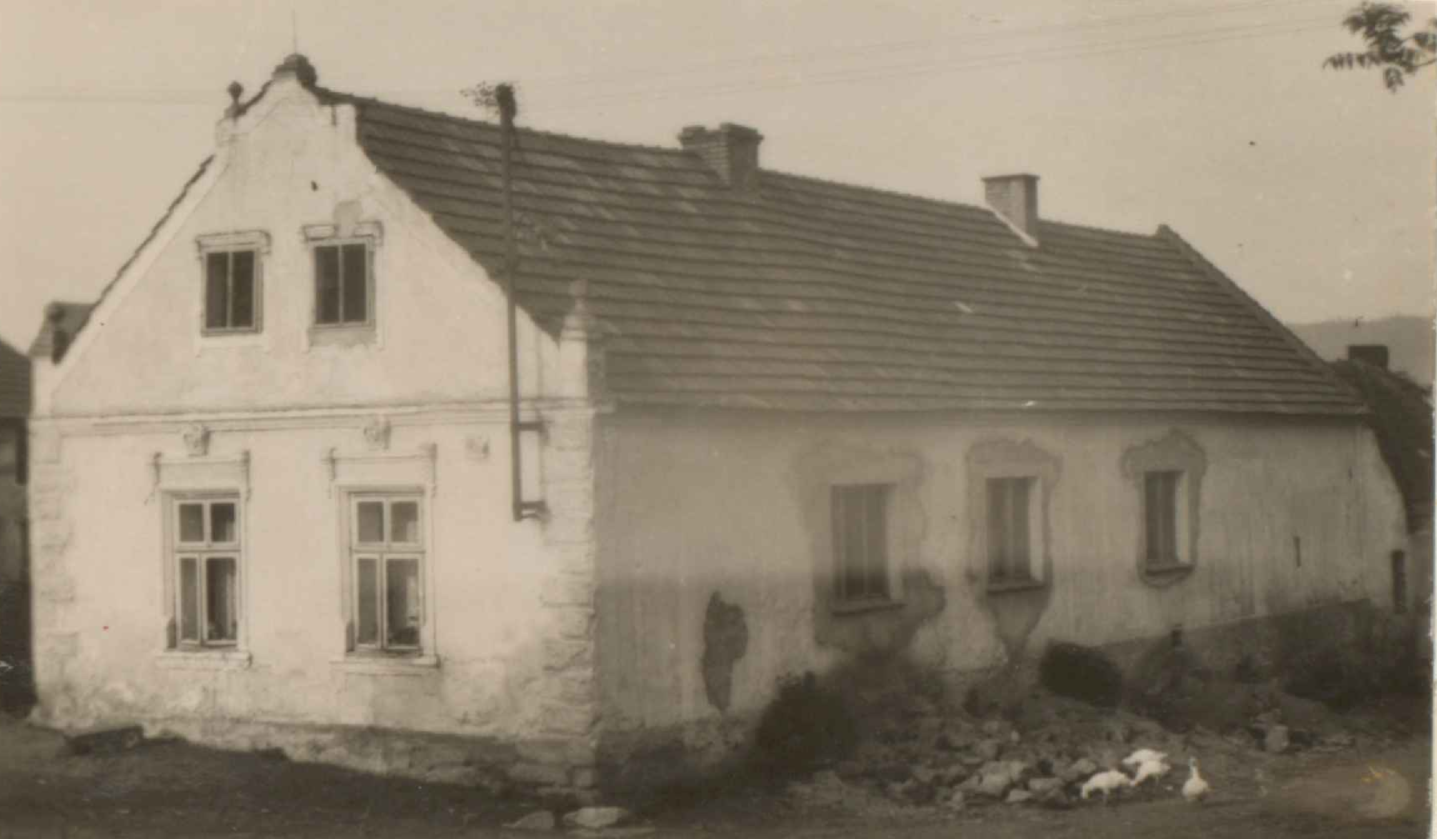
\includegraphics[width=\textwidth, height=\textheight, keepaspectratio]{158-a-statek_v_potvorove}
\caption{Statek v Potvorově }
\label{fig:158-a-statek_v_potvorove}
\end{figure}

\begin{figure}
\centering
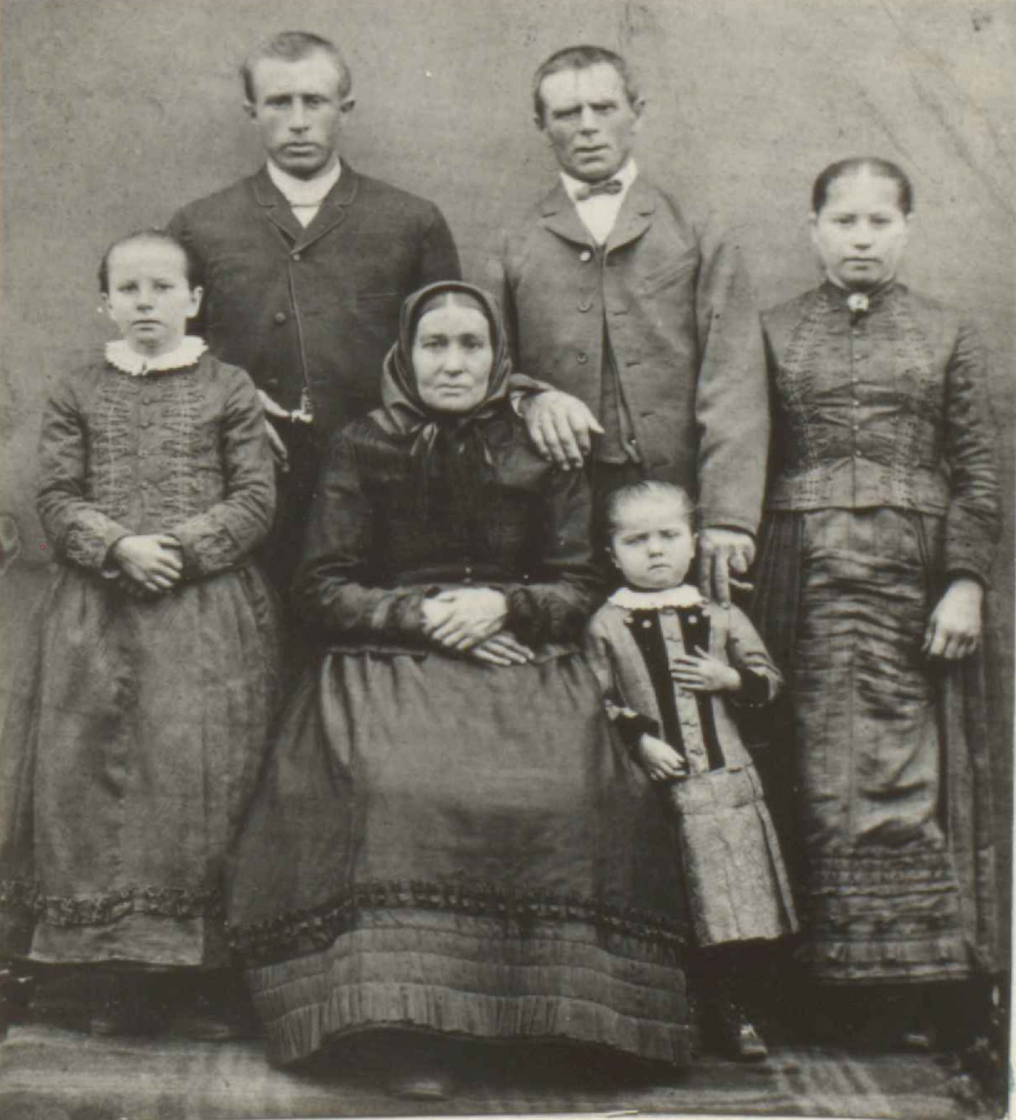
\includegraphics[width=\textwidth, height=\textheight, keepaspectratio]{158-b-marie_prusikova_kozova}
\caption{Marie Prusíková, provdaná Kozová v Potvorově (1845 – 1893)}
\label{fig:158-b-marie_prusikova_kozova}
\end{figure}

% str 138 @ 159
\section{Odnož Chrašťovice - větve Sedlec}

Potomci Vojtěcha Prusíka, rodáka ze Sedlce, usazeného v Chrašťovicich.

1810 - 1882

Vesnice Chrašťovice leží mezi Žíhlí a Mladoticemi v dnešním okrese Plzeň-Sever. V roce 1250 patřily kláš­teru plasskému. V průběhu dějin byla tato obec v ma­jetku mnoha pánů, ale nakonec zůstaly Chrašťovice trvale při hradě Rabštejně. V roce 1654 bylo zde 12 statků. Po třicetileté válce byl jejich majitelem pan Jáchym Libštejnský z Kolovrat na Rabštejně. V této obci, kte­rá dnes má asi 140 obyvatel, usadil se Vojtěch Prusík ze Sedlce.

Vojtěch Prusík narodil se 30. 3. 1810 v Sedlci č. 4. Když bylo doma rozhodnuto otcem Václavem, že rodný grunt převezme jeho nejmladší bratr František, hledala se usedlost a místo pro Vojtěcha. Našla se v Chrašťovicích v čísle 18. Zde se odedávna říkalo "u Šliků". Když 23. 7. 1839 získal Vojtěch Prusík po Bernardu Šlikovi tuto usedlost, byl již několik let ženat. Oženil se 26. 11. 1832 s Barborou Kozovou z Potvorova. Ta se tam narodila 1812, manželé bydleli spolu zpočátku v Potvorově. Tam se jim také narodil první syn Vojtěch i druhý Václav. Teprve Jan a Marie narodili se v Chrašťovicích. Je tedy jméno Prusík v Chrašťovicích od roku 1839 a poslední člen této rodové větve a odnože odešel z Chrašťovic v roce 1960. Byla to dcera Františka Prusíka Marie, provdaná Pastorová, která dnes žije v rodišti svého manže­la v Kněževsi u Rakovníka. V Chrašťovicích žije dnes opět jiný Prusík, ale ten již patří k rodové větvi zva­né Stražište.

Vojtěch Prusík byl velmi dobrým hospodářem, zvláště ko­ně byli jeho oblibou. Ovšem ne jen se strany chovatelské, ale také obchodní. Tuto jeho obchodní zálibu, která značně vynášela, ale někdy až ničila, zdědili i jeho potomci. Vojtěch Prusík měl tři syny a dceru kromě těch dětí, které zemřely v mládí. Jeho žena Barbora ho předešla do hrobu, zemřela 18. 12. 1876, v Chrašťovicích. Vojtěch zemřel 27. 1. 1882.

Prvním jeho synem byl Vojtěch, narozený roku 1835 v Potvorově a měl dostati hospodářství. Zemřel však již mladý, svobodný 9. 4. 1856 v Chraštovicích. Příčinou smrti byla hnisavá angína. Druhým synem byl Václav. Narodil se 6. 8. 1838 a ten pak byl určen jako dědic gruntu. Za manželku měl Marii Kočovou nar. 28. 6. 1837, v Bílově. Ta se pak dožila úctyhodného věku 90 let a zemřela 9. 12. 1927 v Chrašťovicích. Václav Prusík velmi zvelebil used­lost "u Šliků". K tomu mu zvláště také dopomohly úspě­chy v obchodě s koňmi. V tom směru byl veliký odborník a jezdil až do Uher jako později jeho syn Václav. Václav Prusík měl pět dětí. Jeho nejstarší dítě narodilo se 18. 10. 1862 v Bílově. Byl to ještě nemanželský syn Václav,
% str 139 @ 160
ale otec mu dal po svatbě s jeho matkou. Marií, roz. Kočovou, své jméno. Zdědil pak grunt, ale zemřel po­měrně brzy 9. 10. 1899 v Chrašťovicích. Druhý byl syn František, nar. 2. 4. 1870, který zemřel v Chrašťovicích 11. 1. 1934. Třetím dítětem byla dcera Barbora, nar. 5. 11. 1871 v Chrašťovících, provdaná Šmídlová v Mladoticích. Tam zemřela poměrně mladá 12. 9. 1923. Čtvrtým dítětem byl Josef Prusík. Narodil se 14. 3. 1876, vyu­čil se řeznictví a ve svých osmnácti letech odjel do Spojených států. Po těžších začátcích, jak bylo větši­nou souzeno českým emigrantům, usadil se v Chicagu. Tam se stal komisionářem na velkých jatkách, zbohatl, ale nikdy se neoženil. Byl váženým členem mnoha kra­janských spolků. Za ním přijel v prvním desetiletí to­hoto století Václav Prusík, také rodák z Chrašťovic. Josef Prusík zemřel v Chicagu v březnu 1948. K jeho úmrtí bylo napsáno mnoho oslavných nekrologů v tamních krajanských listech. Posledním dítětem Václava Prusíka v Chrašťovicích byl syn Jan. Narodil se v usedlosti "u Šliků" č. 18 dne 26. 5. 1879. Vystudoval obchodní školu a stal se úředníkem pojišťovny v Praze. Nikdy se neoženil. Dlouho bydlel u své neteře Věnceslavy Řehákové v Praze na Vinohradech, kde také zemřel 5. 2. 1954. Na své přání byl pohřben na hřbitově ve Stražišti, jako před tím již jeho otec a děd. Václav Prusík z Chrašťovic zemřel 1. 2. 1884 v Chrašťovicích. Bylo mu teprve 46 let, příčinou smrti byl zápal plic.

Nyní si povíme něco o třech dětech Václava Prusíka z Chrašťovic, které zanechaly potomky. P0 jeho synech Josefovi a Janovi nezůstali žádní.

Dědicem gruntu po Václavu Prusíkoví stal se jeho syn se jménem Václav. Narodil se 18. 10. 1862, vzal si za manželku Aloisii Scherbaumovou, která se narodila v Odlezlech 30. 10. 1870. Václav Prusík, vedle svého hospodářství měl jako jeho otec a děd, největší zálibu v koních a zejména v obchodě s nimi. V tom směru nijak nelenil a zajížděl i do dalekých krajů za tím účelem. Při návratu z jedné takové cesty, na níž promokl, dostal rychlý zápal plic a zemřel 9. 10. 1899. Bylo mu teprve 36 let. Jeho manželka, tak brzo ovdověvší, byla provdá­na podruhé jako Turečková a zemřela v Chrašťovicích 31. 8. 1937. Václav s Aloisií měli tři děti, jen syny. Když tak brzy osiřeli a péče jejich matky nebyla o ně tak vydatná, starala se o ně také babička Marie roz. Kočová a také teta Barbora, provdaná Šmídlová v Mladoticích. Nejstarším synem Václava Prusíka z Chrašťovic byl opět Václav. Narodil se 10. 9. 1890. Vyučil se v koloniálním obchodě v Kralovicích, ale byl to velmi neklidný duch. Jeho touhou bylo podívat se do světa. Již v roce 1905, bylo mu tedy teprve 15 let, odjel za svým strýcem do Chicaga v Americe, u něho však příliš dlouho nepobyl. Jak to v Americe bylo, protloukal se pak v dalších letech všelijak. Někdy se mu dařilo výborně, jindy hůře. V té době vydával se v Americe za potomka starého šlechtického rodu Šliků, jak se u nich na statku říkalo. Za tento podvůdek byl i potrestán.

% str 139+1 @ 161
\begin{figure}
\centering
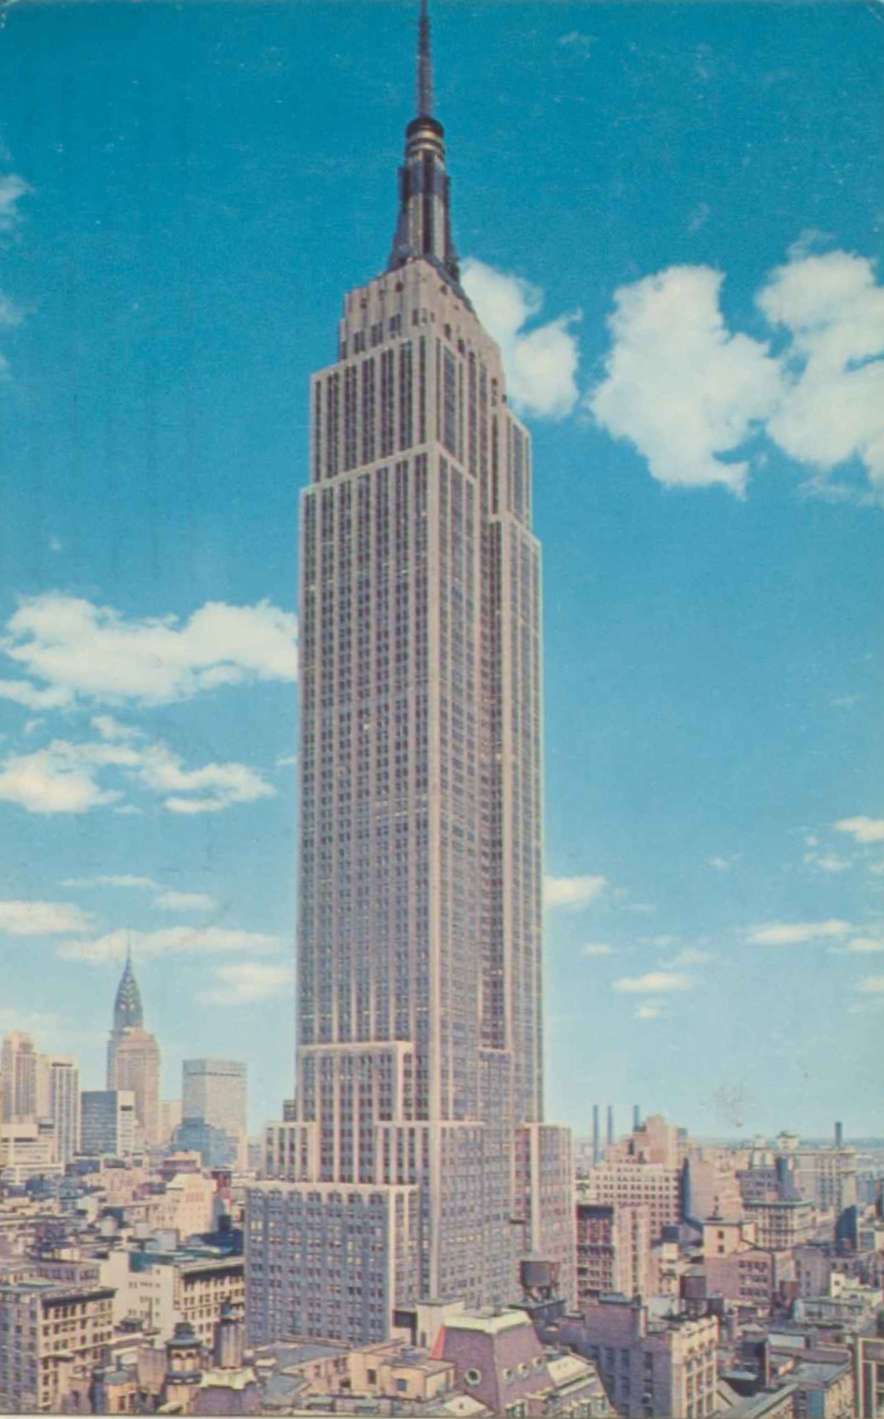
\includegraphics[width=\textwidth, height=\textheight, keepaspectratio]{161-a-nejvyssi_budova_sveta}
\caption{V New Yorku žije Ervín Prusík, člen hodyňské odnože větve Výrov; nejvyšší budova světa v New Yorku}
\label{fig:161-a-nejvyssi_budova_sveta}
\end{figure}

\begin{figure}
\centering
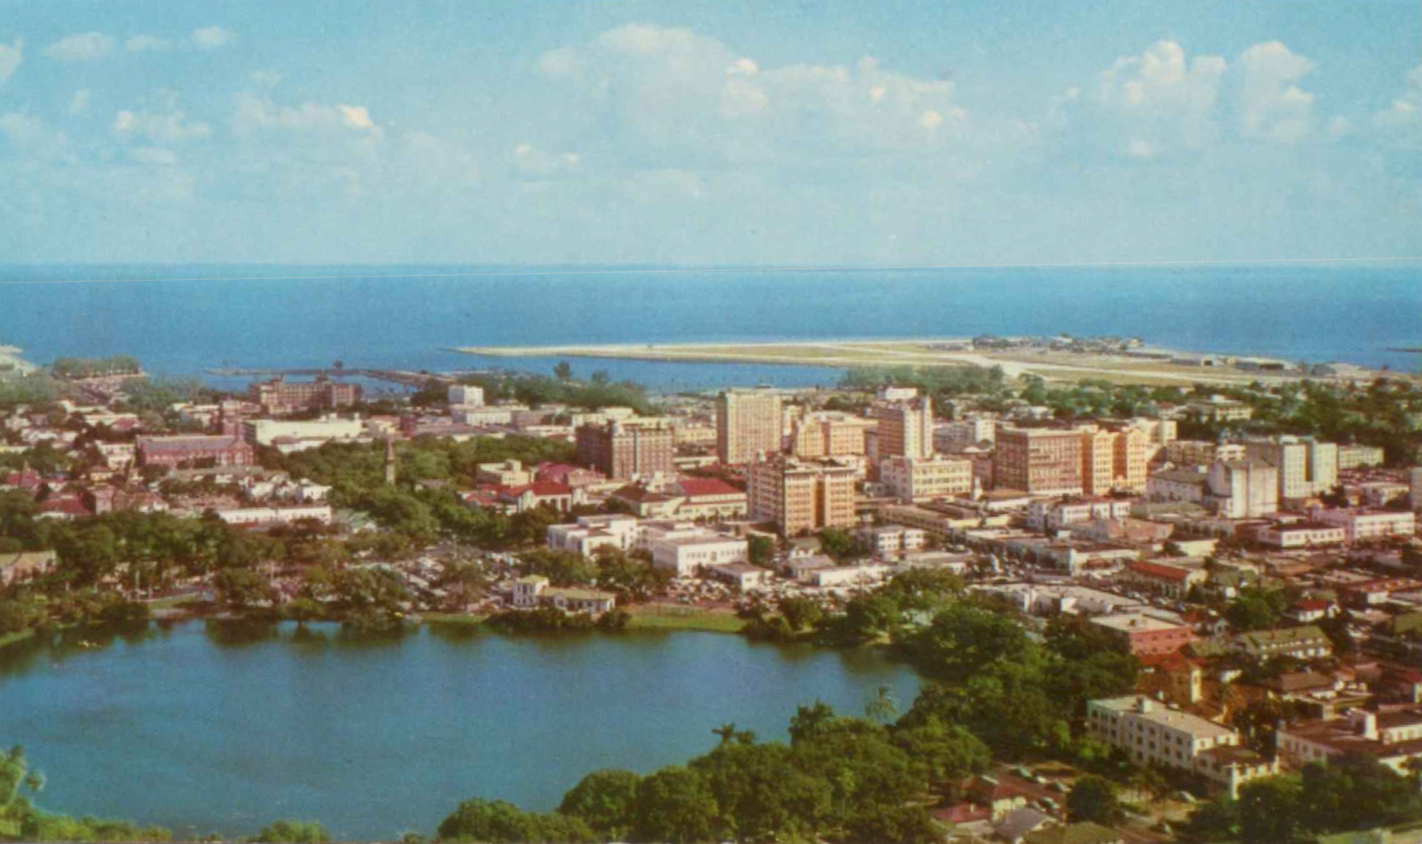
\includegraphics[width=\textwidth, height=\textheight, keepaspectratio]{161-b-st_petersburg}
\caption{Pohled na město St. Petersburg na Floridě v USA. Zde žije Václav Prusík z Chrašťovic}
\label{fig:161-b-st_petersburg}
\end{figure}


% str 140 @ 162
V průběhu mnoha let, které pak Václav Prusík pro­žíval v USA, stal se námořníkem, hercem, obchodníkem a ke konci života se usadil na Floridě, kde bydlí v městě St. Petersburg 5060, 46 th Street. Za manželku má Terezii Guimovou nar. v městě Aurora v americkém státě Nebraska, 7. 12. 1900. Tento Václav Prusík je je­diný z celého našeho rodu, který si pozměnil své jméno na Prusek. Místo Václav dává si raděj i říkati a psáti James. Podle jeho výroků z posledních let lituje tohoto svého činu, neboť žádný Prusík žijící v cizině ani v USA, a není jich málo, něco podobného se svým jménem neprovedli. Václav Prusík má jediného syna Daniela, tedy již Pruseka, který se narodil 23. 8. 1928 v Chicagu. Jak jeho otec, tak i on se však dnes hlásí hrdě k jménu Prusík, ačkoliv toto jméno mají nepatrně pozměněné. Daniel Prusek je obchodním zástupcem velké americké stavební firmy a bydlí v obci Millington ve státě Illinois, nepříliš daleko od Chicaga.  Jeho manželkou je Phyllis Drury narozená 7. 12. 1927 v USA. Mají spolu dvě děti. Dcerka Anna je narozená 14. 7. 1959 a syn James (Jakub) je narozen 4. 4. 1965. Václav Prusík (Prusek) žijící dnes na odpo­činku v půvabném městě na břehu Karibského moře je podruhé ženat. Nynější jeho žena Terezie je původem Němka. První jeho žena byla velmi bohatá. Jmenovala se Ruth a narodila se jako Taylorová v roce 1893 ve Philadelfii a zemřela v říjnu 1927 v Pittsburgu v USA. Václav Prusek, dožívající dnes tak daleko od domova, rád na něj vzpomíná, přestože nikdy od svého odjezdu z vlasti v roce 1905 se sem nikdy nepodíval.

Druhým synem Václava Prusíka, který tak brzy zemřel v Chrašťovicích, byl Josef. Narodil se 11. 2. 1893. O něho, jako sirotka po otci starala se dlouho tetička Barbora Šmídlová v Mladoticích. Josef Prusík vyučil se řeznictví, dobře rozuměl obchodu s dobytkem a také hotelnictví. Určitý čas byl v Praze, pak se zase vrá­til do Kralovic blízko svého rodiště a tam se oženil v roce 1927 s Marií Výškovou, která se narodila 13. 12. 1891 v Nadrybech. Když si ji Josef bral, byla vdovou po majiteli pěkného hostince, Jánském v Kralovicích. Josef Prusík se svou ženou neobyčejné pak zvelebili svůj pod­nik, který se z hostince stal opravdovým hotelem, v Kralovicích nejlepším toho druhu. I když dnes již dávno není Josef jeho majetníkem, přece jen hotel nese stále jeho jméno. Marie Prusíková roz. Výšková zemřela 3. 10. 1965, vdovec Josef Prusík žije nyní na odpočinku ve svém domě v Kralovicích č. 51. Patří v Kralovicích k váženým a velmi oblíbeným občanům. Josef Prusík s Marií měli tři dcery a jednoho syna, když ona před tím již z prvního manželství měla dceru.

Nejstarším dítětem Josefa Prusíka z Kralovic je dcera Alena. Narodila se 23. 8. 1928, provdala se za inž. Sta­nislava Klukovského, dnes úředníka Státní banky. Alena Klukovská je také úřednicí v této bance. Bydlí v Praze 7, Schnirchova č. 28. Mají dcerku Marcelu nar. 2. 4. 1955.

% str 141 @ 163
Druhou dcerou Josefa Prusíka je Jaroslava. Narodila se 19. 3. 1930 a provdala se za Zbyňka Rudu, který je pracovníkem Státních statků. Mají dcerku Janu Rudovou nar. 24. 7. 1954. Ze čtyř dětí Josefových žije dnes ona jediná s tatínkem, vdovcem, v Kralovicích 51. Po těchto dvou dcerách narodil se Josefu a Marii Prusíkovým syn Václav. Bylo to 28. 1. 1932. Vyučil se u Beránků v Praze a dnes pracuje jako kontrolor Restaurací a jídelen v Plzni pro okres Plzeň-sever. Jeho manželkou je Marta Pivoňková nar. 14. 9. 1936 v Nahošovicích u Domažlic. Václav Prusík se svou ženou Martou bydlí v Nýřanech 312 u Plzně. Mají dva syny. Michal je narozen 20. 2. 1960 a Vladimír 11. 2. 1962. - Posledním dítětem bývalého hoteliéra Josefa Prusíka z Kralovic je dcera Dana. Narodila se 18. 7. 1939. Je dnes provdána za pracovníka Stát­ních statků inž. Jana Kutého, rodáka z Moravy. Tam také nyní žijí v Pěnčíně č. 68 v okrese Prostějov. Mají dvě děti. Danu nar. 8. 7. 1962 a Jana Kutého nar. 7. 1. 1964.

Třetím synem Václava Prusíka z Chrašťovic byl František. Narodil se 8. 3. 1897. Vyučil se řeznictví, nějaký čas měl také svůj hostinec v Mladoticích, ale pak se natrvalo usadil ve Výrově-Hadačce č. 47. Jeho manželka Anna Soprová pocházela z Hodovíze, kde se narodila 5. 3. 1897. Zemřela ve Výrově 22. 7. 1956. Její muž František Prusík zemřel v nemocnici v Kralovicích 27. 6. 1964. František Prusík s Annou měli čtyři děti, dva syny a dvě dcery. Nejstarší je Božena nar. 2. 2. 1924. Vzala si úředníka Karla Štégla a bydlí v Kralovicích č. 83. Mají dvě děti, Miloše nar. 19. 1. 1949 a Evu nar. 6. 12. 1952. Další je František Prusík, nar. 1. 11. 1928. Otec ho dal také vyučit řeznictví a určitou dobu byl zaměstnán na pražských jatkách. Dnes je šoférem Stavebního podniku v Krnově ve Slezsku, náměstí Osvobození č. 8, kde bydlí. Jeho manželkou je Moravanka Soňa Pochylová. Narodila se 6. 9. 1931 v Koryčanech u Kyjova. František a Soňa ma­jí spolu dvě dcery. Soňa Prusíková se narodila 1. 9. 1952 a druhá Iva je narozená 9. 8. 1954. Obě tato děvčata hra­jí pěkně na trubky a jiné dechové nástroje a procesto­valy již s orchestry pěkný kus Evropy.

Druhou dcerou Františka Prusíka z Výrova, je Věra. Narodila se 13. 1. 1931 a provdala se za rolníka Jarosla­va Ždánského. Žijí spolu v rodišti manželové Sukoradech 65 u Mladé Boleslavě, kde pracují v JZD. Mají čtyři děti. Jaroslav Ždánský je narozen 30. 4. 1950, Věra 6. 6. 1952, Miloš 25. 1. 1958 a Jiří 3. 12. 1962.

Posledním dítětem Františka Prusíka z Hadačky a Jeho ženy Anny je syn Pavel. Narodil se 23. 7. 1943. Bydli v domku svých rodičů ve Výrově-Hadačce. Jeho ženou je Dana roz. Levá 6. 2. 1946 ve Výrově. Pavel Prusík absolvoval země­dělskou meliorační školu a pracuje dnes jako mechánisátor v JZD ve Výrově.

% str 142 @ 164
Druhým synem Václava Prusíka z Chrašťovic, naroze­ného v roce 1838, byl František Prusík. Narodil se 2. 4. 1870. Po svém, brzy zemřelém bratru Václavovi převzal hospodářství a pak žil v usedlosti své ženy, kam se přiženil. Vzal si ji v pozdějším věku. Byla to Marie Churavá, narozená 2. 4. 1883 v Chrašťovicích. A zase i tento Prusík, jako snad všichni chrašťovičtí Prusicí, měl velkou zálibu v koních. Jezdil je nakupovat na Slovensko, do Maďarska a po celé republice. Měl jedinou dceru Marii, která se narodila 29. 12. 1920. Otci tedy již bylo padesát let. Marie provdala se za Josefa Pastora, který za okupace působil jako finanční úředník na protektorátní hranici, která nedaleko Chrašťovic probíhala. František Prusík, poslední hospodář toho jména odnože chrašťovické, zemřel 10. 1. 1934 v Chrašťovicích. Vdova po něm, Marie odešla na věčnost 26. 5. 1950.

Jejich dcera Marie, provdaná Pastorová hospodařila pak doma, ale v roce 1960 odstěhovala se na naléhání své­ho manžela do jeho rodiště Kněževse u Rakovníka, kde je bohatý chmelařský kraj. Tam bydlí v čísle 332. Její syn, Josef Pastor narodil se 30. 5. 1945.

Dalším dítětem Václava Prusíka z Chrašťovic, po němž zůstali potomci, byla dcera Barbora. Narodila se 5. 11. 1871 a provdala se za majitele hostince a hospodářství Josefa Šmídla v Mladoticích. Starala se obětavě o své synovce, když její bratr Václav tak brzy zemřel. Ale ani ona dlouho nežila. Zkosila ji chřipka 12. 9. 1923 v Mladoticích. Barbora Šmídlová, roz. Prusíková měla tři děti. Nejstarší je syn Oldřich Šmídl, narodil se 14. 3. 1900. Zůstal doma na hostinci a až dodnes je soukro­mým hospodářem. Neustoupil ani tomu největšímu nátlaku doby. Bydlí v Mladoticích č. 47. Má čtyři děti. Jeho syn Jiří Šmídl se narodil 25. 12. 1928. Bydlí v Lubenci č. 71, kde pracuje v podniku TOS. Má dvě dcerky. Jarmilu Šmídlovou nar. 2. 3. 1959 a Ivu nar. 10. 6. 1963. Druhý syn Oldřich Šmídl, nar. 30. 3. 1930 je svobodný. Je elektrotechnikem. Dcera Jarmila rozvedená Holotová, narodila se 17. 8. 1933 a má dcerku Marcelu, nar. 23. 9. 1961. Její sestra Eliška Šmídlová nar. 28. 5. 1947 bydlí s ní v Karlových Varech, respektive Nové Roli č. 212.
Druhým dítětem Barbory Šmídlové, roz. Prusíkové byla dcera Božena. Narodila se 21. 5. 1901 v Mladoticích a provdala se za zaměstnance justiční služby v Praze, rodáka ze Stvolného u Rabštejna, Heidenreicha. Bydlí v pěkné vilce v Praze - Kunraticích, Mašátova 441. Heidenreichovi mají jedinou dceru Dagmar nar. 10. 8. 1927. Je lékařkou. Dosti dlouho působila v nemocnici v Duchcově a nyní jako odborná lékařka vnitřních nemocí v Praze 7. Je provdaná Kleinová a její muž je také lékařem. Bydlí v Praze - Vyšehradě, Vratislavova 30. Dr. Dagmar Kleinová má dvě děti. Dcerku Dagmar nar. 14. 6. 1961 a synka Oto, nar. 19. 3. 1963. Třetí dítě Barbory byla dcera Věnceslava. Narodila se 28. 9. 1905 a jako provdaná Řeháková v Praze byla zabita autem na ulici 1o. 10. 1963. Děti neměla.

% str 143 @ 165
To byly tedy osudy v kostce všech potomků Václava Prusíka z Chrašťovic, jehož otec Vojtěch se narodil roku 1810 v Sedlci.
Třetím synem Vojtěcha Prusíka, usazeného v roce 1839 v Chrašťovicích, byl syn Jan. Narodil se 18. 1. 1841, ale rodný statek mu nebyl určen. Proto hledal, kde by se uchytil. A tu naskytla se koupě v Újezdě u Manětína. Tato vesnice má sotva 70 obyvatel, bývala v majetku různých vrchností, také Šliků z Rabštejna, Švamberků, kláštera plasského, ale nakonec patřil Újezd panství hraběte Lažanského v Manětíně. Jan Prusík, rodák z Chrašťovic, oženil se s Marií Šmídlovou, narozenou 12. 7. 1843 v Rybnici. Bydleli spolu krátkou dobu ve Stražišti a 3. 8. 1871 zakoupili grunt č. 10 v Újezdě u Manětína. Za usedlost dali dosavadním majitelům manželům Tobiáškovým 6.250.- zlatých. Osud celé této rodiny byl značně pohnutý. Koňařská vášeň chrašťovických Prusíků se zde nevyplatila. Jan Prusík nebyl zvlášť dobrým hospodářem a jeho hlavní vášní byli koně a obchod s nimi. Nepodařenými obchody zadlužil pomalu své hospodářství tak, že brzy po jeho smrti museli je jeho potomci upustit. Dnes v Újezdě nenajdete již ani stopy po stavení, kde Jan Prusík rodák z Chrašťovic se svou rodinou žil. Jan zemřel 22. 2. 1883 a jeho žena 1. 9. 1910.

Jan Prusík měl šest dětí. Jeho dcera Josefa narodila se 1. 6. 1876 v Újezdě. Vdala se za Jana Pešičku ze Hvozda. Josefa Pešičková roz. Prusíková měla pět dětí. Nejstarší byl Václav, nar. 20. 7. 1897. Hned na začátku první světové války odešel na frontu a nejdéle sloužil v Alpách na italské frontě. Když na podzim v roce 1918 skončila válka, utichly zbraně, toužil po tom, aby se dostal co nejrychleji domů. Když nemohl se dostati do přeplněných vagónů, cestoval ještě s několika kamará­dy na střeše železničního vozu. To se mu stalo osudné. Při průjezdu tunelu v Alpách byl zabit jako jeho kama­rádi, kteří volili tento způsob jízdy domů. Druhý byl Stanislav Pešička. Narodil se 3. 4. 1909 v Újezdě u Manětína. Dnes pracuje v lese a bydlí v Lešovicích č. 11 u Nečtin. Až do smrti žila u něho jeho matka, kte­rá tam zemřela 26. 3. 1956. Josefa Pešičková roz. Prusíková měla pak dceru Josefu. Narodila se 28. 2. 1912. Je pro­vdaná Hlávková a bydlí v Kopistech u Mostu, ulice Karla Havlíčka Borovského č. 406. První její dcera, nemanžel­ská Anna, narodila se 9. 2. 1930. Je provdaná Šimicová a bydlí také v Kopistech. Má čtyři děti. Jsou to všechny dcery. Jitka, nar. 5. 6. 1951, Jaruška 12. 8. 1959, Eva 24. 12. 1960 a Ivana Šimicová nar. 8. 7. 1963. Z manželství s dělníkem Hlávkou má Josefa roz. Pešičková pět dětí. Její syn Josef Hlávka nar. 19. 7. 1944 je již ženatý a má synka Romana, nar. 6. 12. 1967. Dále jsou Václav Hlávka nar. 12. 8. 1946, Marie nar. 19. 2. 1949, Jaroslav nar. 7. 11. 1950 a Jitka Hlávková nar. 17. 3. 1952. Všichni žijí v Kopistech u Mostu. Další dítě Josefy Pešičkové, roz. Prusíkové je syn Jan Pešička. Narodil se 9. 8. 1913, je svobodný a pracuje v dolech a bydlí v Kopistech, Marxova 357.

% str 144 @ 166
Posledním dítětem Josefy Pešičkové byla dcera Marie. Narodila se 6. 12. 1919. První její dcera byla nemanželská a dostala jméno Marie. Narodila se 8. 1. 1936 a poprvé byla provdána Charitunová, nyní Černá. Bydlí v Břežánkách u Teplic, Hornická 98. Má synka Jana Charituna nar. 6. 7. 1954. Marie Pešičková se pak provda­la za Jihoslovana Galjaniče, žila s ním na Teplicku a později odstěhovali se do Křečova u Manětína. Bylo jí pouze 47 let když tam zemřela na rakovinu 30. 3. 1966. Z jejího manželství narodili se dva synové.  Václav Galjanič 13. 9. 1946, který dnes je zaměstnán a bydlí v Hodoníně, Havlíčkova 1. Druhý Pavel Galjanič žije s otcem-vdovcem. Narodil se 6. 6. 1951.

Jan Prusík se svou ženou Marií, usazený v Újezdě u Manětína, měl dva syny a těšil se, že jeden z nich stane se dědicem gruntu. Tyto plány se však úplně zhatily. Jednak nastal úplný úpadek tohoto statku a ta­ké oba synové, svobodní, brzy zemřeli. Václav na­rodil se 9. 9. 1870 ve Stražišti. Byl na vojně, tam onemocněl a brzy potom zemřel doma v Újezdě, svobod­ný, 4. 1. 1896. Jeho bratr František Prusík, nar. 19. 7. 1873 v Újezdě odešel také na vojnu a i jemu stala se osudnou. Vážně tam onemocněl, poslali ho z vojny domů, ale tam jako 22letý zemřel 1. 4. 1895.

Další dcerou Jana Prusíka byla Terezie. Narodila se 25. 9. 1882. Svého otce ani nepoznala a její život byl velmi těžký. Vyučila se švadlenou a často ani nemíva­la dost práce. Teprve když se vdala za Františka Přibyla, dělníka na Mostecku, začalo se jí dařit o něco lépe. Žila v Kopistech. Jediným jejím dítětem byla dcera Zdeňka. Narodila se 18. 5. 1916 a je provdaná Háková v Mostě, ul. Gottwaldova č. 2817. Má dvě děti. Její syn Václav Hák nar. 1. 7. 1943 je učitelem, dcera Jitka Háková nar. 18. 10. 1944 má nemanželskou dcerku Šárku, nar. 27. 6. 1967. Terezie Přibylová, roz. Prusíková zemře­la v Kopistech u své dcery 9. 12. 1959.

Další dcerou Jana Prusíka byla Anna. Narodila se 6. 8. 1862 a provdala se za Ondřeje Pešíka. Zpočátku snažili se oba manželé zachránit statek v Újezdě lepším hospodařením, ale to se již nepodařilo. Odstěhovali se do Plzně, kde manžel Anny Pešíkové, roz. Prusíkové byl zaměstnancem drah. Měli tři dcery. Nejstarší je Anna Pešíková, která se neprovdala. Narodila se 16. 7. 1894 a bydlí v Plzni, Fučíkova 34. Ta má snad nejlepší přehled o osudech celé rodiny Jana Prusíka. Její sestra Krista provdaná Burgetová, narodila se 8. 9. 1896 a zemřela v Plzni 4. 12. 1962. Její manžel byl úředníkem drah. Třetí dcerou Anny Pešíkové roz. Prusíkové, je Anastazie, provdaná Niklfalterová. Je narozena 14. 4. 1903 a bydlí se sestrou Annou v Plzni. Žádná z nich neměla děti.

% str 145 @ 167
Špatný osud měla také dcera Jana Prusíka z Újezda, Albína. Narodila se 20. 12. 1879 v Újezdě a provdala se za horníka Václava Havlíka do Kopist na Mostecku.. Měla dvě dcery, Marii nar. 1907, která byla provdaná Novotná a zemřela bezdětná v roce 1928 v Kopistech. Druhá dcera Emilie Havlíková narodila se v roce 1912 a zemřela, když jí bylo 15 let v roce 1927. Ani Albína Havlíková roz. Prusíková nežila dlouho. Zemře­la ve svých 44 letech na souchotiny v roce 1923 v Kopistech.

Po Janu Prusíkovi, rodáku z Chrašťovic nezůstal te­dy žádný mužský potomek, po němž by žili zase Prusíci a ani osud jeho dcer nebyl vždy nejlepší. Bývá to tak někdy v životě.

Posledním dítětem Vojtěcha Prusíka, rodáka ze Sedlice a usazeného v Chrašťovicích, byla dcera Marie. Narodi­la se 1. 8. 1845. Její matka byla rozená Kozová z Potvo­rova a tak se dohodlo, že dcera se zase provdá do je­jího rodu. Poněvadž jejím sňatkem vznikla by příbuzenskost třetího stupně, bylo třeba zažádati o zvláštní povole­ní ke sňatku. Marie Prusíková provdala se pak 12. 11. 1861 za Václava Kozu v Potvorové č. 47, kde se říkalo odedávna "u Kordů". Václav Koza měl v Potvorové hospodářství. Narodil se 1. 8. 1839.  Marie Prusíková byla, pokud máme v historii zaznamenáno, druhým pokrevním členem našeho rodu, který se dostal do Potvorova. Před ní byla v první polovině XVIII. století dcera Martina Prusíka ze Sedlce, Eva, která se tam provdala k Hrdíkům.

Potvorov je prastará obec a píše se o ní již ve XII. století, kdy tam byl vladykou Humpolt. Na konci XII. století byl v Potvorové vladycký dvůr otočený příkopem a náspem jako tvrz. V nádvoří stál románský kostel, který rovněž byl obehnán příkopem, jejž místy lze dosud pozorovati. Ze dvora vedl krytý pavlán na kostelní kruchtu. V čase nebezpečí se sem uchylovali obyvatelé vesnice. Tento prastarý románský kostel sv. Mikuláše v Potvorově, nejstarší v celých západních Čechách, je pro nás památný tím, že zde byli křtěni, ženili a vdávaly se a byli pohřbíváni, všichni naši dávní předci ze Sedlce.

V Polovině XVII. století nikde není jmenováno ještě jméno Koza v této obci. Přišel patrné tento rod mnohem později do Potvorova.

Marie Kozová se svým mužem Václavem měla sedm dětí, které dospěly. Byli to synové Josef, Václav, František a Jan a dcery Barbora, Marie a Františka. Marie Kozová rozená Prusíková byla, jak pamětníci dokazují, výbornou hospodyní a dovedla se dobře otáčet nejen ve svém statku, ale i všude jinde. Dlouhého věku se však nedožila, zemřela na souchotiny 22. 6. 1893 v Potvorově. Její muž Václav ji přežil o 22 let. Zemřel 18. 5. 1915.

% str 146 @ 168
Nejstarším dítětem Marie Kozové, roz. Prusíkové byl syn Josef. Narodil se 20. 1. 1863 a v Potvorově hospodařil. Měl šest dětí. První byl František Koza. Narodil se 31. 10. 1890 a zemřel 24. 9. 1922. Pomáhal doma v hospodářství a jeho neštěstím bylo, že byl hluchoněmý od narození. Stejně tak bylo s jeho bratrem Mikulášem. Ten se narodil 22. 2. 1894 a pro stejný neduh zůstal také doma u rodičů a zemřel ve svých třiceti letech 12. 6. 1924. Asi se zde projevil neblahý vliv příbuzenského sňatku jeho babičky. Dalším dítětem byla Marie. Narodila se 21. 8. 1897, na různých místech mimo domov sloužila jako hospodyně, pak byla provdána Nováková a dnes jako vdova žije v Mostě, ul. Maxima Gorkého 986/6. Nemá dětí, má však výborný přehled o celé své rodině Kozů jako málokdo. Čtvrtým dítětem Josefa Kozy, který zemřel 21. 9. 1926, byl syn Bohuslav Koza. Narodil se 28. 5. 1900 v Pot­vorově, zůstal svobodný a také pomáhal jako předtím jeho bratři František a Mikuláš, všude a zvláště na statku svých rodičů. Zemřel také mladý, 27. 5. 1931. Pátá je Hedvika, nar. 17. 10. 1902. Je provdaná za vdovce Koubu, s nímž však neměla dětí a bydlí v Potvorové č. 73.

Posledním byl Josef Koza. Narodil se 4. 1. 1907 a měl dostati doma hospodářství. Také skutečně pak na rodném svém gruntě hospodařil, ale ani on dlouhého věku ne­dosáhl a zemřel na souchotiny 17. 1. 1942 v Potvorově. Měl dvě děti. Jeho syn Josef nar. 6. 2. 1933 pracuje v průmyslu v Děčíně a tam také bydlí ve Foersterově uli­ci č. 863-14. Je podruhé ženatý, a z těchto dvou manžel­ství má vždy po jednom chlapci. Josef Koza nar. 20. 11. 1955 a Zdeněk Koza nar. 8. 12. 1957. Druhým dítětem Josefa Kozy v Potvorově byla dcera Marie. Narodila se 28. 4. 1935, je provdaná Jandová a je učitelkou. Má dvě dě­ti, Jiřího Jandu nar. 24. 6. 1961 a Janu nar. 1. 4. 1964. Bydlí v Plzni, Mánesova 89.

Druhým dítětem Marie Kozové. roz. Prusíkové byl syn Václav. Narodil se 17. 10. 1864 a přiženil se v obci do čísla 16, kde se již po třicetileté válce říkalo "u Vicendů". Václav Koza měl pěkné hospodářství a býval také starostou. Měl tři děti. Jeho dcera Marie nar. 8. 4. 1897 byla provdána za dílovedoucího drah Woldána. Měli svůj domek v Rokycanech, kde zemřela 12. 5. 1949. Dětí neměla. Druhé dítě Václava Kozy je syn Václav, narozený 28. 8. 1899 a převzal po otci hospodářství, které je dnes začleněno do JZD. Také tento Václav Koza byl dlouho starostou obce a zvláště za okupace se v této funkci neobyčejné osvědčil. Má tři děti. Jeho dcera Věra, nar. 4. 11. 1924 je provdaná Fryčková. Bydlí v Dobřanech na nádraží, kde je její manžel náčelníkem stanice. Ona pracuje jako zdravotní sestra v psychiatrické léčebně v Dobřanech. Má dvě dcery. Jaroslavu Fryčkovou nar. 10. 7. 1951 a Věru nar. 25. 8. 1962. Pak je syn Václav nar. 20. 2. 1930. Oženil se a převzal jméno po své manželce, Tichý. Bydlí v Plzni-Doubravce, Smrková 20. Má synka

% str 147 @ 169
Pavla Tichého nar. 13. 10. 1964. Druhý syn Václava Kozy je Jaromír, nar. 17. 5. 1932. Bydlí v Kralovicích tř. Rudé armády 29. Je zaměstnán u ČSAD. Má dvě děti, Marcelu Kozovou nar. 4. 5. 1959 a Milana Kozu nar. 9. 5. 1961. Třetím dítětem Václava Kozy, který se přiženil k Vicendům, byl syn František. Narodil se 31. 3. 1901 a po celý život byl zaměstnán u dráhy. Zvláště dlouho působil na Ústecku, odkud pochází jeho žena. Manželství jejich je bezdětné. František Koza žije nyní na odpočinku v Praze 6-Dolní Liboci, Litovická 9.

Václav Koza z Potvorova, otec Marie, Václava a Františka zemřel poměrně opuštěn doma 13.  6. 1941. Jeho syn Václav zemřel 12. 6. 1968.

Dalším synem Marie Kozové roz. Prusíkové byl syn František. Narodil se 14. 8. 1867. Měl v Potvorově hos­podářství, řeznictví a hostinec. Byl dvakrát ženatý, z prvního manželství měl pět dětí a z druhého dvě. František Koza, který byl v obci velmi oblíben, zemřel v Potvorově 2. 8. 1946.

Nejstarším dítětem Františka Kozy byl syn Bedřich. Narodil se 4. 2. 1894, vyučil se řeznictví a zůstal svobodný. Zemřel v Potvorově 8. 10. 1957. Druhý, Josef Koza nar. 9. 3. 1895 byl vyučen číšníkem, po vypuknutí první světové války byl hned povolán a padl 30. 12. 1915 na ruské frontě u Stryje v Haliči. František Koza měl pak dceru Marii, nar. 4. 9. 1899. Vzala si za manžela opět Kozu, který ovšem nepatřil do potomků Marie Prusikové. Byl traťmistrem v Příbrami a tam také Marie Kozová zemřela 23. 11. 1951. Měli jediného syna Jana Ko­zu, který se narodil 29. 6. 1930 a je zaměstnán u ČSAD jako dispečer. Je svobodný a bydlí v Příbrami IV, ul. Čsl. armády 154.

Další dítě Františka Kozy z Potvorova byl syn František. Narodil se 31. 5. 1897 a dlouhá leta byl úředníkem u drah, zvláště také dlouho působil na Ústecku jako jeho bratranec František. V pozdějším věku se František Koza oženil, ale děti již neměl. Ke konci života bydlel v Praze 7. Pro svůj nesmlouvavý politický postoj po únoru 1948 odešel ze služby ČSD a působil pak na různých místech, naposled jako úředník v sanatoriu v Dobříši. I on měl přehled o široké rodině Kozů a vždy se hlásil také k našemu rodu Prusíků. Zemřel náhle 4. 1. 1965 v Praze.

Dalším dítětem Františka Kozy z prvního manželství byl syn Vladimír. Narodil se 2. 8. 1902 a hospodařil v Potvorově č. 43. Jeho zdraví však nebylo valné a zemřel 26. 7. 1964. I on byl v obci velmi oblíben. Vladimír Koza měl dvě dcery. Božena nar. 10. 5. 1929 je provdaná Jandová v Kralovicích, Plzeňská 15. Má dvě děti. Vladimíra nar. 12. 12. 1953 a Danu nar. 9. 8. 1958. Druhá dcera Drahuše narodila se 26. 7. 1931. Je provdaná Cepková a bydlí v Potvrově č. 60. Má tři děti. Libuši nar. 26. 12. 1953, Josefa nar. 24. 3. 1955 a Pavla Cepka nar. 23. 10. 1956. Posledním dítětem z prvního manželství Františka Kozy Byla dcera Božena. Narodila se 6. 1. 1905 a také na ní se opět projevily neblahé důsledky někdejšího příbuzenského
% str 148 @ 170
sňatku její babičky. Dali ji sice z domova na zvláštní léčení do Jilemnice, ale Božena Kozová zemřela tam jako jedenáctiletá 28. 12. 1915. Z druhého manželství Františka Kozy narodili se ještě dva synové. Václav Koza narodil se 4. 5. 1911 a dnes působí a bydlí v Kraslicích, Komenského 1513. Má dvě děti, dceru Evu nar. 26. 8. 1938 provdanou Farskou. Je úřednicí a má dva syny Milana nar. 25. 11. 1958 a Jiřího Farského nar. 14. 3. 1960. Syn Václava Kozy Petr, narodil se 13. 2. 1944. Je chemikem a to v podniku Amati.

Druhým synem Františka Kozy z jeho druhého manželství je Blažej. Narodil se 26. 1. 1914 a bydlí v Potvorově 28. Měl svůj hostinec a pracoval také ve výkupu zemědělských výrobků. Má jediného syna Bohuslava Kozu narozeného 17. 3. 1937. Je stavebním technikem a bydlí v Kralovicích-Sídlišti č. 559. Má dvě dcerky, Bohuslavu Ko­zovou nar. 6. 9. 1962 a Jarmilu Kozovou nar. 6. 2. 1967. Také z Potvorova emigrovali členové rodu do USA. Čtvrtým synem Marie Kozové roz. Prusíkové je syn Jan. Narodil se 5. 5. 1875. Vyučil se řeznictví a byl to vel­mi podnikavý člověk. Na začátku XIX.století odjel jako mnoho Čechů do USA a usadil se nakonec ve státě Iowa, městě Iowa City. Tam měl své řeznictví a zúčastnil se i jiného podnikání jako důlní těžby a velmi zbohatl. Oženil se s Američankou, ale zdá se že toto manželství nebylo příliš šťastné. Jezdíval občas do své vlasti a vyjadřoval se, že se ke konci života vrátí do Čech a trvale ve svém domově usadí. Když se k tomu v Americe chystal a připravoval k odjezdu, zemřel náhle 5. 4. 1947. Jan Koza měl dvě děti. Jeho dcera Alice narodila se 14. 2. 1905 a je provdaná za obchodníka McCollistera. Bydlí nyní v lesnatém a jezernatém kraji ve státě Minne­sota v městečku Cross Lake. Alice má tři děti. Nejstarší je syn Robert, nar. 27. 7. 1928 a je lékařem. Pracuje na klinice university v Minneapolis, bydlí v městě Edina  6704, Brittany Road. Dr Robert McCollister má dva synky, Karla nar. 5. 1. 1963 a Bruce nar. 8. 9. 1966. Druhým dítětem Alice roz. Kozové je syn Terry, nar. 3. 5. 1934. Je inženýrem a bydlí v místě Cape Elisabeth blízko města Portlandu u Atlantického oceánu ve státě Maine. Inženýr Terry McCollister má dva syny. Jana nar. 7. 7. 1959 a Jakuba nar. 17. 12.  1961.

Třetí je Zuzana narozená 9. 9. 1938, dnes provdaná Zielinová. Je učitelkou. Děti zatím nemá. Bydlí v men­ší obci Minnetonka č. 5808 Scenic Drive ve státě Minnesota. Jan Koza měl syna Jana, nar. 27. 5. 1907. Bydlí v Iowa City a má syna Jana, nar. 15. 7. 1948. Jsou v Hutchinson Ave 340. První dcerou Marie Kozové roz. Prusíkové byla dcera Barbora. Narodila se 31. 5. 1877. Měla nemanželské dítě, dcerku Marii nar. 29. 12. 1897. Barbora se neprovdala a zemřela v Potvorově jako první ze všech dětí Marie Ko­zové roz. Prusíkové před první světovou válkou 2. 7. 1911. Její dcera Marie byla pak provdaná Vavřičková a odstě­hovala se do rodiště svého muže do Zborov č. 25 u Plánce. Tam měli hospodářství. Marie Vavřičková měla sedm
% str 149 @ 171
dětí. První její dcera Vlasta Vavřičková narodila se v roce 1918 a od narození byla slepá. Zemřela svobodná ve svých dvaceti letech v roce 1938. Druhá byla Marie nar. 25. 3. 1921. Provdala se za děl­níka Škodovky Ibra a bydlí v Plzni, tř. 1. máje 71. Má jediné dítě, syna Václava nar. 9. 7. 1946. Další je dcera Alžběta, která se narodila 3. 11. 1922. Je provdaná Sladká a bydlí v Žíhli č. 201. Má tři syny. Karel Sladký se narodil 16. 11. 1943 a bydlí v Jaroměři, Lidická 1. Druhý Jiří, nar. 26. 11. 1947 a Milan Sladký nar. 12. 12. 1955 bydlí doma s rodiči. Čtvrtou dcerou Marie Vavřičkové roz. Kozové je Františ­ka. Narodila se 3. 12. 1924 ve Zborovech a žije dnes v Plzni, U Radbuzy č. 4. Je provdaná Pohanková a má dvě dcery. Věru nar. 9. 1. 1951 a Miluši nar. 8. 2. 1953. Další je Emilie nar. 19. 12. 1926 provdaná Šebestová. Žije také v Plzni, U trati č. 3. Má jediné děcko, dceru Vladimíru nar. 11. 3. 1956.

Poslední dcerou Marie Vavřičkové je dcera Jaroslava. Narodila se 9. 5. 1929 a provdala se za zemědělce Holého. Oba pracují v JZD ve Zborovech č. 25. Jaroslava Holá má dcerku Danu nar. 29. 7. 1953. Jediným synem Marie Vavřičkové byl Karel. Narodil se 21. 10. 1931 a je zaměstnán v Plzni. Tam bydlí v Křižíko­vých sadech. Má dvě děti, Drahuši nar. 4. 2. 1960 a synka Karla Vavřičku nar. 26. 7. 1961.

Druhou dcerou Marie Kozové roz. Prusíkové z Chrašťovic byla Marie. Narodila se 1. 7. 1881 v Potvorově a provda­la se za A. Rozmaru, menšího zemědělce v Potvorově. Po druhé světové válce bydleli v Žíhli. Marie Rozmarová zemřela 26. 4. 1948. Měla dvě děti. Její syn František Rozmara, nar. 16. 6. 1903 byl zaměstnán u dráhy a zůstal svobodný. Po druhé světové válce žil v Chomutově. Při návštěvě svého rodiště Potvorova, zemřel náhle 2. 10. 1963. Druhý syn byl Josef Rozmara. Narodil se 20. 2. 1910 v Potvorově a po květnu 1945 usadil se v Žíhli, kde byl dosti politicky angažován. Byl také zaměstnán u dráhy. Při honitbě na jaře 1949 byl postřelen a brzy podlehl tomuto zranění. Zemřel v Žíhli 26. 3. 1949. Měl čtyři děti. Jeho dcera Jana nar. 7. 7. 1934 byla provdaná Říčánková a zemřela v mladém věku 6. 11. 1958. Její synek Rudolf Říčánek nar. 9. 5. 1953 bydlí s otcem v Pozořicích č. 292 u Brna. Druhé dítě Josefa Rozmary je syn Josef. Narodil se v Chabařovicích na Ústecku 25. 5. 1936 a je dnes zaměstnán u ČSAD. Bydlí v Praze-Žižkově, Kněžská luka 53. Má dcerku Hanu Rozmarovou nar. 26. 1. 1957. -Třetím dítětem Josefa Rozmary je dcera Věra. Je narozená 9. 10. 1942. Je provdaná Blaňarová a se svým mužem odstěhovala se do Kurova č. 20 v okrese Bardějov na Slovensku. Má dva synky, Jana nar. 30. 4. 1960 a Milana Blaňara nar. 8. 11. 1964. Právě rok před smrtí, narodil se Rozmarovům syn Jiří. Žije s matkou v Žíhli č. 182. Bylo to 14. 4. 1948.

% str 150 @ 172
Posledním dítětem Marie Kozové, roz. Prusíkové byla dcera Františka. Narodila se 5. 3. 1887 v Potvorově. Když jí bylo 18 let zamilovala se, ale rodiče této známosti nepřáli. Když jednou přijel její bratr Jan z Ameriky domů na návštěvu, přemluvil ji, aby tam s ním jela. Dlouho si to rozmýšlela a nechtěla opustit domov, ale roztrpčenost nač milostným zklamáním roz­hodla o jejím odchodu za moře. Odjela v roce 1907 do USA a usadila se v Iowa City, kde žil její bratr. Provdala se tam za Čecha Vitouše a měla tam s ním dvě dcery. Nedařilo se jí však tak dobře jako bratrovi. Nikdy se také domů do Potvorova nepodívala. Po celý život však si se svými příbuznými dopisovala a češti­nu nezapomněla. Zemřela jako poslední z dětí Marie Kozové roz. Prusíkové, 10. 12. 1966 v USA.

Františka Vitoušová. roz. Kozová měla dceru Dorotu. Narodila se 4. 4. 1916 a je provdaná Miltnerová. Bydlí také v Iowa City, Rural Route 1. Oba manželé jsou vedoucími domova přestárlých. Mají čtyři děti. Její dcera Marie, nar. 18. 5. 1941 má velkou farmu. Nakupují chovný dobytek v různých státech USA i na farmách pre­sidenta Johnsona. Marie Donovanová má tři děti. Michala nar. 19. 8. 1962, Roberta nar. 22. 8. 1963 a Annu nar. 16. 6. 1966. Dalším dítětem Doroty Miltnerové je dcera Anna. Narodila se 21. 5. 1944. Třetí je Barbora nar. 31. 3. 1948 a je stewardkou u letecké společnosti v Chicagu. Čtvrtým dítětem Doroty je syn Vilém Miltner. Je narozen 15. 2. 1952 a žije doma s rodiči v Iowa Gity.

Druhá dcera Františky Vitoušové, roz. Kozové byla Jenufa. Narodila se 11. 5. 1919 a je provdaná Conklinová v Iowa City. Bydlí tam v ulici Governer North, 315. Jenufa má také pěknou farmu. Má čtyři děti. Synek Štěpán je narozen 13. 6. 1948, dcera Zuzana 19. 4. 1950, dále Sandra nar. 5. 3. 1952 a syn Sherrie Conklin, nar. 25. 9. 1955.

To je tedy krátký popis potomků Vojtěcha Prusíka, který se narodil v roce 1810 v prasídle našeho rodu v Sedlci a usadil se jako 29letý v Chrašťovicích. Stal se tak zakladatelem odnože, kterou nazýváme "Chrašťovice“. V Chrašťovicích dnes z této odnože vůbec nikdo nežije. Jsou roztroušení v různých koutech naší vlasti potomci tohoto Vojtěcha Prusíka a také až daleko za mořem, v Americe.
Prusíků žije z této odnože devět. Celkem zanechal Vojtěch Prusík na 191  potomků a z toho je dnes již 45 mtrtvých.

% str 150+1 @ 173
\begin{figure}
\centering
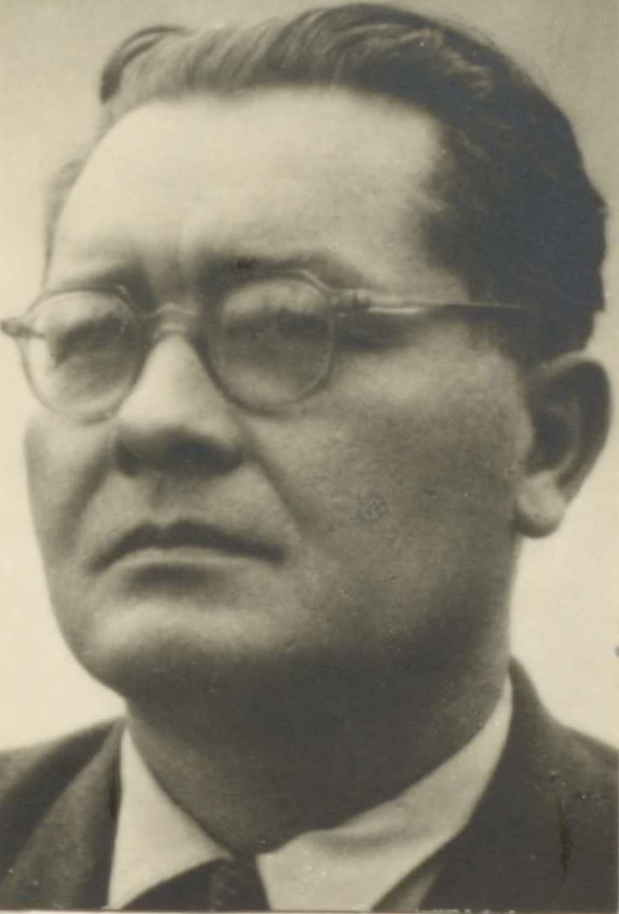
\includegraphics[width=\textwidth, height=\textheight, keepaspectratio]{173-a-ing_jaroslav_prusik}
\caption{Ing. Jaroslav Prusík z Chlumčan, člen větve Nebřeziny, jejíž část kronikářsky zpracoval (1907 – 1959)}
\label{fig:173-a-ing_jaroslav_prusik}
\end{figure}

\begin{figure}
\centering
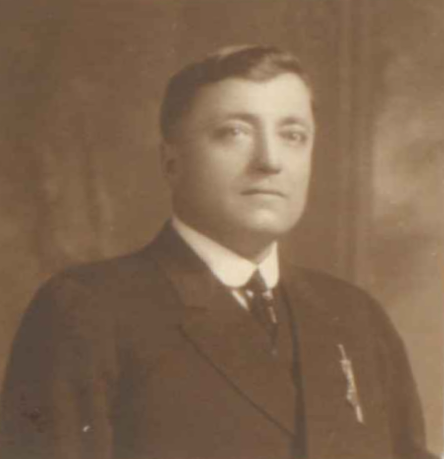
\includegraphics[width=\textwidth, height=\textheight, keepaspectratio]{173-b-josef_prusik_rodak_z_chrastovic}
\caption{Josef Prusík, rodák z Chrašťovic (1876 – 1948), čestný člen mnoha krajanských spolků v Chicagu}
\label{fig:173-b-josef_prusik_rodak_z_chrastovic}
\end{figure}

\begin{figure}
\centering
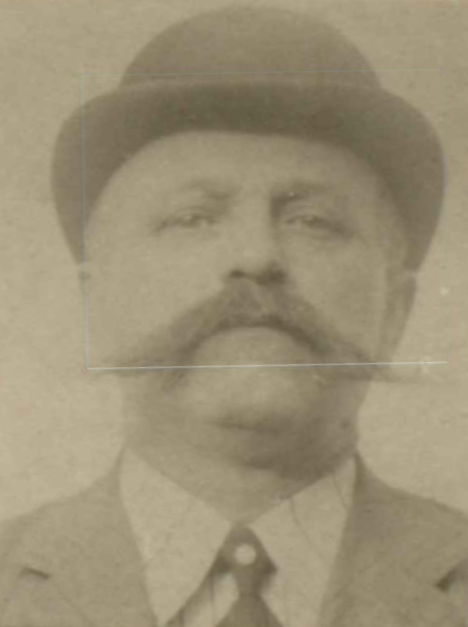
\includegraphics[width=\textwidth, height=\textheight, keepaspectratio]{173-c-karel_prusik_z_tremosne}
\caption{Karel Prusík, rodák z Třemošné, člen větve Plasy (1861 – 1938). Byl vyznamenán za spoluúčast při hašení Národního divadla při požáru 1881}
\label{fig:173-c-karel_prusik_z_tremosne}
\end{figure}

\begin{figure}
\centering
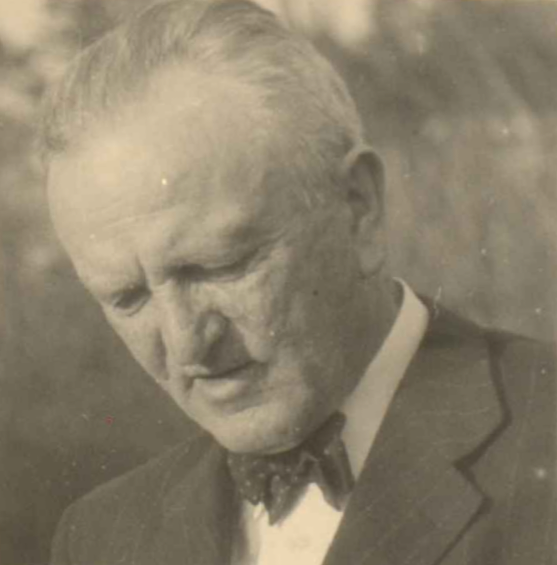
\includegraphics[width=\textwidth, height=\textheight, keepaspectratio]{173-d-mudr_blazej_prusik}
\caption{MUDr. Blažej Prusík, rodák z Výrova (1884 – 1953); byl po čtyřicet let oblíbeným lékařem v Dobříši. Jeho podpora partyzánů ve druhé světové válce byla románově zpracována}
\label{fig:173-d-mudr_blazej_prusik}
\end{figure}

 \begin{figure}
\centering
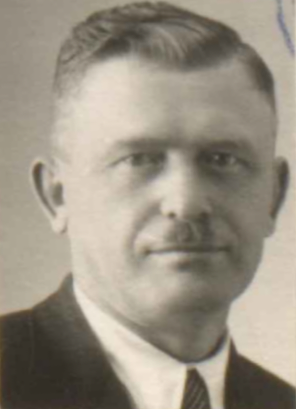
\includegraphics[width=\textwidth, height=\textheight, keepaspectratio]{173-e-josef_prusik_z_remesina}
\caption{Josef Prusík, rodák z Řemešína (1891 – 1944) byl železničním úředníkem v Kralovicích. Zahynul v koncentračním táboře v Terezíně}
\label{fig:173-e-josef_prusik_z_remesina}
\end{figure}

% str 151 @ 174
\section{Odnož Bílov - větve Sedlec}

Potomci Kateřiny Prusíkové ze Sedlce, provdané Kouklové.

1812 - 1871

Druhým dítětem Václava Prusíka, rychtáře v Sedlici a jeho ženy Rosalie roz. Fenclové z Výrova, byla dcera Kateřina. Narodila se 5. 10. 1812. Provdala se 20. 11. 1832 v potvorovském kostele za sedláka Františka Koukla z Bílova č. 8. Tím se opět dostává do této vesnice jeden člen našeho rodu. Již před Kateřinou provdaly se do Bílova některé dcery Prusíků ze Sedlice a dokonce i ke Kouklům, nebo jak se tam dosud říká "u Kymlů". Tam také byl usazen již v XVII. století kovář Václav Prusík, rodák ze Sedlice. Jeho pohnutý osud jsme již vylíčili na straně 5. Chce-li však někdo ze čtenářů těchto dějin našeho rodu viděti na vlastní oči vraha kováře Prusíka, ať navštíví Národní galerii v Praze na Hradčanech. Visí tam obraz Karla Škréty, který představuje rodinu brusičů Miseroniů, kteří působili za císaře Rudolfa II. na jeho dvoře. Ten nejmenší chlapec na obraze stal se později majetníkem hradu Krašova a v selské při zastřelil v roce 1673 Václava Prusíka.

Vesnice Bílov je položena v nejvyšší nadmořské výšce v celém bývalém okrese kralovickém. Založena byla klášterem plasským asi kolem roku 1340. V XV. století patřil Bílov pánům z Kolovrat, kteří tehdy měli Krašov a Libštejn. V roce 1480 postoupil Hanuš Kolovrat Bílov a jiné dědiny klášteru v Plasích a od těch dob, až do zrušení kláštera v roce 1785, byli plasští cisterciáci  pány nad bílovskými poddanými.

Náš venkov byl vždy velmi pobožný. V rodině Kouklů by­la však zbožnost odedávna postavena na nejvyšší místo. Kaplička vystavená v Bílově na návsi byla iniciativním dílem zvláště rodiny Kouklů a na pravé straně silnice, cestou do Potvorova stojí dosud kříž, který postavili společně František a Kateřina Kouklovi z Bílova. Na kří­ži byl vždy krásný obrázek Panny Marie, který Kateřina vždy vroucně líbávala. František Koukl, její manžel, na­rodil se 1. 8. 1811. Jeho rod je usazen v Bílově od pradávna a dříve Kouklové sluli Kymlové a také Kmínkové. Podle plasského urbáře z roku 1558, kdy ve vesnici bylo 12 osadníků, byl u tohoto gruntu č. 12 jeden lán půdy. Dnes žije v Bílově asi 150 lidí. Kateřina Kouklová rozená Prusíková zemřela v Bílově 18. 5. 1871. Její muž František zemřel za šest let po ní, 19. 11. 1877.

Kateřina Kouklová roz. Prusikova měla čtyři děti, které dospěly. Její synek Martin a dcerky Marie a Anna zemřeli v útlém věku. Nejstarším jejím synem byl Josef, který se narodil 3. 3. 1836, byl dědicem gruntu a zemřel 28. 7. 1907. Druhý syn Václav Koukl nar. 1. 9. 1841 stal se knězem a zemřel 7. 3. 1929 ve Spáleném Poříčí. Třetí syn Kateřiny byl Martin Koukl. Narodil se 17. 10. 1844, jeho teta
% str 152 @ 175
Barbora Prusíková, provdaná Levá v Sedlci, zůsta­la bezdětná, předala Martinovi svůj statek, kde pak zemřel 12. 11. 1924. Čtvrtým dítětem Kateřiny Kouklové roz. Prusíkové byla dcera Rosalie. Narodila se 4. 9. 1854 v Bílově, byla provdaná Kozová v Potvorově, kde zemřela 14. 5. 1931.

Josef Koukl v Bílově č. 8 byl nejstarším dítětem Františka Koukla a Kateřiny Prusíkové ze Sedlce. Narodil se 3. 3. 1836 a oženil se v roce 1873 s Marií Prusíkovou z Výrova. To je již čtvrtá žena z rodu Prusíků, pokud je nám známo z historie, která se provdala ke Kouklům. O ní se krátce dočtete na straně 110 u větve Výrov. Její děti podle muže zařazujeme do větve Sedlec a této odnože Bílov. Josef Koukl byl velmi nábožným člověkem, ale při tom byl přístupný moderním směrům hospodaření. Zemřel v Bílově 28. 7. 1907 a jeho žena Marie z rodu Prusíků 6. 2. 1908. A tak vlastně v půl roce ztratily děti oba rodiče.

Nejstarším synem Josefa Koukla a Marie roz. Prusíkové byl Mikuláš. Narodil se 1. 12. 1877, stal se knězem. Nejdříve byl v Nýřanech a pak na různých farách v Praze, naposled působil a žil v Praze 7. Hospodyní jeho byla příbuzná Eliška Prusíková z Horní Břízy. -Když se vrátil jeho bratr Josef, zemědělský inženýr z první světové války domů, žil pak s Mikulášem v Praze 7, Kostel­ní ulice. Mikuláš byl velmi osvícený kněz. Zemřel po­měrně mlád na chřipku 2. 9. 1926. Je pochován na Olšan­ských hřbitovech.

Druhým synem byl František Koukl. Narodil se 9. 3. 1881 a převzal doma hospodářství. Ze všech svých tří bratrů byl on nejpřísnějším katolíkem. Za ženu měl Annu Žemličkovou ze Štichovic, ale manželství zůstalo bez­dětné. Zemřel tentýž rok jako jeho bratr, kněz Mikuláš, a to 19. 12. 1926 v Bílově. Je pochován v Potvorově.

Třetím dítětem Josefa Koukla a Marie roz. Prusíkové, byl opět syn, Blažej. Narodil se 31. 12. 1883 v Bílově. Vystudoval gymnasium v Klatovech, kde jeho strýc Bla­žej Prusík byl profesorem. Po maturitě studoval na praž­ské universitě klasickou filologii, později udělal doktorát z tohoto oboru. Byl profesorem v Hustopečích na Mo­ravě, v Hodoníně, také v Táboře a nejdéle pak v Brně. I Blažej Koukl byl zaníceným katolíkem a za Lidovou stranu byl za první republiky zemským poslancem na Moravě. V roce 1925 se oženil s Antonií Vykoupilovou, rodačkou z Hodonína. Dr. Blažej Koukl miloval nadevše svůj rod a Bílov, kde se narodil. Ctil také vždy rod Prusíků, neboť jejich krev mísila se v historii velmi často s krví Kouklů. Vždyť i jeho babička a matka byly rozené Prusíkové. Blažej napsal obsáhlou historii obce Bílova a také svého rodu. Z náboženských pohnutek podnikl řa­du cest do ciziny zvláště do Itálie, Říma i do Lurd ve Francii. Zemřel v pěkném věku 83 let v Brně 7. 12. 1966.

% str 153 @ 176
Blažej Koukl měl čtyři děti. Nejstarší je Josef nar. 8. 11. 1926. Stal se knězem, krátký čas byl v Praze a pak na faře ve Stodůlkách u Prahy. Pro své pokrokové smýšlení byl zde u občanstva neobyčejně oblíben. A snad z toho důvodu musel na vyšší příkaz změnit farnost. Stal se správcem farního úřadu v Kladrubech u Stříbra, sídle někdejšího slavného benediktinského kláštera. Je tam od roku 1958 a jezdí k němu velmi často jeho matka a sourozenci. – Druhým synem Blažeje byl Václav. Narodil se 15. 4. 1928 v Brně. Počal  studovati práva, ale pro příliš vyhraněný náboženský postoj nebyl dlouho na fa­kultě. Zaučil se proto v jiném oboru a stal se úspěšným stavebním technikem u Státního statku v Kralovicích. Tam také žije v č. 82. Je ženatý a má dvě děti. Jeho synek Jan Koukl narodil se 4. 8. 1957 a dcerka Michaela je narozena 27. 5. 1963. Václav Koukl je výborným hudebníkem, hrává na varhany v kostele, jako již kdysi je­ho otec a ostatní sourozenci. Třetím synem Blažejovým byl Jan Koukl. Narodil se 23. 3. 1931 v Brně. Studoval, ale brzy byl postižen cukrovkou. Při válečném nedostat­ku léků zemřel po záchvatu 15. 8. 1945 v Bílově, kde byl na prázdninách a je pochován na hřbitově v Potvorově. Posledním dítětem Blažeje Koukla byla dcera Marie. Narodila se 28. 9. 1941. Její zbožnost, vžitá u všech Kouklů, jí nezabraňovala, aby nebyla přístupná všemu pokrokovému. Dokud byla svobodná a pracovala jako sta­vební technička, létala v letadle, jezdila autem a pod. Nyní je provdána Pospíšilová a bydlí v Brně, Merhautova č. 13/2. Marie Pospíšilová má dvě děti. Dcerka Blanka je narozena 9. 4. 1965 a syn Pavel 3. 7. 1966.

Čtvrtým synem Josefa Koukla byl Josef. Narodil se 13. 1. 1887 v Bílově, vystudoval techniku a na ní zemědělskou sekci v Praze a odešel pak do Ruska, kde jako zeměděl­ský inženýr působil ve službách na některých panstvích v moskevské gubernii. Měl velký smysl pro pokrok v ze­mědělství a jistě v Rusku dělal čest českému národu. Tam ho zastihla první světová válka a prožil i revolu­ci a občanskou válku. S naším zahraničním vojskem vrátil se pak po válce domů a byl nějaký čas úředníkem Pozemkového úřadu na Slovensku a v Praze, kde bydlil se svým bratrem Mikulášem. Když ten zemřel, zůstal krátký čas v jeho bytě, avšak po smrti svého bratra Františka odešel domu do Bílova. Oženil se s Marií Žemličkovou ze Štichovic a převzal grunt. Zůstal bezdětný. Ze všech čtyř synů Josefa Koukla a Marie roz. Prusíkové, lnul on nejvíce k našemu rodu Prusíků. Jeho zbožnost nikdy nepřecházela do fanatismu. Konec života prožíval v nejhorších hospodářských poměrech, jaké vládly zvláště po únoru 1948 na české vesnici. Zemřel v Bílově 3. 2. 1955.

Druhým dítětem Františka Koukla a Kateřiny roz. Prusíkové byl syn Václav. Narodil se 1. 9. 1841 v Bílově. Vystudoval na německém gymnasiu v Žatci, pak vstoupil do pražského semináře a na kněze byl vysvěcen 31. 7. 1867.

% str 154 @ 177
Primici slavil v Praze u sv. Josefa a slavnou mši svatou měl v Potvorově. Václav Koukl kaplanoval v Čížkově u Blovic, potom od roku 1869 do roku 1881 ve Spáleném Poříčí, pak byl 12 let farářem v Nových Mitrovicích a v roce 1893 se vrátil jako děkan do Spáleného -Poříčí, kde zemřel 7. 3. 1929 ve věku 88  let. Byl to opravdový sluha Páně a čilý až do konce života. V Nových Mitrovicích a ve Spáleném Poříčí zakoupil chudobinec. Spisovatel J. Š. Baar, bývalý kaplan poříčský, prohlásil o něm nejednou: "Jemnostpán je perla mezi kněžstvem!" Stále užíval slamníku, který mu kdysi utkala matka. Své osadníky znal dokonale, vždyť je všechny sám vychoval. Byl také horli­vým podporovatelem druhého čtenářského spolku v Če­chách, který vznikl po podobném spolku v Radnicích. Děkan Václav Koukl byl zastáncem názoru, že kněz ne­má jíti do pense, ale, že má sloužit Bohu a věřícím až do smrti. A opravdu, svíce jeho kněžského života hořela téměř 62 let. Pohřeb jeho byl velkolepý. Památce jeho přišli se poklonit z celého kraje.

Třetím dítětem Kateřiny Kouklové, roz. Prusíkové byl syn Martin. Narodil se 17. 10. 1844. Pracoval v Bílově na statku svých rodičů, a již ve svých 18. letech se oženil, když mu dala teta Barbora Levá, roz. Prusíková, své hospodářství v Sedlci č. 11. Neměla děti a nechtěla, aby její usedlost, kde se odedávna říká "u Statků" přišla do cizích rukou. Martin Koukl byl dobrým hospodářem a zvláště výborným znalcem koní, s nimiž obchodoval. Měl jedenáct dětí, ale jen šest jich dospě­lo. Martin Koukl zemřel ve věku 80 let v Sedlci, 12. 11. 1924. Nejstarším jeho dítětem byl syn Josef. Narodil se 13. 10. 1863 v Sedlci a za manželku měl Boženu Zimmerhaklovou z Podradského mlýna na Střele. Josef Koukl měl obchod v Potvorově a jednatelství pojišťovny Slavie. Ke konci života prodal Josef Koukl svůj dům s obchodem a ve staré škole zemřel pak 2. 4. 1936. Josef Koukl měl devět dětí. Dospělo jich sedm. Nejstarší byla dcera Bo­žena nar. 15. 2. 1890 v Potvorově. Byla provdána za četnického strážmistra Handla, ale Božena Handlová zemře­la již ve svých 25 letech 8. 7. 1915. I její manžel se dožil jen 41 let. Měli jediného syna Hugo Handla, nar. 24. 5. 1914 v Mladoticích. Vychoval jej pak dědeček s ba­bičkou v Potvorově. Vystudoval Vyšší průmyslovou školu strojnickou v Plzni a dnes působí na Předsednictvu vlády v Praze. Bydlí v Praze Vršovicích, Gruzinská 14. Má dvě děti. Dcera Jitřenka nar. 22. 8. 1941 je provdaná Zapletalová. Syn Ivan Handl je narozen 2. 7. 1946.

Druhé dítě Josefa Koukla byla Alžběta, naroz. 9. 11. 1891. Provdala se rovněž za četníka Jana Bulvu z Vysokého Mýta. Tam také žije v čísle 388. Alžběta Bulvová má dvě děti. Dcera Božena nar. 5. 7. 1919, je provdaná Smetanová a bydlí s matkou ve Vysokém Mýtě. Má dceru Jindřišku nar. 28. 6. 1942. Bydlí v Chrašťovicích u Pardubic č. 56a. Jitřenka Zapletalová má synka Roberta nar. 25. 4. 1968.

% str 155 @ 178
Druhé dítě Alžběty Bulvové, roz. Kouklové je syn Drahoslav. Narodil se 3. 1. 1927 v Rožnavě a dnes bydlí v Zelenči u Prahy č. 344. -Je technikem v prů­myslu v Praze. Má dvě dcery. Hanu nar. 4. 7. 1949 a Milenu Bulvovou nar. 26. 12. 1955.

Dcerka Josefa Koukla Marie, nar. 19. 1. 1895 zemřela svobodná 7. 11. 1912.

Dále byl syn Josef Koukl. Narodil se 11. 12. 1896. Nejdříve byl inspektorem pojišťovny Slavie v Kralovicích, ale později  si postavil vilu s velkou zahradou v Kralovicích a věnoval se jen ovocnářství a školkařství. Stal se vyhlášeným pomologem v kraji. Jeho zahrada je opravdu vzorem. Bydlí v Kralovicích, U soko­lovny 428. Josef Koukl má tři děti. Jeho dcera Libuše nar. 21. 11. 1926 je provdaná za lékárníka Šídla. Bydlí v Č. Budějovicích, Svatotrojická 13. Mají dvě děti. Zdeněk je narozen 4. 2. 1953 a Michal Šídl 30. 4. 1958. Syn Josef Koukl nar. 7. 11. 1927 je vedoucím elektrické rozvodny v Kralovicích. Bydlí tam s otcem. Má dvě děti - syna Josefa nar. 11. 10. 1950 a Petra nar. 30. 7. 1955. Druhý syn Josefa Koukla je Drahomír a je automechanik. Je narozen 14. 1. 1929 a bydlí rovněž ve vile svých ro­dičů v Kralovicích. Má dvě dcery. Drahomíru nar. 22. 6. 1950 a Janu Kouklovou nar. 17. 3. 1952. Dalším dítětem Josefa z Potvorova byla dcera Ludmila. Narodila se 11. 2. 1899 a také ona se vdala jako předtím již dvě je­jí sestry za četnického strážmistra Zalešáka. Žili spolu na Slovensku, později ve Vysokém Mýtě, kde Lud­mila Zalešáková zemřela 19. 9. 1960. Ludmila měla tři děti. Její dcera Miluše nar. 30. 6. 1925 je provdaná Lumerdingová. Bydlí v Chrudimi, Krocínova 511 a má dvě děti, dcery. Miluše je narozená 1. 5. 1953 a Bedřiška 20. 3. 1961. Syn Jaroslav Zalešák je narozen 1. 4. 1927 a je technickým úředníkem, bydlí v Pardubicích, Pichlova 2563. Má dvě dcerky. Danu nar. 14. 2. 1958 a Martinu Zalešákovou, nar. 29. 1. 1965. Třetím dítětem Ludmily Zalešákové byla dcera Věra. Narodila se 1. 4. 1927 a je provdaná za kon­struktéra Sigmunda ve Vlašimi. Bydlí tam ve Velíšské ulici č. 1171. Mají syna Tomáše nar. 21. 6. 1964.

Další dítě Josefa Koukla z Potvorova byl syn Vladimír. Narodil se 12. 6. 1900 a byl pracovníkem obchodního druž­stva v Plzni. Bydlí nyní v Žatci, kde žije na odpočinku v ulici Lva Tolstého č. 975/31. Má dva syny. Zdeněk Koukl narodil se 9. 7. 1926 a je úředníkem stavebního podniku v Plzni. Bydlí tam v Rejskově ulici č. 6. Má dcerku Lucii nar. 19. 8. 1965. Druhý syn Vladimíra, Dušan Koukl je strojním inženýrem. Narodil se 18. 6. 1933 v Plzni a nyní bydlí v Ostravě-Porubě, Sokolovská 1248. Má dva syny. Martina nar. 19. 4. 1961 a Jana Koukla nar. 24. 4. 1967. Posledním dítětem Josefa Koukla z Potvorova byla dcera Otilie. Narodila se 4. 5. 1904 a jako všechny tři její sestry, provdala se i ona za četnického strážmistra Frant. Komárka. Zpočátku žili na Slovensku, nyní bydlí v Praze 7, U studánky 32. Mají dvě dcery. Miluše nar. 4. 10. 1929 v Rožnavě provdala se za lékaře Pavelku. Žili nejdříve v
% str 156 @ 179
Poličce a nyní bydlí v Rýmařově, Sokolovská 42. Maji dceru Janu Pavelkovou, nar. 18. 6. 1952. Druhá dcera Jiřina narodila se 5. 6. 1932 rovněž na Slovensku a provdala se za inž. Výlupku. Nyní je roz­vedená a bydlí v Praze-Střešovicích, Hládkov 13. Má dceru Natašu nar. 29. 7. 1953.

Druhým dítětem Martina Koukla, které dospělo, byla dcera Marie. Narodila se 5. 5. 1866 za prusko-rakouské války v Sedlci č. 11. Provdala se za sedláka Juluse v Sedlici č. 14. Jejich stavení leží právě proti gruntu Prusíků, kde stála první naše kolébka. Manželství jejich zůstalo bezdětné a ještě před svou smrtí Marie Julusová, roz. Kouklová, odkázala statek své neteři Alžbětě Jánské, provdané později Chmelířové. Marie Julusová zemřela 2. 2. 1942.

Dalším dítětem Martina Koukla ze Sedlce byla Anna. Narodila se 13. 1. 1871. Provdala se za rolníka Hánu z Babiné u Plas. Naživu jim zůstaly tři děti. Marie nar. 1. 2. 1897 je provdaná Bernášková a zůstala bezdětná. Bydlí v Plzni-Doubravce, Stará cesta 14. Její sestra Alžběta nar. 7. 9. 1898 je také provdaná Bernášková a bydlí v Plzni, v domku kde její sestra. Alžběta Ber­nášková má dvě dcery. Marie nar. 26. 1. 1926 je provda­ná za inženýra Jarena a bydlí v Hořovicích č. 680. Mají dvě dcery Ivanu nar. 5. 11. 1949 a Marii nar. 3. 3. 1953. Druhá dcera Alžběty Bernáškové je Miloslava nar. 1. 2. 1932, je provdaná Weinigerová a bydlí také v Plzni-Doubravce se svou matkou. Má dceru Jindřišku, narozenou 6. 8. 1951. Třetí dcera Anny Hánové roz. Kouklové je Božena. Narodila se 30. 10. 1900 v Babině u Plas a provdala se za vlakvedoucího Molcara. Žijí nyní ve Vyklicích č. 176 u Ústí nad Labem. Má dceru Jarmilu nar. 13. 1. 1928 provdanou Tomášovou. Bydlí také ve Vyklicích. Má synka Zdeňka Tomášů nar. 3. 12. 1955. Syn Boženy Molcarové roz. Hánové je Václav. Narodil se 22. 7. 1929 a je tech­nickým úředníkem. Bydlí ve Vyklicích č. 109. Má dvě děti. Alenu naroz. 19. 9. 1955 a Václava Molcara nar. 14. 4. 1961. Anna Hánová, roz. Kouklová zemřela již 6. 11. 1906 a bylo jí tedy pouze 35 let. Její manžel se ještě podruhé oženil.

Třetí dcerou Martina Koukla ze Sedlice byla Josefa. Narodila se 12. 8. 1875. V den svých dvacátých narozenin provdala se za rolníka Václava Jánského v Potvorově č. 45. Po statku se tam říkalo "u Kuříčků". Josefa Jánská měla řadu dětí, které vždy k sobě velmi lnuly. Nebývá to vždy tak v rodinách, zvláště, když jde o devět sourozenců. Josefa Jánská, roz. Kouklová zemřela v Pot­vorově 11. 1. 1949.

Nejstarší její dcera byla Alžběta. Narodila se 19. 11. 1896 v Potvorově a jí odkázala bezdětná teta Marie Ju­lusová, statek v Sedlci č. 14. Alžběta Jánská provdala se za rolníka Tomáše Chmelíře z Tatiné a hospodařili spolu v Sedlci. Měli tři děti, ale osud nebyl této rodině
% str 157 @ 180
vždy příznivě nakloněn. Zvláště se to týká je­jich syna Jaromíra Chmelíře. Narodil se 4. 4. 1924 a po květnu 1945 byl značně postižen novými politickými poměry. Dnes bydlí v Plzni-Slovanech, Schwarzova 50. Má dvojčata, dcerky Michaelu a Dagmar nar. na štědrý den v roce 1964. Dostali tedy pěknou vánoční nadílku. Druhým dítětem Alžběty Chmelířové je dcera Jarmila. Je narozena 27. 12. 1925 a provdaná Václavíková v Kory­tech č. 42 u Plas. Má dvě děti. Hanu nar. 14. 7. 1956 a Václava Václavíka nar. 16. 3. 1958.

Třetím dítětem Alžběty Chmelířové roz. Jánské, je syn František. Narodil se 2. 12. 1931 v Sedlci č. 14 a zůstal doma. Má synka Petra nar. 5. 9. 1961. Pracuje v JZD a když se podívá na protější opuštěný statek Prusíků, může si jistě zafilosofovat. Vždyť přes 350 let žil zde rod Prusíků, k němuž také patří, byl na prvním místě v obci, kde bývala také rychta a dnes to vše patří jen vzpomínkám. Další dítě Josefy Jánské byla dcera Marie. Narodila se 25. 11. 1898 a provdala se za rolníka Fran­tiška Nezbedu v Potvorově č. 49. Měla dvě děti. Její syn Josef Nezbeda nar. 12. 5. 1928 má dvě děti. Synka Jo­sefa nar. 22. 6. 1957 a dceru Libuši Nezbedovou nar. 8. 1. 1961. Druhá dcera Marie, nar. 28. 6. 1929 provdala se za zemědělce Havlíka do blízké Bukoviny č. 10. Mají dvě děti. Václava nar. 13. 5. 1954 a Marii nar. 26. 6. 1957. Dalším dítětem Josefy Jánské roz. Kouklové byl syn Mi­kuláš. Narodil se 1. 7. 1903 a ujal se po rodičích rod­ného statku v Potvorově. Zemřel 24. 11. 1958. Mikuláš Ján­ský měl dva syny. Václava naroz. 12. 9. 1933, který zůstal doma. Je předsedou JZD v Potvorově. Má dvě děti. Dcerku Zdenku Jánskou naroz. 20. 8. 1962 a syna Pavla nar. 7. 9. 1965. Druhý syn Mikuláše Jánského Jaroslav narodil se 20. 2. 1935. Pracuje a žije dnes v Ostrově nad Ohří, ul. Zápotockého 1184/20. Má dvě děti, Jitku Jánskou nar. 25. 11. 1963 a Libora nar. 25. 4. 1967.

Dalším dítětem Josefy Jánské byla dcera Božena. Narodila se 6. 7. 1905, byla provdaná Bestahovská, ale manželství se nevydařilo. Je bezdětná a žije v Potvo­rově č. 35. Dále měla Josefa Jánská syna Bohuslava. Narodil se 15. 4. 1900. Vyučil se zámečnictví a pracoval v Lounech. Dnes bydlí v Jimlíně č. 168 u Loun. Měl jediné dítě, syna Bohuslava nar. 25. 9. 1928. Bohuslav Jánský je plukovníkem a bydlí v Sokolově, Březová 177. Má dcerku Hanu nar. 7. 3. 1958.

Další dcerou Josefy Jánské roz. Kouklové byla Anna. Narodila se 6. 1. 1902 a provdala se za policejního inspektora Durdíka. Žili v Praze a vdova Anna Durdíková bydlí na Petřinách v Praze 6, čp 1788. Má jedinou dce­ru Marcelu, provdanou za chemika Hacha. Marcela se narodila 22. 7. 1931. Pracuje ve zdravotnictví, Anna Durdíková patří k těm, kdož mají zvláštní pochopení pro rodinná pouta a stále je udržovat. Další dítě Josefy Jánské, je Růžena. Narodila se 25. 2. 1907 v Potvorově a provdala se za zemědělce a nadšeného varhaníka Slacha. Bydlí v Potvorově č. 39. Má dvě děti. Její syn Blažej Slach nar. 26. 1. 1935 pracuje a bydlí v Ostrově nad Ohří,
% str 158 @ 181
Jáchymovská č. 1134. Má dvě děti. Blažeje nar. 2. 2. 1962 a dcerku Janu Slachovou nar. 7. 8. 1965. Druhé dítě Rů­ženy Slachové je dcera Marie. Narodila se 13. 2. 1940 a je provdaná Hoťková v Plzni. Má dvě dcerky. Václavu nar. 6. 10. 1962 a Jaroslavu nar. 30. 6. 1967. Dalším synem Josefy Jánské je Václav. Narodil se 6. 9. 1908 v Potvorově. Pracuje a bydlí v Chomutově, Šafaříkova 21. Václav Jánský má dvě děti. Dcera Libuše nar. 19. 12. 1944 je provdaná Moravcová a má synka Oldřicha  nar. 21. 4. 1964. Další syn Václava Jánského je Václav. Narodil se 31. 5. 1951. Bydlí s rodiči v Chomutově. Posledním dítětem Josefy Jánské roz. Kouklové byl syn Ladislav. Narodil se 13. 6. 1916 a vyučil se drogistou. Nyní žije v Žíhli č. 68. Má jediné dítě, synka Ladisla­va nar. 9. 8. 1950. Studuje lesnictví.

Předposledním synem Martina Koukla byl František. Narodil se 4. 7. 1878 v usedlosti "u Statků" v Sedlci. Stal se dědicem rodného gruntu. Měl jedinou dceru Marii. Narodila se 18. 1. 1909 a provdala se za Václava Kronďáka z Trojan. Zde oba po Františku Kouklovi hospodaří, ovšem dnes v JZD. Mají tři děti. Dcera Jarmila je provdaná Sou­kupová v Potvorově č. 38. Narodila se 28. 8. 1938 v Sedlci. Má tři děti. Jiřího nar. 7. 3. 1958, Marii nar. 13. 9. 1959 a Ivanu nar. 13. 9. 1964. - Druhou dcerou manželů Kronďákových je Marie. Narodila se 30. 9. 1939 a dnes žije provda­ná Vopatová v Žebnici č. 28. Má dvě dcery. Anna je na­rozená 9. 11. 1960 a Marie 21. 10. 1962. Syn Václav Kronďák, nar. 13. 5. 1941 zůstal doma v Sedlci. Má dvě děti. Václavku nar. 28. 3. 1964 a Pavla nar. 6. 6. 1967.

Posledním dítětem Martina Koukla byl syn Augustin. Narodil se 18. 8. 1881 v Sedlci. Stal se sládkem a žil pak 14 let v Rusku. Jeho ženou byla Lotyška a dlouho žili v městě Grozném na Kavkaze. Po první světové válce vrá­tili se oba do naší republiky, Augustin Koukl byl pak ředitelem pivovarského skladu v Kožlanech. Manželství bylo bezdětné. Když Augustin odešel na pensi, zakoupi­li si se svou ženou domek v Kralovicích, ale později se uchýlili do Domova přestárlých v Liblíně. Tam Augustin Koukl zemřel 27. 7. 1958. Když býval v Rusku zasílal ra­dy svému příbuznému inž. Josefu Kouklovi z Bílova, kte­rý pak také za ním odjel do Ruska.

Tím je skončeno líčení o životě potomků Martina Koukla ze Sedlce, který se narodil také ještě za doby roboty, v Bílově.
Posledním dítětem Kateřiny Kouklové  rozené Prusíkové byla dcera Rosalie. Narodila se 4. 9. 1854 a provdala se v roce 1872 za rolníka Josefa Kozu v Potvorově 41. Rosalie Kozová roz. Kouklová byla neobyčejně pracovitou, zbožnou a bystrou ženou. Ona byla učiněným historiografem Potvorova a v jejím zápisníku byly zachyceny všechny události obce i lidí za více než padesát let.

% str 159 @ 182
Bílovská rodačka Rosalie Kouklová, pak provdaná Kozová v Potvorově byla tak zbožná, že kdykoliv slyšela bíti hodiny, nikdy neopomenula říci: "Pane Ježíši Kriste, hodi­na již odbila, hrobu mému se blíž přiblížila. Prosím Tě, až udeří ta má poslední, dejž mých hříchů, odpuštění!" Rosalie Kozová v Potvorově měla sedm dětí, které dospě­ly. Kdykoliv zde vyslovujeme "děti dospěly" ,myslíme tím, při citování děti, které dosáhly alespoň věku deseti let. Bývaly časy, kdy rodiče měli i patnáct dětí, ale z nich často jen dvě až tři děti dosáhly deseti let a delšího věku.

Kdybychom citovali všechny narozené děti členů našeho rodu, které jsme našli v matrikách, pak by asi rozsah tohoto díla byl nejméně dvojnásobný. Výčet tento by však nikomu nic neříkal. Vždyť je dnes dobře známo, jaká straš­ná úmrtnost dětí byla v dřívějších dobách. Rosalie Kozová měla dvě dcery a pět synů. Zemřela jako vážená občanka Potvorova 14. 5. 1931.

Nejstarší její dítě byla Marie. Narodila se 22. 2. 1875 v Potvorově. Vdala se za Václava Urbana a hospodařili spolu v usedlosti č. 61 v Potvorově, kde se říká "u Ur­banů". Marie Urbanová roz. Kozová měla dceru Marii nar. 15. 9. 1894, která zemřela svobodná 25. 6. 1949. Její syn Josef Urban, narozený 13. 3. 1896 hospodařil v Potvoro­vě v č. 69. Josef Urban zemřel v roce 1943. Měl jediné dítě, syna Václava nar. 26. 8. 1931. Ten pracuje v továrně TOS v Lubenci. Další dítě Marie Urbanové roz. Kozové byl František. Narodil se 9. 12. 1898 a zůstal doma v č. 61. Má dvě děti. Dcera Marie je narozena 17. 11. 1933 a je provdaná Kloučková v Potvorově č. 4. Má dva chlapce, Jarosla­va Kloučka nar. 26. 4. 1957 a Milana nar. 4. 9. 1960. Syn Františka Urbana, Václav nar. 9. 9. 1938 žije v Potvorově a je svobodný.

Marie Urbanová roz. Kozová byla nejstarším dítětem Rosa­lie a zemřela jako poslední ze svých sourozenců 10. 11. 1963.

Dále měla Rosalie Kozová, roz. Kouklová, syna Josefa. Narodil se 24. 2. 1877. Vyučil se řeznictví. Měl v Potvo­rově u svého hostince velké polnosti. Josef Koza znač­ně zbohatl i z obchodu koňmi a v roce 1923 zakoupil si velkostatek Pohvizdy u Žíhle. Měl dvě dcery. Starší Božena nar. 28. 12. 1905 byla provdaná Řebíčková a se svým manželem vedli pak velkostatek Pohvizdy. Měli jediného syna Karla, nar. 16. 9. 1928. Jako všichni, kdož měli vět­ší majetek, špatně dopadli po květnu 1945. Z Pohvizd se vystěhovali a Karlu Řebíčkovi byly ztíženy studie. Dnes je stavebním technikem a bydlí v Praze-Spořilově II, Sídliště B 2, č. 2516. Má dceru Blanku nar. 5. 5. 1965. Matka jeho Božena Řebíčková žila v Kralovicích, ve Stříbře, také nějaký čas po ovdovění v Bukovině a po nekonečném putování bydlí nyní blíže svého syna v Pra­ze, na Spořilově.

% str 160 @ 183
Druhou, dcerou Josefa Kozy byla Marie, která se narodi­la 7. 4. 1911 v Potvorově a vdala se za majitele velkostat­ku Vysoká Libyně, Koulu. Hospodařili spolu v této obci, ale za okupace, když byla zabrána, odešli do Obytců u Klatov,  kde měli pronajatý dvůr. Po válce se sice vrátili na chvíli do Vysoké Libyně, ale pak také přišli o vše a bydleli nakonec v menším domku u hřbitova v Kra­lovících. Marie Kouklová zemřela náhle 15. 1. 1968. Měla jednu dceru, Jaroslavu nar. 6. 8. 1935. Je provdaná Janko­vá a bydlí v domku v Kralovicích, Tyršova ul., kde žila se svou matkou. Jaroslava Janková má dvě děti. František je narozen 7. 2. 1956 a dcera Jaroslava 29. 5. 1958.

Dalším dítětem Rosalie Kozové byl František. Narodil se 14. 3. 1879 a přiženil se do Bukoviny č. 1, kde se říkalo "u Masopustů". Je zajímavé, že do tohoto stave­ní se v I. polovině XVIII. století provdala ze Sedlice Anna Prusíková. František Koza zemřel 17. 2. 1955. Jeho syn František nar. 29. 4. 1914 je svobodný a žije v Bukovině č. 1 jako člen JZD. Sestra jeho Anna provdaná Sebránková narodila se 16. 5. 1916 a bydlí také v Buko­vině č. 1. Má dvě děti. Je to syn Jaroslav nar. 15. 9. 1952 a dcera Květoslava Sebránková nar. 6. 2. 1955. Dále měl František Koza v Bukovině syna Václava. Narodil se 3. 6. 1918 a dnes žije v Málkovicích č. 3 u Stříbra. Je zaměstnancem státního statku. Má syna Pavla Kozu, nar. 24. 2. 1949. Dcera Františka Kozy Marie, nar. 3. 6. 1920 v Bukovině provdala se za Františka Slacha do Bílova 29 a měla tam s ním sedm dětí. O nich jsme již psali na straně č. 116 u odnože Výrov II.

Dalším synem Rosalie Kozové byl Václav. Narodil se 6. 5. 1881, hospodařil v Potvorově č. 41 na rodném statku. Zemřel tam 3. 10. 1951. Jeho syn Václav nar. 31. 8. 1911 žije v téže usedlosti v Potvorově a je svobodný. Další syn Blažej Koza nar. 7. 1. 1913 žije v Praze 3-Žižkov, Dali­milova 19. Je úředníkem národního výboru. Je také svobodný. Třetí syn Václava Kozy, Bohuslav narodil se 31. 8. 1914. Dnes je ředitelem státního statku v Kralovicích a bydlí tam tř. Rudé armády 529. Má dvě děti. Dcera Olga je narozena 16. 1. 1947 a syn Václav 6. 7. 1952. –Poslední syn Václava Kozy z Potvorova je František, naroz. 1. 6. 1917 je také dosud svobodný a bydlí v Potvorově.

Dalším dítětem Rosalie Kozové byl Antonín Koza. Narodil se 3. 6. 1883 a padl ve světové válce v roce 1917.

Dcera Rosalie Kozové, opět Rosalie narodila se 11. 8. 1889. Provdala se za rolníka Vopata z Řemešína. Měla dceru Marii, která se narodila 22. 11. 1924 a provdala se za rolníka Buška do Kopidla č. 7. Má dva syny, Jaroslava nar. 17. 10. 1958 a Josefa nar. 1. 5. 1963. Rosalie Vopatová zemřela 19. 7. 1932.

Posledním dítětem Rosalie byl Pavel Koza. Narodil se 5. 6. 1893 v Potvorově a padl brzy na začátku světové války na ruské frontě v Haliči 20. 11. 1914.

% str 161 @ 184
Rosalie Kozová, narozená Kouklová měla, jak jsme Vám vylíčili, sedm dětí, ale osudy přemnohých se vyvíjely špatné. Její syn Josef, který tak zbohatl a obě jeho dcery, které měly za muže velkostatkáře, v důsled­ku revolučních přeměn zcela zchudly. Dva její synové Antonín a Pavel padli ve světové válce a ze čtyř dětí jejího syna, Václava Kozy,  zůstali tři synové svo­bodní. Dnes tedy žije potomků Rosálie velmi málo.

Tímto vyprávěním jsme poodhalili poněkud roušku nad dosud neznámými událostmi ze života potomků Kateřiny Kouklové rozené Prusíkové ze Sedlce. Z celého rodu Prusíků, pokud je nám známo z historie, stalo se šest členů knězi. A právě z rodiny Kateřiny Kouklové byl jich největší počet, celkem tři. Zbožnost v této rodině byla vždy na nejpřednějším místě. Kateřina Kouklová roz. Prusíková přestože měla jen čtyři děti a z těch ještě jeden se stal knězem, zanechala po sobě 170 p0t0mků z toho dnes již 27 mrtvých.

% TODO foto

% str 161+1 @ 185
\begin{figure}
\centering
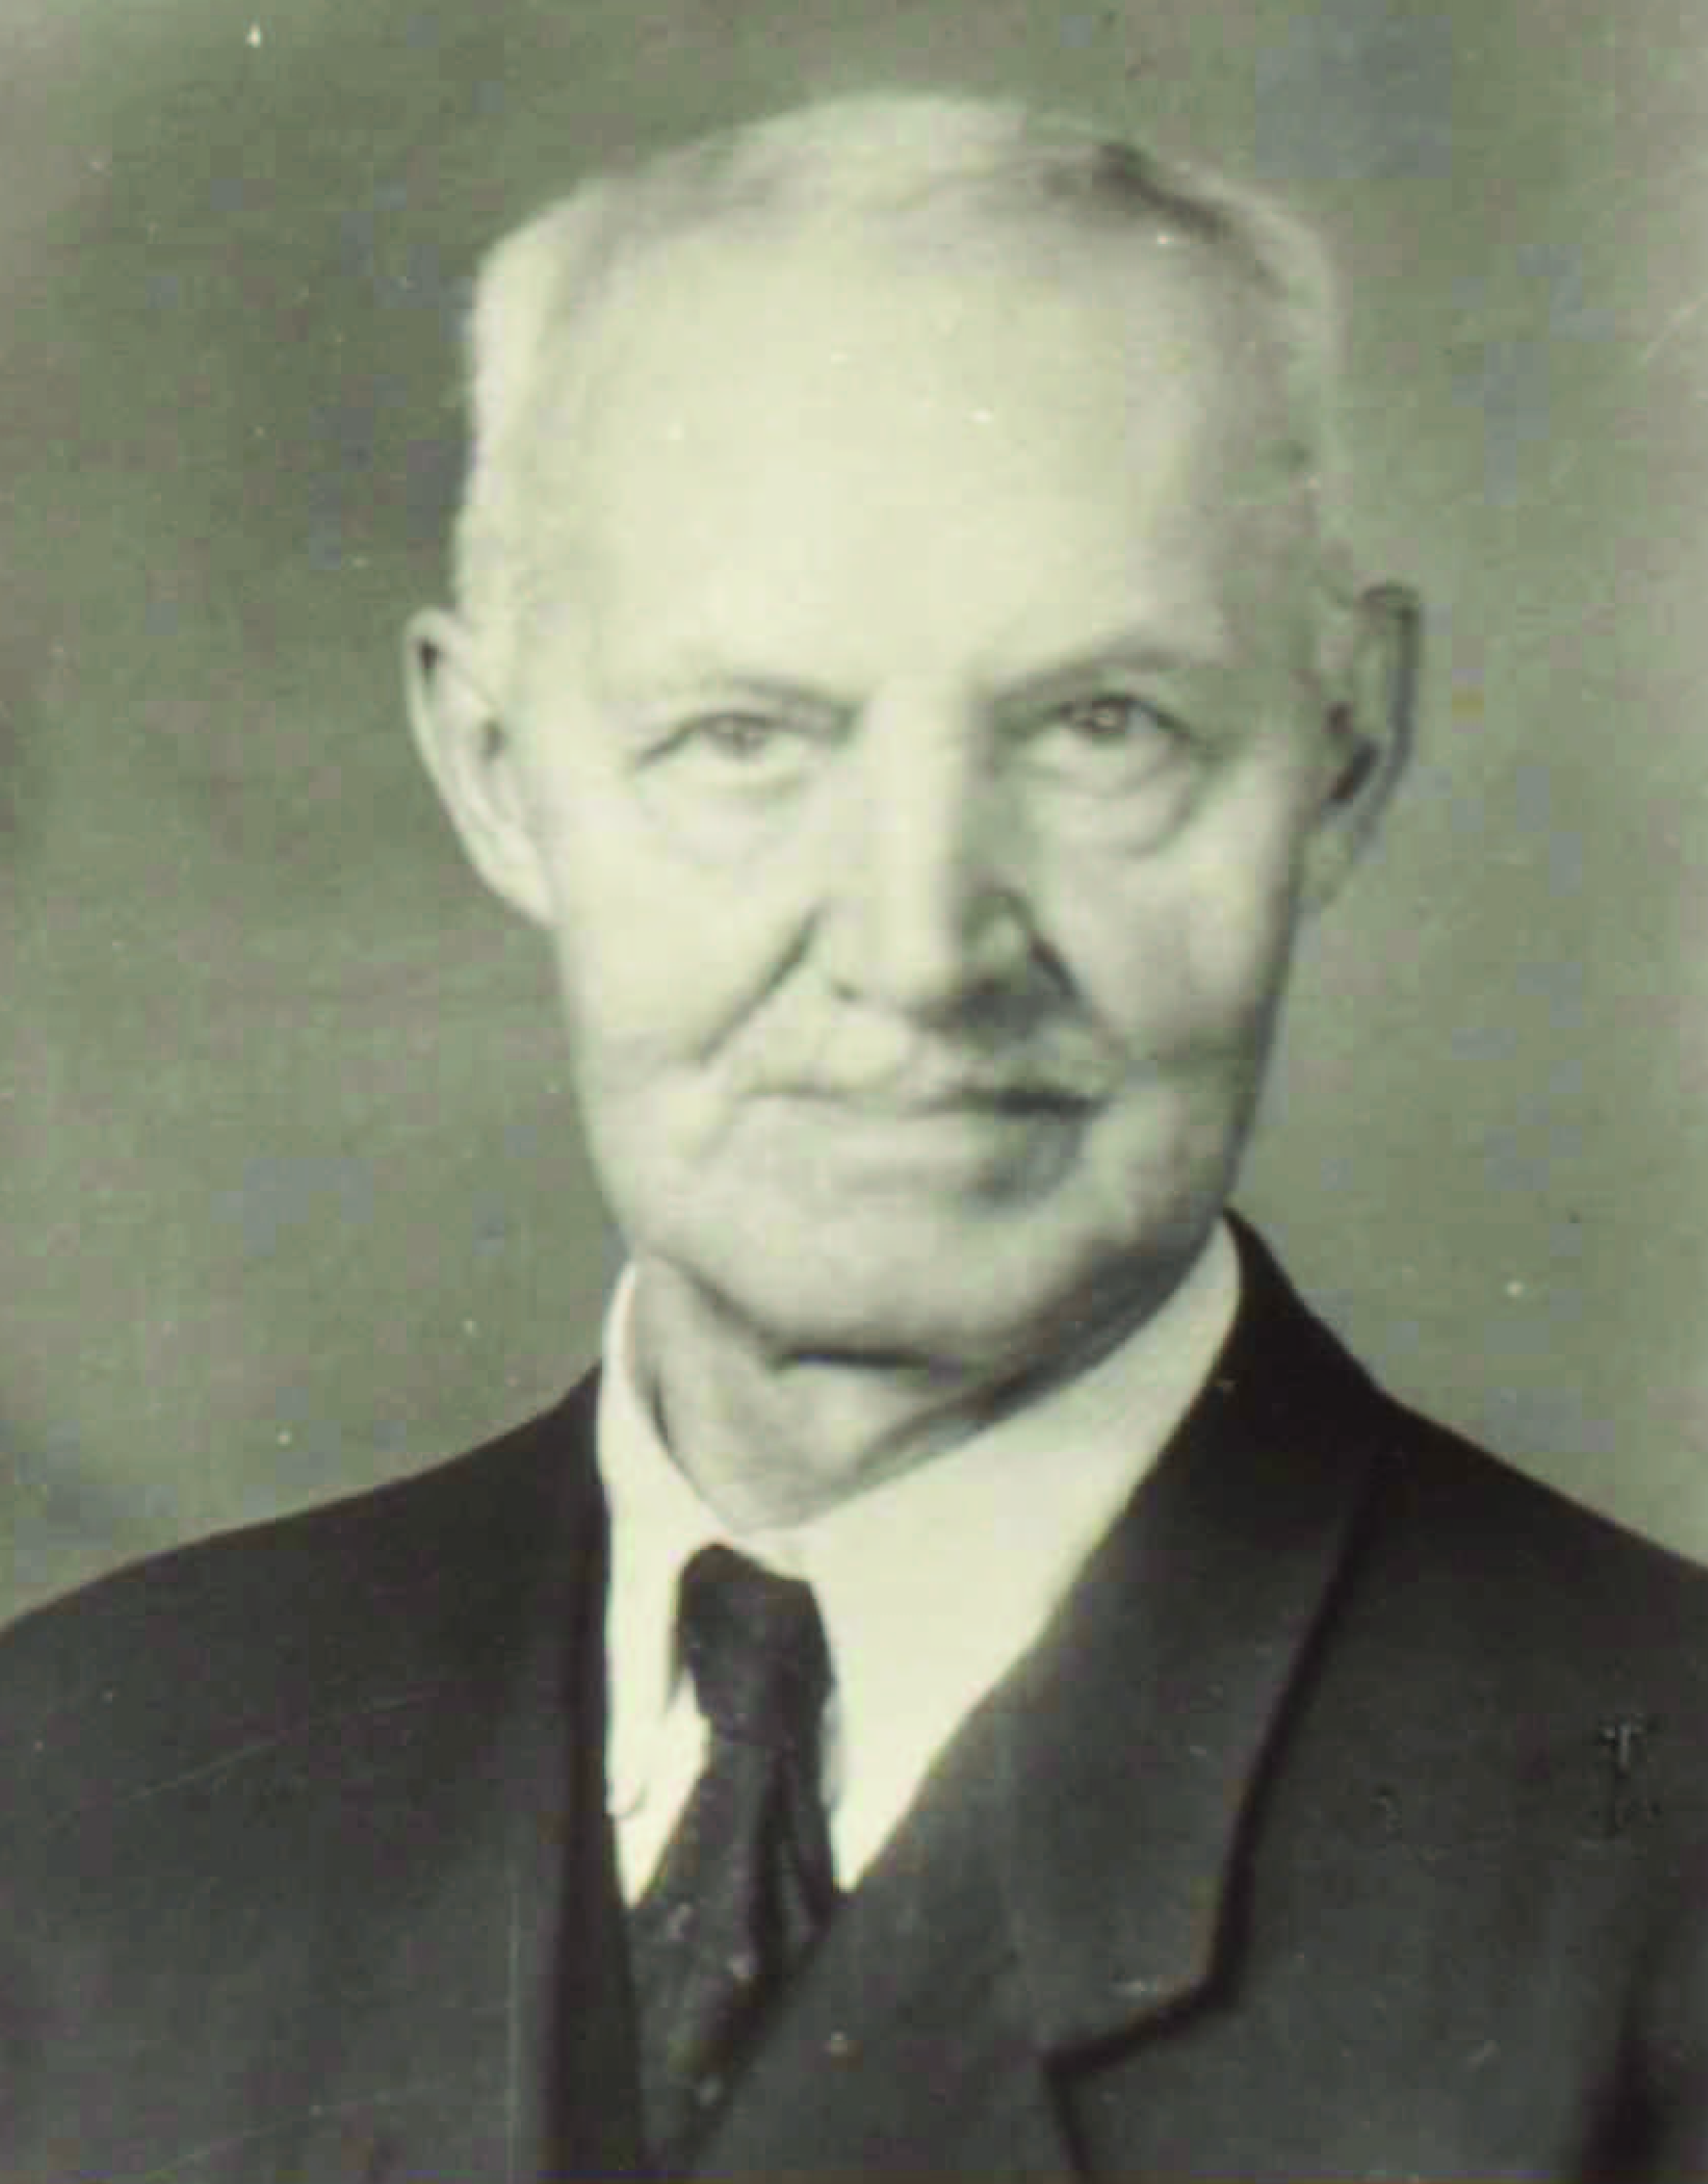
\includegraphics[width=\textwidth, height=\textheight, keepaspectratio]{184-prof_dr_blazej_prusik}
\caption{Profesor dr. Blažej Prusík Koukl (1883 – 1966), rodák bílovský, člen větve Sedlec. Sepsal podrobnou historii svého rodu i rodiště, k němuž lnul vždy velkou láskou}
\label{fig:184-prof_dr_blazej_prusik}
\end{figure}


% str 162 @ 186
\section{Odnož Šípy - větve Sedlec}

Potomci Tomáše Prusíka rodáka ze Sedlce, usazeného v Šípech u Čisté.

1822 - 1862

Rychtář Václav Prusík se svou ženou Rosalií v Sedlci měli čtvrté dítě, syna Tomáše. Před ním narodila se v gruntě č. 4 v Sedlci dcera Barbora 28. 9. 1816. Vdala se v roce 1840 za sedláka Vojtěcha Levého v Sedlci č. 11 a zemřela bezdětná 11. 11. 1887. Její hospodářství, jak jsme již o tom psali, převzal ještě dlouho před její smrtí, její synovec Martin Koukl z Bílova.

Tomáš Prusík narodil se v Sedlci 1. 12. 1822. Oženil se s Rosalií Šimandlovou z Potvorova, která se tam naro­dila 20. 5. 1829. Určitý čas hledali, kde by se zakoupi­li. A tu se jim v roce 1852 naskytla příležitostná kou­pě v podobě usedlosti č. 5 v Šípech u Čisté. V této usedlosti do té doby hospodařili manželé Foldovi. Zatím je nejasné, proč 17. 12. 1857 předal smlouvou za 400 zla­tých Tomáš Prusík svou polovinu své manželce Rosalii. Snad proto, že již v té době byl nemocen.

Vesnice Šípy ležící blízko památného hradu Krakovce, kde Jan Hus pobýval před odchodem do Kostnice, patřívala odedávna ke královskému hradu Křivoklátu. V době Husova pobytu na Krakovci, byla obec Šípy majetkem hostitele Husova pana Jindřicha Lefla z Lažan. Později byla zde vrchností rodina Kolovratů. Nakonec patřily Šípy panství chřičskému. Po třicetileté válce bylo v Šípech deset osadníků. Dnes tam žije asi 250 lidí.

Tomáš Prusík měl se svou manželkou Rosalií čtyři dcery. Synek Josef nar. 1855 zemřel v Sedlci, rodišti Tomášově v roce 1859. Nejstarší dcera byla Barbora nar. 17. 10. 1853 v Potvorově, rodišti své matky. Byla provdaná Slabá a dostala pak grunt po rodičích. Zemřela poměrně mla­dá v Šípech 29. 2. 1892. Druhá Marie, narodila se 24. 12. 1857 také v Potvorově, ačkoliv již rodiče hospodařili v Šípech. Bývalo to tak často, že rodička jela ke své mat­ce před svou těžkou hodinkou. Marie se provdala za sedláka Zikmunda do Pavlíkova u Rakovníka a tam zemřela 7. 9. 1910. Třetí dcerou Tomáše Prusíka byla Anna, nar. 5. 5. 1860 v Šípech a byla zpočátku provdaná v Bělbožicích a pak v Břežanech jako Fryčová. Zemřela tam 20. 12. 1938. Poslední byla Josefa nar. 30. 8. 1861 v Šípech. Byla provdaná Gubová a zemřela 11. 4. 1943 v Chomutově.

Tomáš Prusík neměl však dlouhý život. Zemřel na vodnatelnost, jak je v matrice psáno, což podle našich dneš­ních pojmů je asi rakovina, 14. 6. 1862 v Šípech. Vdově Rosalii bylo tedy jen 33 let a vdala se za rok za Voj­těcha Loose z Hlinců. Z tohoto druhého manželství měla dceru Julianu, později provdanou Spurnou. Rosalie Loosová dříve Prusiková zemřela 21. 10. 1884 v Šípech.

% str 163 @ 187
První dcerou Tomáše Prusíka a jeho ženy Rosalie byla Barbora. Narodila se 17. 10. 1853 v rodišti své matky Potvorově, v roce 1878 se provdala za Antonína Slabého z Miličova, který se do Šípů přiženil. Měli spolu šest dětí, dlouho však spolu nežili. Barbora Slabá roz. Prusíková zemřela p0 potratu dne 29. 2. 1892. Děti jejich byly dcery, Antonie, Anna, Marie, Františka a Anežka a syn Antonín. Vdovec Antonín Slabý se znovu oženil a měl pak ještě šest dětí. Antonín Slabý býval dlouhá leta starostou v Šípech.

První dítě Barbory Slabé, roz. Prusíkové byla dcera Antonie. Narodila se 2. 12. 1879 v Šípech. Provdala se za sedláka Herinka do Zavidova u Rakovníka. Byla to velmi rázná a pracovitá žena a ona se hlavně také starala, aby grunt, kde se narodila v Šípech dostal její bratr Antonín z prvního manželství otcova. Antonie Herinková, roz. Slabá měla jedinou dceru Annu. Antonie Herinková zemřela v Zavidově 24. 5. 1956. Její dcera Anna narodila se 11. 4. 1905 a je provdaná za rolníka Beneše, vzdáleně spříz­něného s bývalým presidentem republiky Dr. E. Benešem. Anna Benešová měla tři děti. Nikdo z nich nezůstal doma a sama s manželem je členem JZD. Nejstarším dítětem Anny Benešové je syn Květoslav. Narodil se 28. 8. 1925, vystudoval technický odbor a je dnes profesorem průmyslo­vé školy v Bratislavě. Na Slovensko se dostal proto, že má za ženu Slovenku, která po druhé světové válce se přistě­hovala z Maďarska. Bydlí v Bratislavě - Sídliště Strkovec, Haburská 7. Mají tři děti. Petra nar. 28. 9. 1954, Květoslava nar. 3. 6. 1952 a dceru Darinu Benešovou nar. 16. 8. 1959. Druhým dítětem je Libuše. Narodila se 24. 1. 1927 a je provdaná Vrabíková. Bydlí v Podbořanech, Husova 718 a s manželem pracují v zemědělském oboru. Mají dceru Jitku, nar. 14. 10. 1948, druhá dcera je Libuše nar. 27. 1. 1951.

Třetím dítětem Anny Benešové ze Zavidova je dcera Vědunka. Narodila se 30. 3. 1929 a je provdaná v Rakovníce, ul. Na sekyře. Má dvě děti, syny Milana nar. 1. 12. 1952 a Karla Ziku nar. 18. 2. 1956.

Druhou dcerou Barbory Slabé roz. Prusíkové byla Anna. Narodila se v Šípech 24. 4. 1881. Provdala se za obuvníka Kouteckého v Žatci. P0 okupaci pohraničí žila jako vdova u své dcery v Praze-Hostivaři. Zemřela 5. 3. 1950.

Dcera Anny Koutecké, roz. Slabé, Elfrida narodila se 5. 3. 1907 v Žatci. Je provdaná Hřavová a bydlí v Praze-Hostivaři ve vlastní vilce ulice Pod stanicí 660. Její muž byl zaměstnancem ČSD. Elfrida Hřavová má pět dětí. Syn Jaromír Hřava nar. 10. 4. 1929 je svobodný. Je technickým úředníkem. Druhý Jan nar. 24. 12. 1930, pracuje v automobilce AZKG. Má dcerku Janu Hřavovou nar. 19. 1. 196o. Další syn je Jaroslav Hřava. Narodil se v 27. 4. 1940 a je strojvedoucím. Čtvrtý syn Jiří nar. 24. 6. 1942 pracuje v telekomunikačním ústavu v Praze Strašnicích. Má dceru Renatu nar. 4. 2. 1965. Dcera Anna nar. 27. 12. 1947 je provdaná Roubalová. Má syna Daniela nar. 7. 3. 1967. Bydlí s rodiči v Hostivaři.

% str 164 @ 188
Další dcerou Barbory Prusíkové provdané Slabé v Šípech byla dcera Marie. Narodila se v Šípech 26. 5. 1884. Provdala se za obuvníka Makovského a se sestrou Františkou odjela v roce 1908 do Ameriky. Žila tam hlavně ve státě Montana v městě Great Falls. Měla jediné dítě, dcerku a brzy po porodu zemřela. Šla za štěstím za moře, ale užila ho pramálo. Zemřela již 26. 3. 1910. Jediná je­jí dcera Anna narodila se 5. 3. 1910 a za tři týdny osi­řela po matce. Dnes je provdaná Willemsová a je ošetřo­vatelkou v sanatoriu. Je bezdětná. Žije v místě Springville v Kalifornii. Má tam svou poštovní schránku tzv. PO BOX 655.

Čtvrtou dcerou Barbory Slabé roz. Prusíkové byla Fran­tiška. Narodila se 6. 4. 1886. Jako její sestra Marie, také ona viděla svůj šťastný přelud v Americe. Jejím manželem byl obuvník Makovský, jehož bratr byl manže­lem její sestry Marie. Františka Makovská také dlouho žila ve státě Montana v USA. Tento kraj je velmi horna­tý a lesnatý a je zde i přírodní park USA se všemi svými romantickými půvaby. Františka Makovská měla čtyři dcery. Často vzpomíná na domov, který v Šípech dlouho neužila. Nyní již velmi churaví a žije v domově přestárlých v městě Marysville ve státě Washington. I když je tam o ní dobře postaráno, dcery na ní nezapomínají a velmi často ji navštěvují.

Nejstarší dcerou Františky Makovské rozené Slabé je Eliška. Narodila se 10. 11. 1910 a byla poprvé vdaná Knoxová. Z tohoto jejího prvního manželství má syna Kennetha. Narodil se 2. 3. 1930. Je letcem a žije dnes ve městě, kde je jedna z největších leteckých základen USA, v městě Tacoma u Tichého oceánu, 1317, 116th Street. Má dvě dcerky Zu­zanu nar. 10. 6. 1956, Kateřinu 11. 3. 1961 a synka Kennetha, nar. 12. 5. 1958. Další i dítěten Elišky Knoxové je Kateřina. Je narozená 18. 2. 1931 a žije dnes jako provdaná Greerová v městečku Simma ve státě Montana. Má 4 dcery a 1 synka. Jména dcer jsou: Barbora nar. 6. 2. 1950, Sharon nar. 28. 7. 1952, Jayne nar. 21. 10. 1955 a Kateřina nar. 14. 4. 1957. Syn se jmenuje James (Jakub). Je narozen 31. 5. 1960. Podruhé je Eliška Makovská provdaná Phillipsová. Z tohoto manželství má dceru Marilyn, nar. 21. 8. 1938. Je dnes provdaná Wangsmová. Její manžel je norského původu. Bydlí ve státě Washington v městě Marysville, 8220, 53rd drive. Marilyn Wangsmo má dvě děti, dcerku Janis nar. 13. 7. 1960 a synka Jay nar. 21. 2. 1962. Eliška Philipsová nar. Makovská žije v Marysville, 9320 Pacific Highway.

Druhou dcerou Františky Makovské rozené Slabé je Libuše. Narodila se v městě Coffee Creek ve statě Montana 2. 10. 1912. Je provdaná za obchodníka Vance. Libuše nebo po americku Libby má dva syny. Allen Vance nar. 19. 4. 1935 má dva hochy Allena nar. 17. 11. 1956 a Kevina Vance nar. 24. 8. 1959. Bydlí v Marysville, Route 2, Box 949 ve státě Washing­ton. Jeho bratr Gary Vance narodil se 24. 7. 1939 a žije také v městě Marysville, 1889, Liberty Lane. Gary má 4 děti. Dcera Wendy je narozená 17. 12. 1959, druhá Jerry nar. 28. 1. 1961, pak je syn Guy Vance nar. 17. 6. 1962 a třetí dcerka
% str 165 @ 189
Karen Vance nar. 14. 9. 1963. Libuše Vanceová rozená Makovská bydlí jako její syni také v Marysville ve státě Washington v USA.
Když byli upozorněni tito členové rodu Prusíků, i když již nemají povodní jméno, že v jejich státě je v pohoří Cashmere Grags jeden strmý vrchol pojmenován Prusik Peak (Prusíkova hora) byli překvapeni. Dnes již také ji viděli zblízka na výletě, který podnikli do hor a těší je, že jedna hora v USA a zvláště tak blízko nich má jméno po členu našeho prastarého rodu, k němuž také pokrevně patří.

Třetí dcerou Františky Makovské rozené Slabé ze Šípů u Čisté na Rakovnicku je Marie. Narodila se 2. 10. 1916 také v městečku Coffee Creek v Montaně v USA jako její sestry. Provdala se za majitele velkého řeznictví Blaira. Bydlí v Marysville, 9524, 48th Drive n. E. Marie se ze všech nejvíce stará o svou starou matku a také ona píše do vlasti své matky a nikdy nezapomněla na český původ svých rodičů. Mary Blairová má tři děti. Její dcera Cheryl je narozená 18. 4. 1949, druhá Linda nar. 12. 8. 1952 a syn Jiří Blair nar. 3. 12. 1954. Jsou dosud svobodní v době, kdy píše ne dějiny tohoto rodu.

Čtvrtou dcerou Františky Makovské je Růžena čili Rose. Narodila se 3. 9. 1919 a je dnes provdaná Walboneová a podruhé Maginnisová. Bydlí také v Marysville, 9506, 48th Drive N. E. Růžena má tři děti z prvního manželství. Jsou to: Vicki Walboneová nar. 25. 11. 1956 v místě Everett ve státě Washington jako pak všechny její dcery další. Nyní však tam již Růžena nežije. Další její dcera je Františka nar. 27. 9. 1958 a třetí Lori Walboneová nar. 23. 10. 1959. Z jejího druhého manželství se Růženě narodila také dcera a to Julie Maginnisová 21. 2. 1965.

Potomci Marie Makovské a její sestry Františky žijí ze všech členů našeho rodu nejdále na západ v USA a to ve státě Kalifornii, Washington a Montana, většinou tedy již blíže Tichého oceánu. Jak je to vše vzdáleno od vesničky Sedlec u Kralovic v Čechách, kde stála naše první ko­lébka!

Barbora Slabá rozená Prusíková, usazená v Šípech, kam její otec Tomáš přišel ze  Sedlice, měla čtvrtou dceru Anežku. Narodila se 10. 5. 1888 a provdala se za rolníka Koudelu ve Všesulově. Zemřela tam 30. 1. 1948. Měla jediného syna Antonína Koudelu. Narodil se 7. 5. 1913 a bydlí ve Všesulově č. 43. Má jediné dítě dceru Helenu. Narodila se 5. 12. 1943 a je dnes provdaná Horáčková. Byla úřednicí ONV v Rakovníce. Má synka Josefa Horáčka nar. 15. 12. 1964.

Posledním dítětem Barbory Prusíkové provdané Slabé byl syn Antonín. Narodil se 10. 6. 1890. Svou maminku si nepamatuje, vždyť zemřela, když byl teprve dvouletý chlapec. Antonín Slabý dostal pak po otci rodný grunt, i když zase z druhého manželství otcova byly další děti. O to, aby se tak stalo, se nejvíce zasloužila jeho nejstarší sestra Antonie provdaná Herinková v Zavidově. Antonín Slabý byl velmi přičinlivým hospodářem, dnes žije na odpočinku v Šípech č. 5 a velmi se zajímá o rod Prusíků, k němuž po matce
% str 166 @ 190
ce patří. Antonín Slabý v Šípech měl dvě děti, Anežku a Josefa. Anežka Slabá narodila se 21. 6. 1913 a provdala se za rolníka Tomeše ve Slatině č. 34 u Chříče. Měla je­dinou dceru Alenu. Ta se narodila 19. 4 .1939, byla úřednicí v Praze a pak se provdala za strojního inženýra Hubáčka. Bydlí spolu v Novém Strašecí, ul. 2. pětiletky 707. Mají dva syny. Vladimíra nar. 12. 6. 1962 a Zdeňka Hubáčka nar. 12. 3. 1965.

Syn Antonína Slabého, Josef, narodil se 8. 3. 1919. Zůstal na rodném statku v Šípech č. 5 a je dnes členem JZD. Má dvě děti. Josefa nar. 2. 10. 1958 a Miladu Slabou nar. 24. 6. 1960.

Druhou dcerou Tomáše Prusíka v Šípech byla Marie. Narodila se v rodišti své matky Rosalie, roz. Šimandlové v Potvorově, 24. 12. 1857. Pak žila s rodiči v Šípech a v roce 1882 se provdala za vdovce Františka Zikmunda sedláka v Havlíkově č. 3. Ten měl z prvního manželství dceru Rosalii, která se v roce 1904 provdala za Fran­tiška Viktoru. Ze svého manželství měla Marie Zikmundová roz. Prusíková čtyři děti. První byla dcera Marie, nar. 6. 11. 1882 v Pavlíkově. Zemřela svobodná 19. 6. 1909. Druhým dítětem Marie Zikmundové roz. Prusíkové byl syn Josef. Ani tomu osud nebyl příznivější. Narodil se 26. 2. 1886 v Pavlíkově, brzy po vypuknutí první světové války narukoval a v březnu 1915 zemřel v zajetí v Srbsku. Druhým synem Marie Zikmundové roz. Prusíkové byl syn Fran­tišek. Narodil se 13. 2. 1898, oženil se a hospodařil pak na rodném gruntě v Pavlíkově č. 3. Manželství však zůstalo bezdětné. Zemřel 15. 3. 1956. Posledním dítětem Marie Zikmundové byla dcera Žofie. Narodila se 24. 2. 1892 a provdala se za dělníka Josefa Ryvolu ze Šanova. Měla jednu dceru u níž žila jako vdova a zemřela v Senomatech u Rakovníka 14. 11. 1964. Její dcera Marie narodila se 10. 10. 1921. Její muž Ladislav Liprt byl tesařem. Měli jed­nu dceru Ladušku nar. 28. 8. 1944. Ta je provdaná Stará v Sobínově č. 97 u Havlíčkova Brodu. Má zase dceru Ladušku nar. 14. 5. 1964. Syn Marie Liprtové Pavel nar. 1. 5. 1947 bydlí v Senomatech s matkou. Jeho otec byl zabit na poli bleskem v roce 1953. Marie Zikmundová roz. Prusíková zemřela v Pavlíkově 7. 9. 1910 a její manžel v červenci 1920. V gruntě,  kde žila v Pavlíkově není dnes již nikdo z její rodiny.

%_____________
Třetí dcerou Tomáše Prusíka a Rosalie roz. Šimandlové byla Anna. Narodila se 5. 5. 1860 v Šípech. Provdala se za Josefa Fryče, s nímž se usadila v menším hospodářství v Bělbožicích, nedaleko svého rodiště. Anna Fryčová, roz. Prusíková byla velmi podnikavá a veselá žena. Pří­liš dlouho v Bělbožicích nežila, ale brzy zakoupila vetší hospodářství v Břežanech. Tam také zemřela 20. 12. 1938. Ona byla jediná ze sester Barbory, provdané Slabé, která ráda chodila domů a navštěvovala své příbuzné v Šípech. Anna Fryčová měla dvě děti. Syna Josefa a dceru Annu.

% str 167 @ 191
Josef Fryč, syn Anny ze Šípů, narodil se 21. 5. 1881 v Bělbožicích. Pak se odstěhoval s rodiči do Břežan, kde zakoupené hospodářství bylo již připsáno na jeho jméno. Dlouho však zde nehospodařil. Odešel do první světové války a padl v Rusku již 5. 2. 1915. Josef Fryč zanechal zde dvě děti, syna Jindřicha a dceru Helenu. Jindřich Fryč narodil se 16. 7. 1907, žije v Břežanech č.40 a je členem JZD. Má tři děti. Syn Vladimír Fryč nar. 1. 1. 1937 je zaměstnán v železničních dílnách v Rakovníce. Tam také bydlí v ulici S. K. Neumanna 954. Má syna Vladimíra, nar. 12. 12. 1959. Dcera Jindřicha Fryče je Marie. Narodila se 22. 5. 1941 a dnes je provdaná Sýkorová v Panoším Újezdě č. 54 u Rakovníka. Má synka Miloše nar. 23. 4. 1963, pak ještě Miroslavu nar. 23. 3. 1967. Poslední dítě Jindřicha Fryče je syn Jindřich, nar. 27. 7. 1942 a bydlí doma v Břežanech.

Dcera Josefa Fryče, který tak brzy opustil v první světové válce své děti, je Helena. Narodila se 3. 10. 1905 a vzala si dělníka Škodovky Sigmonda. Bydlí v Plzni, Tylova 14. Má dvě děti. Její dcera Jarmila nar. 9. 4. 1929 je provdaná Klauberová. Je bezdětná. Syn Ladislav Sigmond nar. 14. 11. 1935 pracuje ve Škodovce. Bydlí v Plzni-Doubravce, Mohylová 59. Má dceru Lenku nar. 13. 7. 1965.

Druhým dítětem Anny Prusíkové, provdané Fryčové byla dcera Anna. Narodila se 18. 11. 1883 v Bělbožicích. Provdala se za hostinského Korba v Čisté. Měla dva syny. Anna  Korbová zemřela v Čisté 11. 2. 1948. Její syn Jan Korb narodil se 13. 12. 1905 a přiženil se do Nebřežin u Plas č. 3. Tam hospodařil a dnes je členem JZD. Má dva syny. Alois Korb je narozen 24. 12. 1939, pracuje v průmyslu v Kaznějově a tam také bydlí v č. 108. Má dvě děti. Lenku Korbovou nar. 21. 6. 1962 a Jindřicha Korba nar. v Kaznějově 24. 5. 1965. Druhý syn Jana Korba je Miloslav. Narodil se 22. 10. 1944 a bydlí v Nebřežinech. Tam také pracuje v JZD. Druhým synem Anny Korbové byl Josef Korb. Narodil se 19. 2. 1915 a bydlí v Čisté č. 173. Je předsedou JZD "Javorná", které bývá často kladeno v republice za vzor ostatním. Josef Korb má dvě dcery. Jaroslavu nar. 11. 9. 1949 a Annu nar. 7. 2. 1951.

Zvláštní osud měla čtvrtá dcera Josefa Prusíka ze Šípů, Josefa. A nejen ona, ale všichni její potomci. Josefa Prusíková narodila 30. 8. 1861 v Šípech. Nebyl jí ani rok, když jí zemřel otec. Když jí bylo 17 let provdala se její sestra Barbora za Antonína Slabého a tu se Josefa jaksi stala doma přebytečná. Poslali ji do služby na Žatecko. A tam začíná její zvláštní osud. Pracovala ve Veleticích u Žatce a tam se jí narodil nemanželský synek, který dostal německé jméno Edwin a po ní příjmení. Josefa brzy tohoto svého nemanželského synka opustila a provdala se za Němce Karla Gubu na Mostecku. S ním pak měla šest dětí. Dcery Emilii, Marii, Irenu, Annu a Emmu a syna Karla. Josefa Gubová zemřela u své dcery Ireny provdané Kőrnerové v Chomutově 11. 4. 1943.

% str 167+1 @ 192
\begin{figure}
\centering
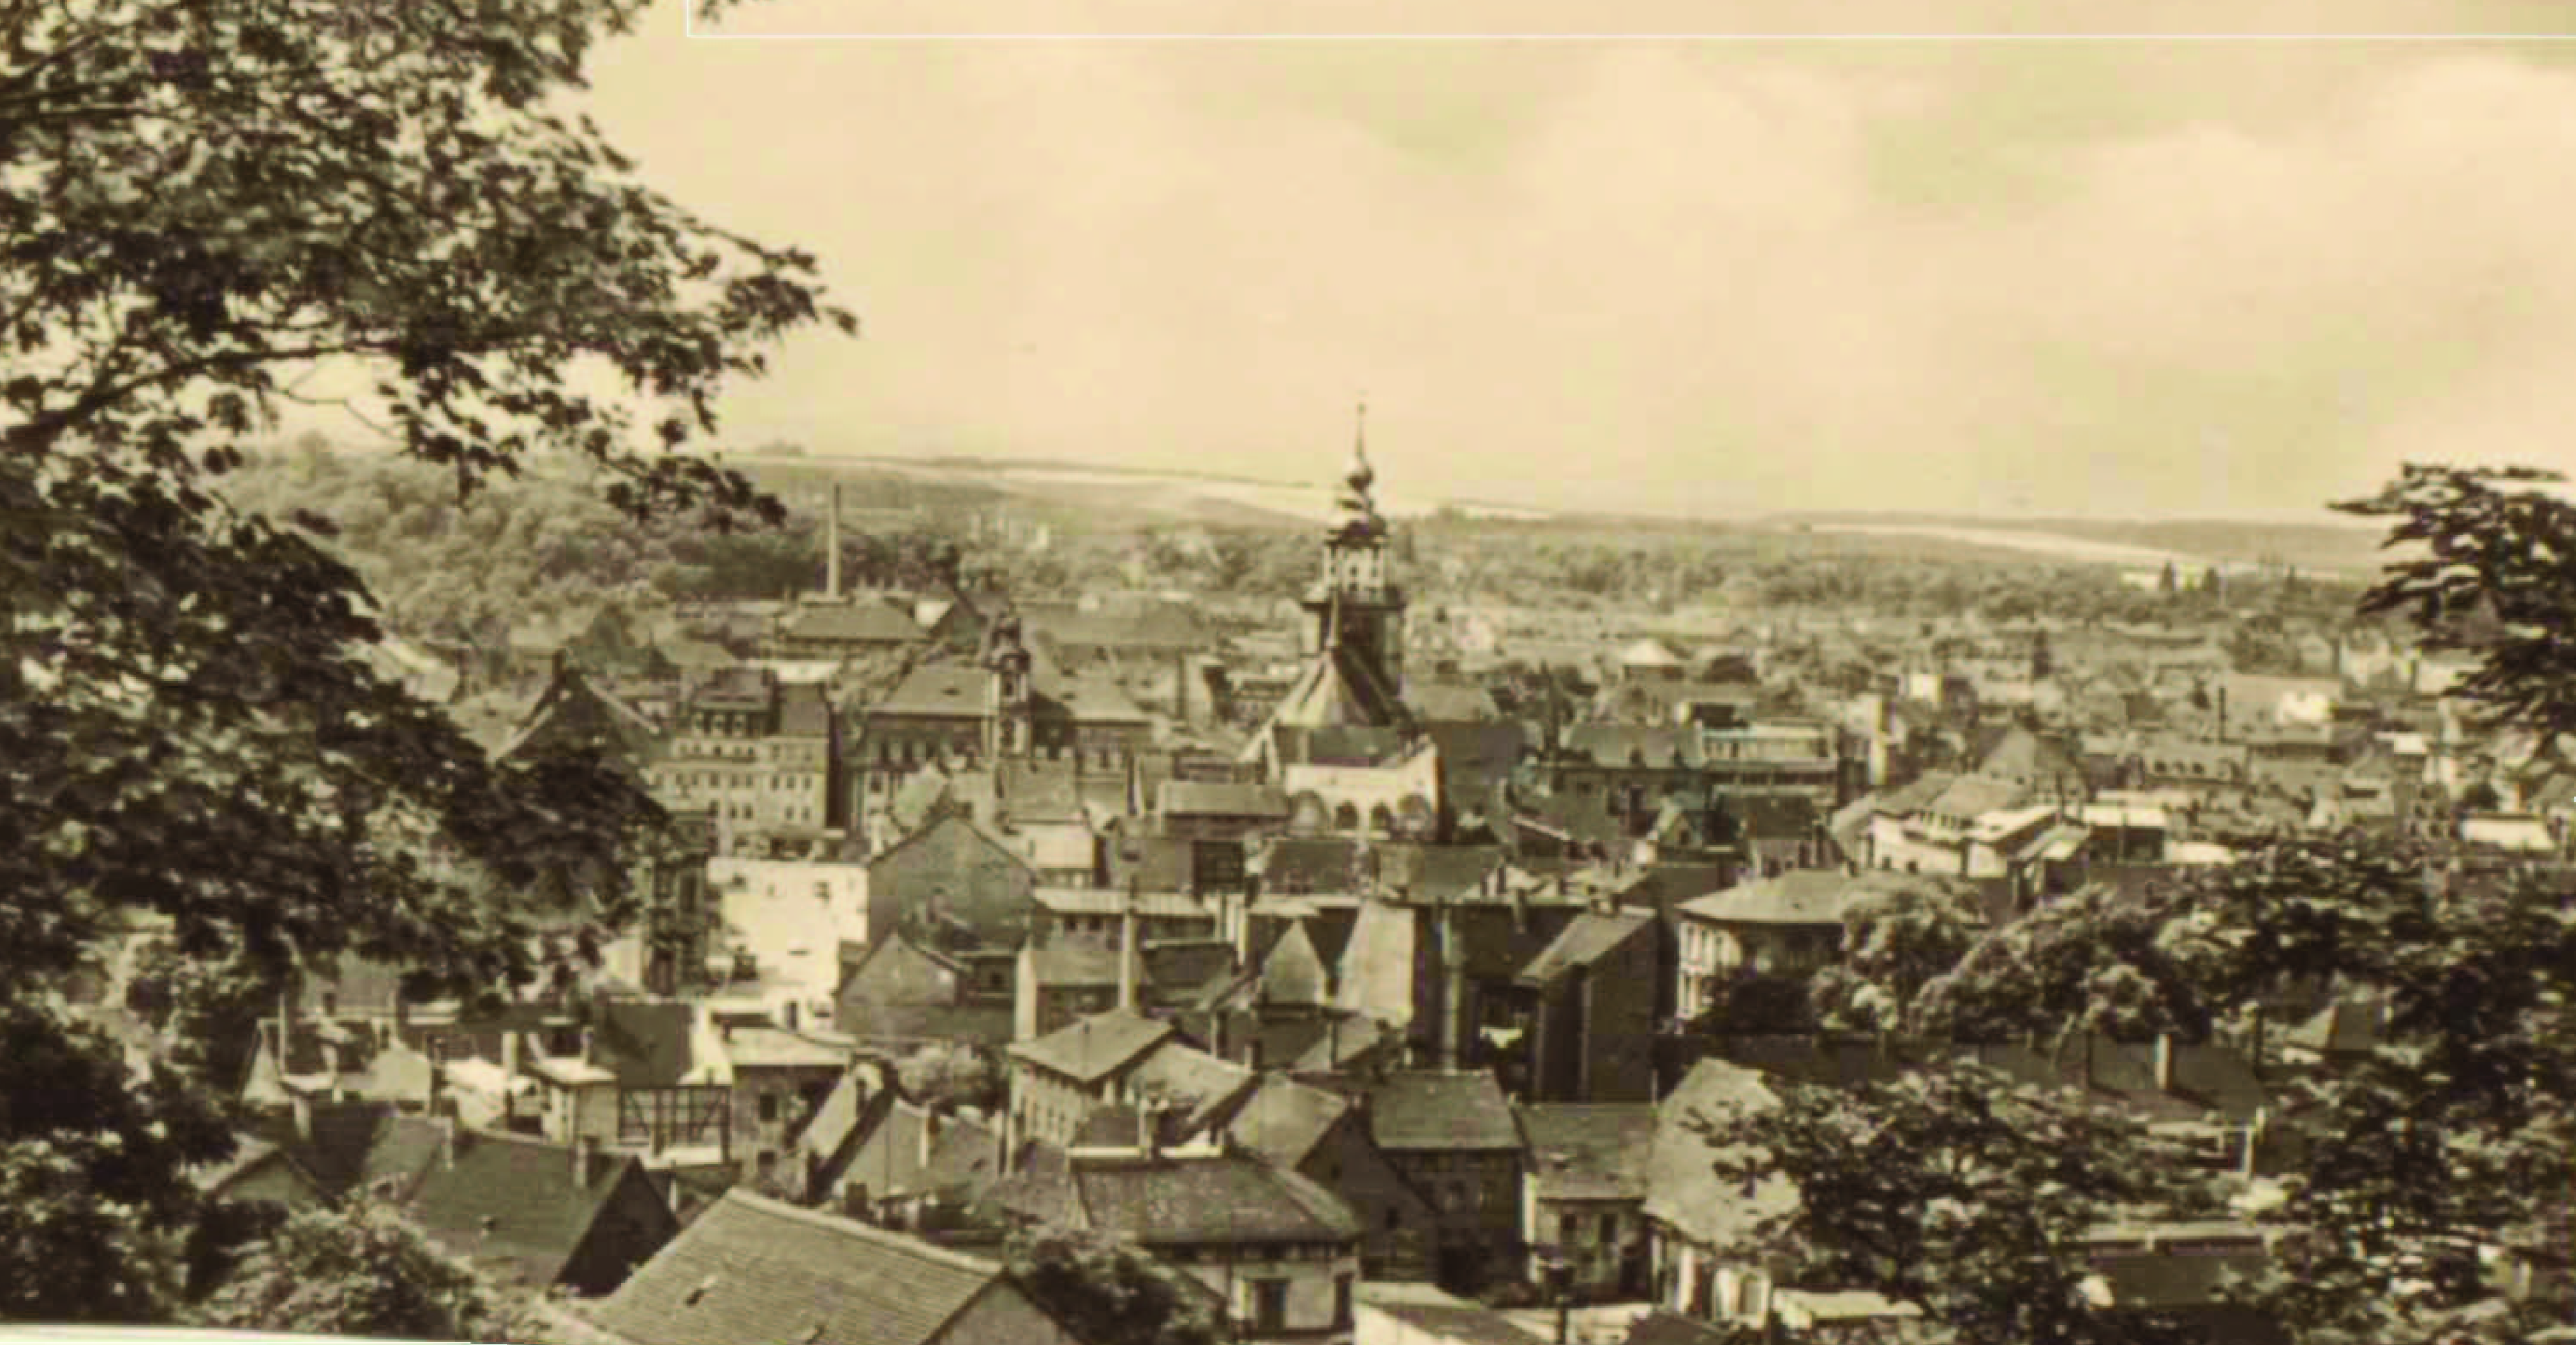
\includegraphics[width=\textwidth, height=\textheight, keepaspectratio]{192-a-mesto_weisenfels}
\caption{V městě Weisenfels u Lipska žijí Prusíci, potomci Josefy Prusíkové, rodačky ze Šípů}
\label{fig:192-a-město_weisenfels}
\end{figure}

             \begin{figure}
\centering
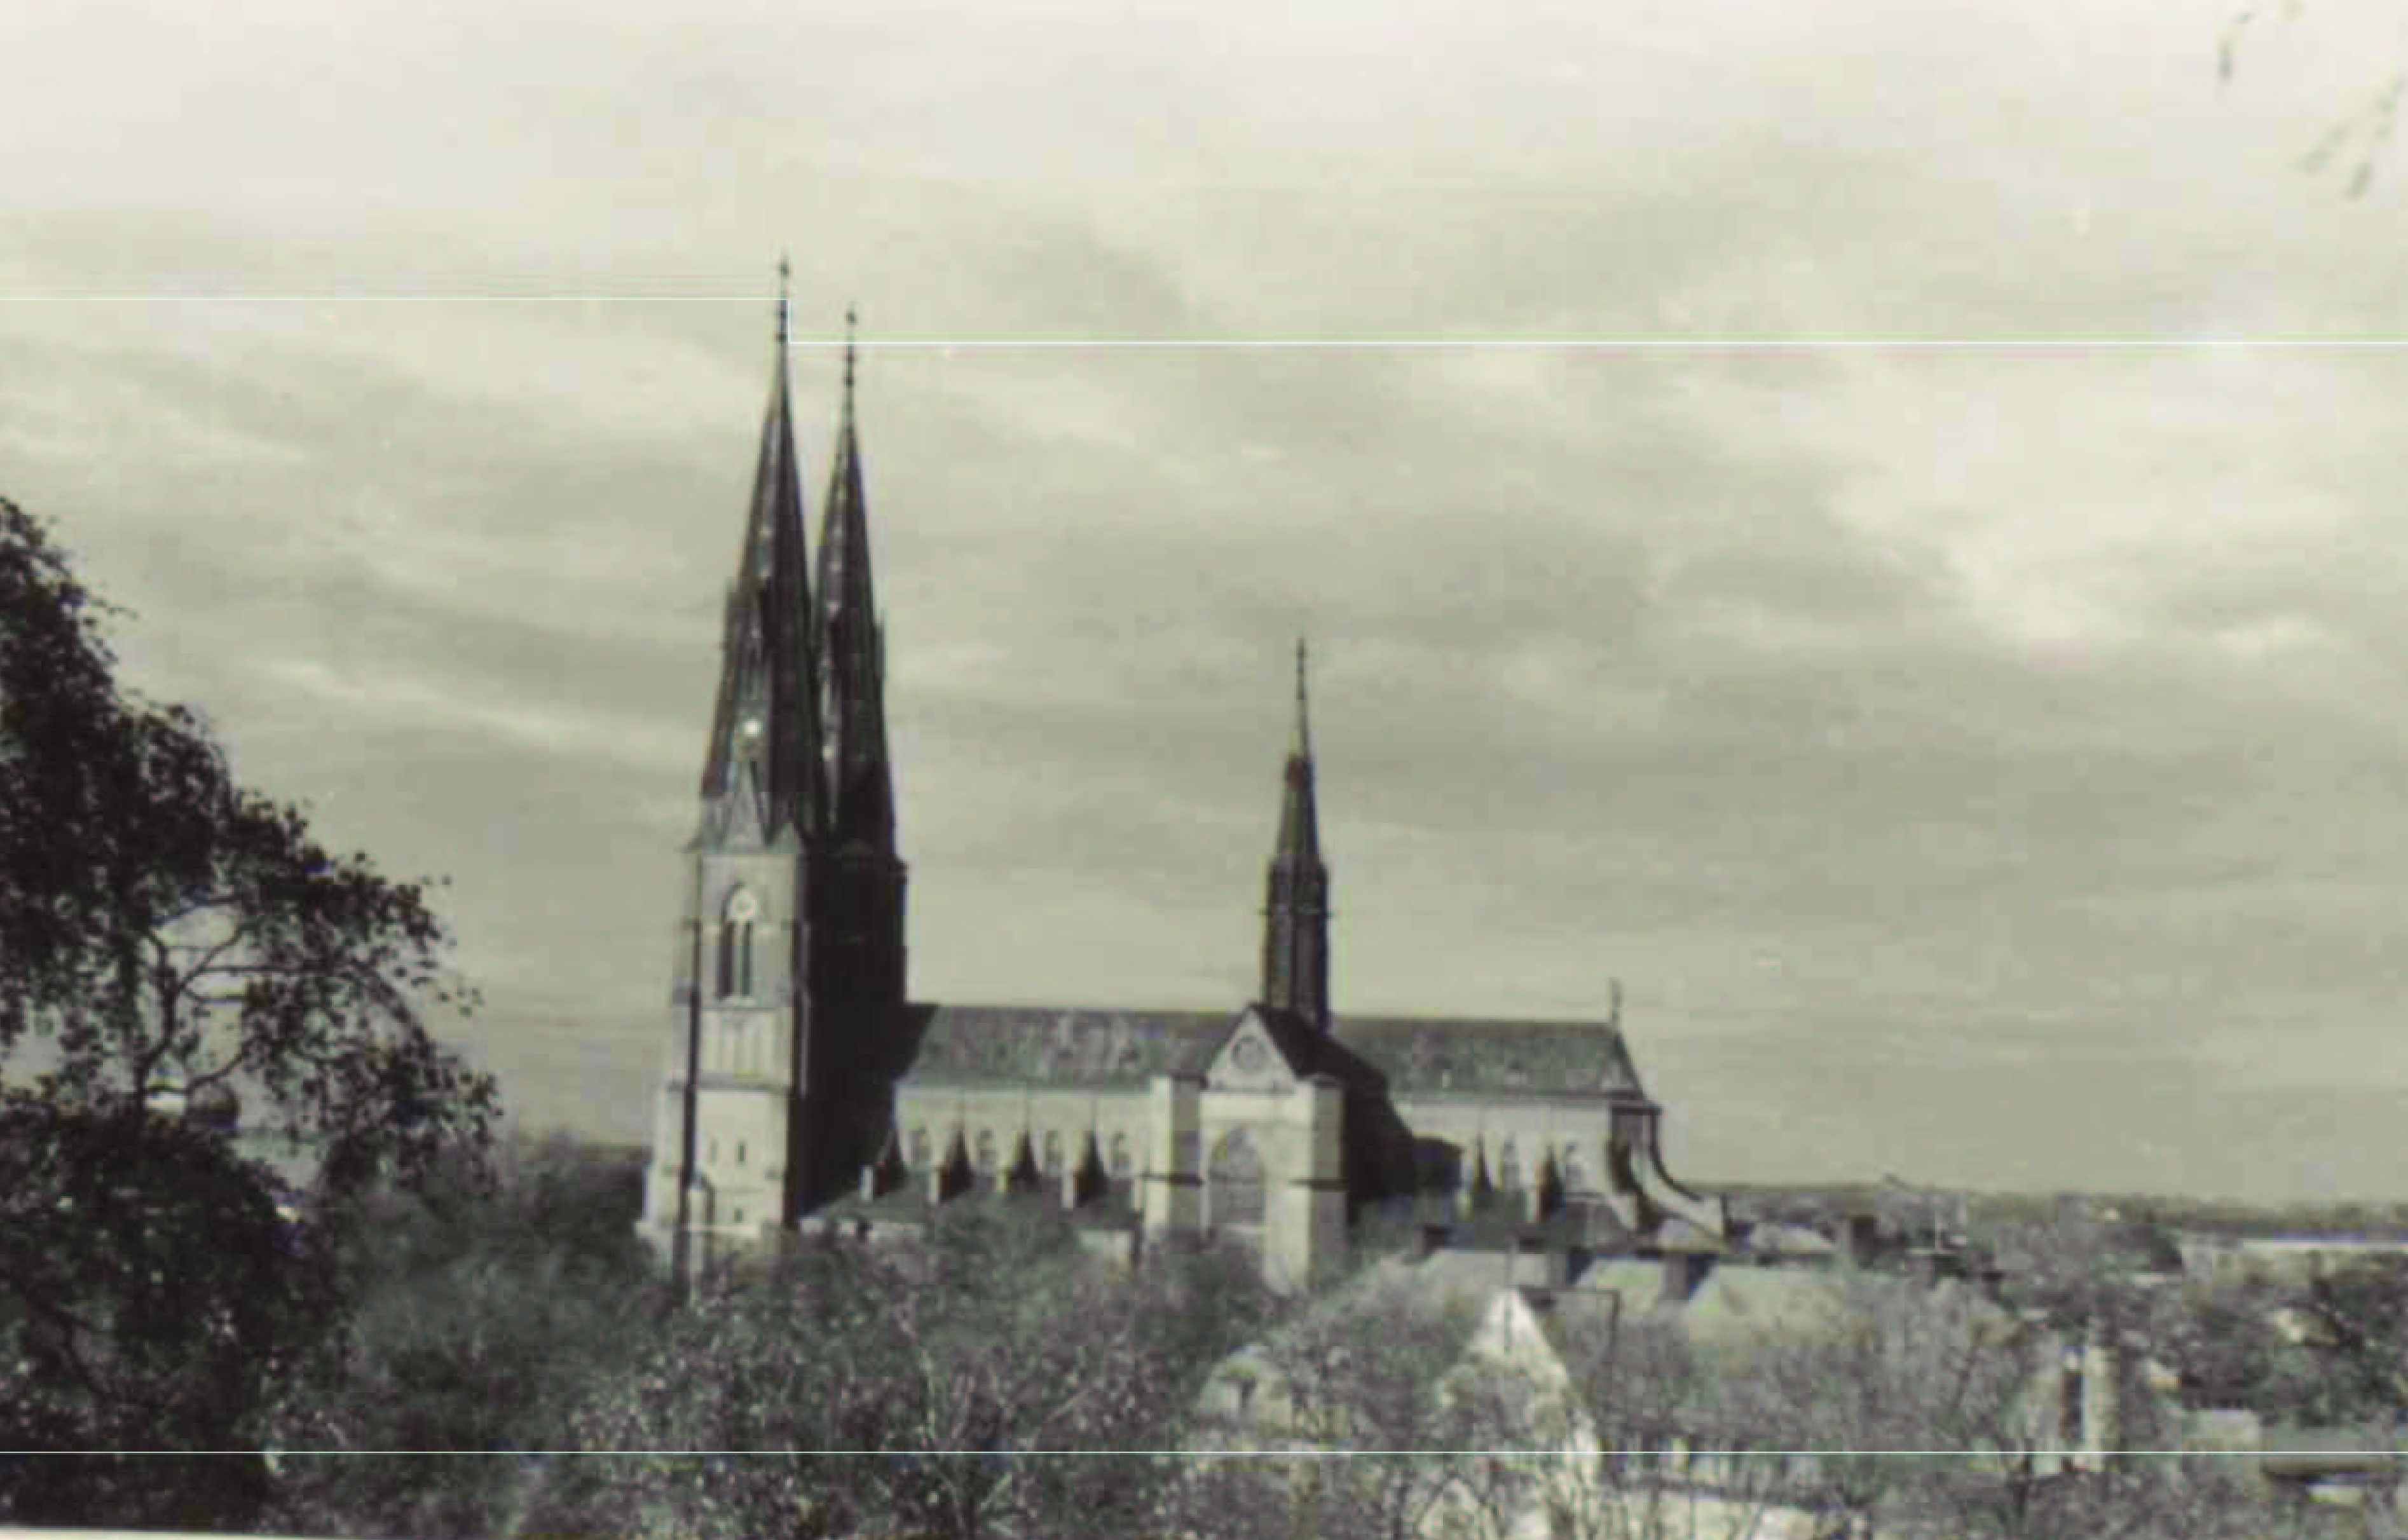
\includegraphics[width=\textwidth, height=\textheight, keepaspectratio]{192-b-katedrala_v_uppsale}
\caption{Pohled na katedrálu v Uppsale ve Švédsku, kde žije vnučka Josefy Prusíkové ze Šípů}
\label{fig:192-b-katedrala_v_uppsale}
\end{figure}

% str 168 @ 193
Josefa Gubová roz. Prusíková v Šípech měla ze všech svých sester nejtěžší život a při tom se dožila nej­delšího věku z nich. Příčinou jejího úmrtí byla uvede na stařecká sešlost. Ačkoliv to byla ryzí Češka, všechny její děti se poněmčily a mnozí potomci její jsou dnes již zase jiné národnosti. Nikdo z nich nežije v republi­ce.

První dítě Josefy Prusíkové byl nemanželský synek, který byl pokřtěn Edwin. Kdyby snad nebylo bývalo toho­to jejího nemanželského synka, který dostal po svobodné matce jméno Prusík, po Tomáši Prusíkovi ze Šípů by již nežili potomci s tímto jménem.

Edwin Prusík se narodil Josefě 25. 1. 1887 ve Veleticích u Žatce, kde sloužila. Otce nemanželského dítěte, i když nabídku dostala, si nechtěla vzít. Své dítě však brzy opustila a synek byl vychován u cizích lidí. Edwin Pru­sík byl dlouhá leta dělníkem ve šroubárně v Žatce. Bydlel ve Veleticích a jeden čas také v Novém Sedle u Žatce, později pak v Žatci až do roku 1946, kdy byl jako Němec odsunut. Edwin Prusík oženil se s Josefou Březinovou, roz. Horákovou 5. 2. 1889 v Zahrádce u Humpolce. S ní měl Edwin čtyři děti. Byli to dva syni a dvě dcery. První jeho manželka zemřela 28. 3. 1923 v Žatci. Edwin Prusík se pak podruhé oženil s Marií Gänzelovou nar. v Žatci 17. 4. 1883. Edwin Prusík byl odsunut do NDR a žije ještě dnes jako jeden z nejstarších Prusíků v městě Kőthen /Anhalt/, Geutzerstrasjse 40. Jeho druhá manželka tam zemřela 9. 4. 1959 a vdovec Edwin Prusík žije tam se svou dcerou Emmou.

Nejstarším dítětem Edwina Prusíka je syn Edwin. Narodil se 1. 10. 1908 v Novém Sedle u Žatce. Byl vyučen zámečníkem a po vystěhování z Československa žije dnes v městě Weissenfels (Saale), Georg Stöberstrasse 36. Pracuje nyní v hornictví. Jeho manželkou je Irmgard Fritschová nar. 8. 5. 1910 v Einsiedlu u Kamenice v Sasku. Edwin Prusík se svou manželkou Irmou má tři děti. Nejstarší je Edwin, který se narodil 3. 3. 1933 v Bohatících u Karl. Varů. Je ženatý, za manželku má Gerdu Schuhmannovou nar. 22. 6. 1934 v obci Tagewerben u města Weissenfelsu v NDR. Jejich adresa je tam: Weissenfelsstrasse 13. Edwin Prusík, toho jména již třetí v této rodině, pracuje v hornictví. Má dvě dcerky. Obě mají typická španělská jména. Carmen Prusíková se narodila 4. 9. 1959 a Manuela 13. 10. 1960. Jeho bratr Herbert Prusík narodil se 28. 7. 1939 v Karlo­vých Varech. Žije nyní také v městě Weissenfels, Katharinenstrasse 28. Herbert tam pracuje jako stavební mistr. Za manželku má Margrit (Markéta) roz. Hollsteinovou, 13. 1. 1940 ve Weissenfelsu. Mají synka Eyka nar. 27. 10. 1967 a v době, kdy píšeme a dokončujeme dějiny rodu Prusíků je Eyk Prusík nejmladším Prusíkem na světe.

Třetím dítětem Edwina Prusíka narozeného v roce 1928, je dcera Gudrun. Narodila se 9. 8. 1942 a dnes je provdaná Henková. Bydlí v Mecklenbursku v NDR v městečku Langenhanshagen (Kreis Ribnitz). Než se Gudrun vdala za Klause
% str 169 @ 194
Henka, měla nemanželského synka a ten se dnes jmenu­je Uwe Prusík. Narodil se 17. 1. 1961. Ze svého manžel­ství má dcerku Cornelii Henkovou nar. 11. 8. 1963.
Dalším dítětem Edwina Prusíka narozeného 1887, byla dcera Marie. Narodila se 25. 8. 1912 ve Veleticích u Žatce, provdala se za Václava Pöschla do Jindřichovic u Kraslic. Tam měli hostinec a její muž byl dosti exponován politicky. Marie Pöschlová roz. Prusíková žije nyní ve Fűrthu u Norimberka v NSR, Lessingstrase 7. Má tři děti. Její dcera narozená 27. 8. 1939 Inge, je provda­ná Kuchová a bydlí také ve Fűrthu. Má syna Berndta nar. v roce 1965. Syn Rudolf Pöschl narozený v listopadu 1943 je úředníkem ve Fűrthu. Dcera Margit nar. 22. 9. 1947 se provdala za amerického vojáka Dellbridge a v roce 1966 se jí narodil syn Michal. Žijí nyní v USA.

Třetím dítětem Edwina Prusíka, nemanželského syna Josefy, rodačky ze Šípů, byla dcera Emma. Narodila se 10. 4. 1914 ve Veleticích u Žatce. Brzy pak odešel jí otec do první světové války a vlastně všechny děti poznaly ho teprve po návratu z vojny. Emma je provdaná Kreutzmannová a bydlí v domku se svým starým otcem, vdovcem v Köthen. Je bezdětná.

Její druhý bratr je Rudolf Prusík. Narodil se 6. 12. 1917 ve Veleticích na Žatecku, vyučil se v potravinářském obchodě v Praze a snad on jediný z celé rodiny mluví ještě dobře česky. Je vedoucím potravinářského velkého podniku Supermarkt v Norimberku. Rudolf Prusík bydlí ve Fürthu v Bavorsku v NSR Horuschuchpromenade 34. Je­ho manželkou je Herta Reimová nar. 12. 8. 1922 v Třeskovicích u Žatce. Rudolf Prusík má dceru Karin nar. 2. 4. 1953 v Norimberku. Rudolf Prusík patří k těm členům ro­du našeho, i když je dnes již německé národnosti, kteří se rádi ke svému původu hlásí a členy rodu ve své původ­ní vlasti navštěvuje a u sebe v Německu rád vždy přivítá. Píšeme zde u jmen Prusík vždy čárku nad "i", ačkoliv v Německu se píší členové rodu jen s tečkou.

Když se Josefa Prusíková provdala za horníka Karla Gubu, žili spolu nejdříve v Třebušicích u Mostu a v Čachovicích u Března. Měli spolu pět dcer a jednoho syna. Nejstarší dcerou byla Emilie. Narodila se 8. 12. 1897 v Čachovicích. Provdala se v roce 1927 za mechanika Ladislava Villányiho maďarského původu. Do roku 1938 žili spolu v Československu. Pak se přestěhovali do Budapešti, kde Emilie Gubová provdaná Villányiová zemřela po pohnutých událostech maďarských 21. 11. 1956 v Budapešti. Emilie měla dvě dcery. Starší byla Emilie, která se narodila 31. 12. 1929 v Rybářích u Karlových Varů. Studovala na universitě v Budapešti geologii. Ještě v Maďarsku provdala se za che­mika Jiřího Fuchse a od roku 1956 žijí spolu ve Švédsku. Bydlí ve starobylém universitním městě Uppsale, Tunagaten 32-a. Její manžel přednáší na vysoké škole v Uptuně u Uppsaly. Emilie Fuchsová pokračovala ve studiu geologie
% str 170 @ 195
i ve Švédsku, ale když se jí narodily děti, zůstala doma. Má syna Roberta Fuchse nar. 27. 1. 1961 a dceru Annu nar. 6. 9. 1963. Její sestra Zelma narodila se 29. 1. 1931 v Chomutově. Žila pak také s rodiči v Bu­dapešti a se svým mužem Molnarem opustila v roce 1956 Maďarsko. Je dnes doktorkou pathologie a pracuje a přednáší na universitě v Chicagu v USA. Její muž je docentem. Bydlí v Chicagu, 60615 (Illinois) 5778, S. Everett. Dr. Zelma Molnarová má dvě děti. Syna Petra nar. 5. 12. 1962 a dcerku Reku nar. 7. 3. 1965.

Druhou dcerou Josefy Gubové, roz. Prusíkové byla Marie. Narodila se 10. 6. 1899 v Čachovicích. Byla provda­ná Malinová. Její muž byl horníkem. Po odsunu z republi­ky v roce 1946 žila v městě Güsen u Magdeburgu v NDR. Marie Malinová zemřela tam náhle 10. 12. 1967. Měla dva syny. Antonín Malina nar. 24. 12. 1919 bydlí v místě Parey-Elbe, Neuer Weg 4, Kreis Genthin v NDR. Pracuje tam v průmyslu. Má jednoho syna Klause, nar. 16. 2. 1954. Bratr Antonínův, Adolf Malina narodil se 5. 3. 1922. Žije a pracuje v Poruří v NSR. Bydlí v městě Hattingen, Berlinerstrasse 2. Má synka Františka Mali­nu nar. 7. 2. 1961. Adolf malina zemřel 18. listopadu 1968 na rakovinu.

Další dcerou Josefy Gubové byla Irma. Narodila se 19. 6. 1901 v Čachovicích u Chomutova. Byla provdaná za Jindřicha Kőrnera, rodáka z Dubí. Od roku 1920 žili v Chomutově, u ní žila také její maminka, roz. Prusíková, která prý až do smrti se nikdy nenaučila pořádně německy. Děti její se bohužel odnárodnily. Irma Kőrnerová měla pět dětí. Její dcera Herta nar. 8. 8. 1926 byle provdaná Hankeová, ale zůstala bezdětná. Zemřela v městě Stephershausenu kraj Meiningen v NDR, v roce 1953. Druhé dítě Irmy byl Eduard Kőrner. Narodil se 16. 2. 1928 a po různém bloudění dostal se až do Australie. Žije a pracuje tam dnes v Sydney, Gremorne 67, Wyongr Road.

Pak se narodila Irmě Kőrnerové dvojčata. Je to Alma Kőrnerová nar. 23. 7. 1932 je zdravotní sestrou a zůstala svo­bodná. Bydlí v městě Karl Marx Stadt Abeestrasse 1, NDR. Další dvojče je její sestra Elfrieda. Byla dlouho balet­kou. Dnes je provdaná Süssengutrová a bydlí v Greifswaldu J. S. Bach Strasse, č. 41 v NDR na břehu Baltu. Elfrieda má slušnou kupu dětí. Je jich pět. Dcerka Andrea se narodila 1. 4. 1952, Claudia 11. 1. 1955, syn Thomas Süssengut nar. 8. 2. 1957 a zase pak dcerky, Gabri­ela nar. 23. 7. 1959 a Anna 9. 11. 1954.

Nejmladším dítětem Irmy Kőrnerové byla dcera Waltraud. Narodila se 8. 9. 1942. Byla učitelkou v mateřské školce, provdala se za Mohameda Abdallu, který studoval na universitě tropické zemědělství. Pochází ze Sudanu v Africe. Manželé zatím žijí spolu v Lipsku, Karl Liebknechtstrasse 17. Pravděpodobně však přesídlí spolu do Afriky. Od 30. 7. 1967 mají synka jménem Usama. Irma Kőrnerová roz. Gubová zemřela 1. 12. 1963 v městě Gőssnitz v NDR.

% str 171 @ 196
Syn Josefy Gubové roz. Prusíkové, Karel byl pojmenován po otci. Narodil se 14. 6. 1900 v Čachovicích u Chomutova. Byl horníkem jako jeho otec a zemřel 29. 9. 1954 v městě Schlema v Rudohoří v NDR. Měl čtyři děti. Jeho syn Antonín Guba nar. 25. 2. 1931 v Hořanech u Mostu žije také v obci Schlema. Bližší jeho adresa je 9408 - Schlema I. /Erzgebirge am Flossgraben 3, DDR. Antonín Guba pracuje také v hornictví. Má dvě děti. Jeho dcera Waltraud je narozena 19. 12. 1949 a syn Dietmar Guba 19. 2. 1953.  Dalším dítětem Karla Guby je dcera Ursula. Narodila se 18. 7. 1939 v Mostě. Dnes žije také v obci Schlema. Je svobodná. Syn Karel Guba nar. 25. 5. 1942 zemřel svobodný v l8-ti letech 11. 1. 1960. Posledním dítětem Karla Guby byl syn Gerhard. Narodil se 4. 2. 1945 a žije s matkou ta­ké ve městě Schlema v NDR.

Dalším dítětem Josefy Gubové, roz. Prusíkové byla dcera Anna. Narodila se v roce 1903  a byla provdaná Salzerová v Hořanech u Mostu. Měla dva syny. Rudolfa Salzera nar. 1. 1. 1925 a Františka nar. 21. 12. 1923. Oba padli jako vojáci německé armády na ruské frontě.

Poslední dítě Josefy Gubové byla Emma. Narodila se l8. 10. 1906 ve Slatinicích u Mostu. Provdala se za Viléma Enzmanna a z Chomutova byla odsunuta roku 1946. Nyní žije jako vdova v Bambergu, Marienplatz 2 v NDR. Je bezdětná a navštěvuje hojně všechny své příbuzné v NDR i NSR. Také má o nich, ať žijí kdekoliv ve světě, ten nejlepší přehled.

Tím jsme popsali život Josefy Prusíkové ze Šípů a osudy jejích potomků. Jsou jistě pestré a dnes jsou roztroušeni v obou německých státech, ve Švédsku, USA i Austrálii. V našem rodě není takových rodin mnoho.

To byly tedy v krátkosti příběhy a život celé rodiny Tomáše Prusíka, který se narodil v dobách roboty v Sedlici, pak se usadil v Šípech u Čisté a tam v nece­lých svých čtyřiceti letech zemřel. Měl jen dcery, které dospěly, ale přesto, po té nejmladší Josefě, žiji opět dnes lidé s jménem Prusík i když již ne v naší vlasti, ale v cizině.
Tomáš Prusík zanechal po sobě 157 potomků, z toho již 23 mrtvých v době, kdy Končíme dějiny našeho rodu.

% str 171+1 @ 197
\begin{figure}
\centering
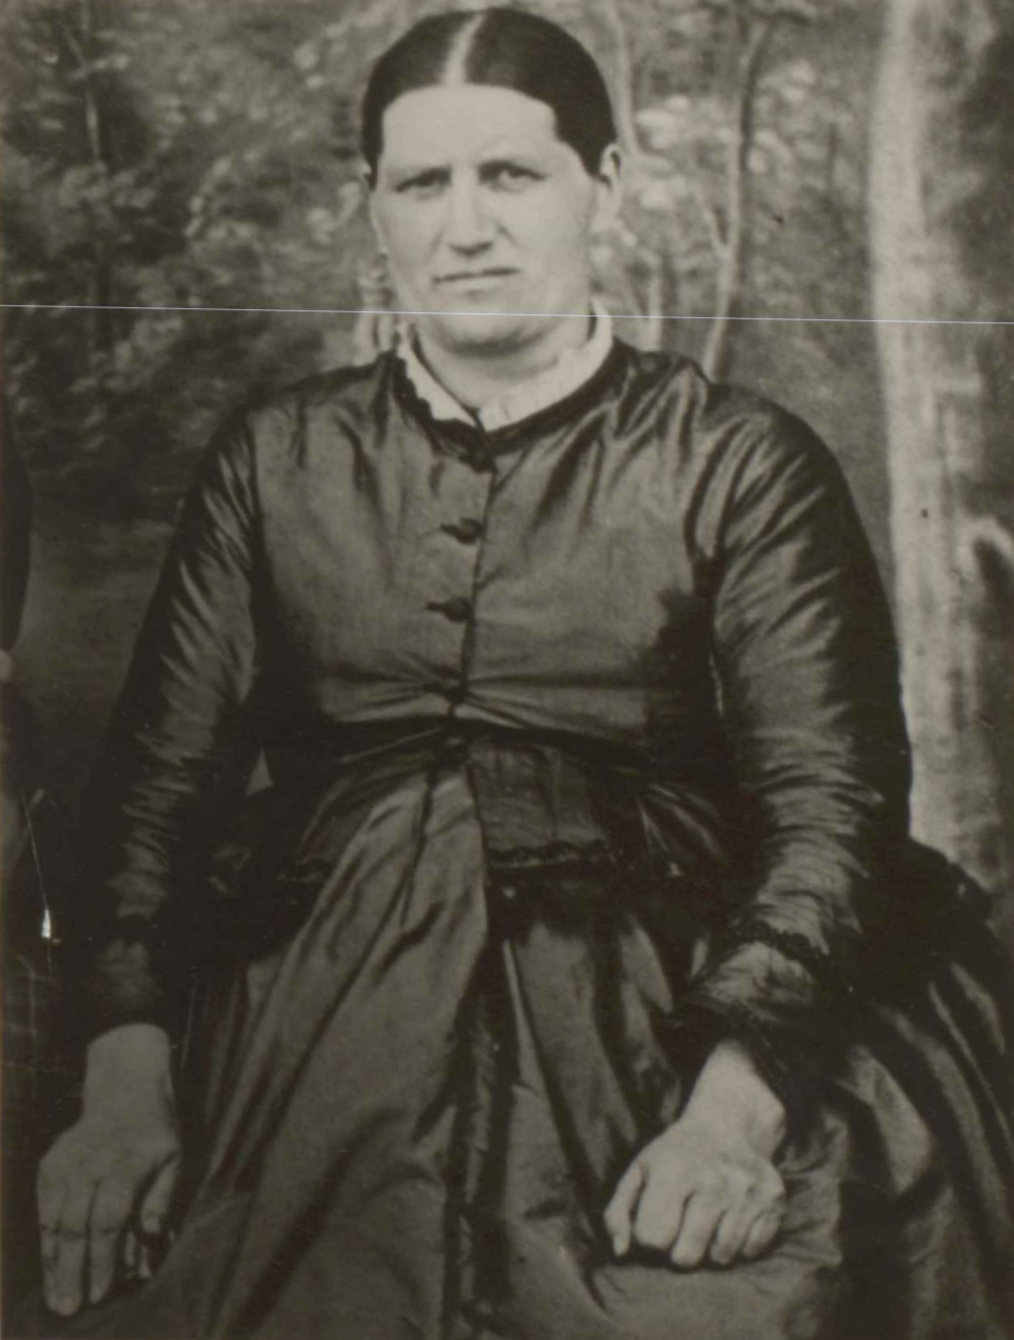
\includegraphics[width=\textwidth, height=\textheight, keepaspectratio]{197-marie_prusikova_1845}
\caption{Marie Prusíková (1845 – 1925), narozená v gruntě v Sedlci č. 4. Jejím provdáním za Vojtěcha Čecha do Chrašťovic v roce 1867 mizí jméno Prusíků ze Sedlce. Prokazatelně tam byl rod 352 let}
\label{fig:197-marie_prusikova_1845}
\end{figure}


% str 172 @ 198
\section{Odnož Sedlec - větve Sedlec}

Potomci Františka Prusíka ze Sedlce, který byl posledním hospodářem v tomto gruntě, kde stála první kolébka rodu.

1825 - 1846

Posledním synem Václava Prusíka, rychtáře v Sedlici byl František. Narodil se v gruntě č. 4, jak byl v ro­ce 1805 přečíslován z dosavadního čísla 9. František Prusík narodil se 6. 7. 1825. V roce 1844 oženil se s Bar­borou Fronkovou, která se narodila 17. 6. 1827 v Chrašťovicích. V roce 1845 převzal po otci grunt. František Prusík měl se svou ženou Barborou jednu dceru Marii nar. 8. 12.1845. Ta však svého otce ani nepoznala, neboť ten zemřel ve věku 21 let na zápal plic 14. 6. 1846. To byl poslední Prusík po meči na gruntě, kde již v roce 1515 za panování krále Vladislava Jagellonského hospodařil náš rod. Mladá, devatenáctiletá vdova vdala se v roce 1849, 12. února za Františka Pittnera z Vysoké Libyně. Ten však za sedm let zemřel a v roce 1857 se Barbora provdala po třetí za Antonína Urbana.

Jak nám vypravoval Václav Urban, který až do roku 1952 hospodařil na gruntě "u Prusíků" v Sedlci, říkalo se zde vždy "na staré rychtě". Ještě v roce 1962 stála u statku stará stodola, vystavěná někdy po třicetileté válce. Tehdy také ještě existovaly světnice podruhů, ovšem z části rozbourané. I tato dřevená stavba byla asi 250 let stará.

Sirotek po Františkovi Prusíkovi, Marie žila pak doma se svou matkou znovu provdanou a když nabyla v roce 1867 plnoletosti bylo jí vyplaceno 3000.- zlatých a ona se vdala za sedláka Vojtěcha Čecha v Chrašťovicích. To se stalo 12. 2. 1867. Polovina usedlosti, která do té doby byla zapsána na její jméno, byla odepsána a tím dnem mizí na věky jméno Prusík nebo Prusíková z gruntovních a pozemkových knih u tohoto statku, kde 352 let žil pro­kazatelné náš rod. Možná, že tam existoval již dříve za krále Jiřího z Poděbrad a před ním, ale o tom nejsou doklady. Je tedy Marie Prusíková provdaná Čechová takovou legendární osobností rodu, jako je první náš známý předek Vojtěch Prusík, narozený v téže usedlosti 1515. Barbora Urbanová, kdysi provdaná Prusíková, zemřela v Kralovicích u svých příbuzných z dalšího manželství na souchotiny 9. srpna 1898.

Marie Čechová. roz. Prusíková, jediné dítě Františka Prusíka ze Sedlce, měla řadu dětí. Dospělo jich osm. Byli to čtyři synové a čtyři dcery. Všechny její děti narodily se v Chrašťovicích. Její muž, který býval starostou Chrašťovic, Vojtěch Čech, byl velkým dobrá­kem, hodně půjčoval lidem a ti mu často dluhy nespláce­li. Hospodářství jejich se tak dostalo do peněžní tísně, museli je prodat a z toho co zbylo, zakoupila se usedlost v Rokycanech. Ke konci života Marie Čechová žila jako vdova u své dcery Anny provdané Stupkové v Praze a zde, milována všemi svými dětmi, dokončila svůj život 1. 11. 1925.

% str 173 @ 199
Marie Čechová, roz. Prusíková ze Sedlice je pohřbena na Olšanských hřbitovech v Praze.

Nejstarším dítětem Marie Čechové byl syn Josef. Narodil se 9. 11. 1874 v Chrašťovicích. Celý svůj život věnoval se restauračnímu podnikání. Byl také vyučený ku­chař, rozuměl i hotelnictví, býval nájemcem Variété v Praze-Karlíně, míval velký hotel v Gradu v Itálii a ve svém oboru dosáhl mnoho úspěchů, a ovšem i mnoho neúspěchů, jak to nese risiko podnikání. Josef Čech zemřel náhle v Praze, před štědrým dnem 23. 12. 1932. Měl dvě děti. Jeho dcera Marie narodila se 24. 6. 1900, vystudovala Obchodní akademii a Konservatoř v Praze, pak se provdala za lékaře Jana Pihlara, Slovince z Mariboru, který po první světové válce studoval v Praze a zdokonaloval se na klinikách u prof. Pelnáře a prof. Prusíka. Marie se pak s ním odstěhovala do Jugoslávie, kde bydlí v Mariboru, Prešernova 2. Její muž Dr. Janko Pihlar byl tam primářem v nemocnici a ještě dnes provozuje soukromou ordinaci. Marie Pihlarová, roz. Čechová má čtyři děti. Její syn Dr. Janko Pihlar nar. 31. 1. 1931 v Mariboru, stal se také lékařem jako otec a bydlí tam v Kmetíjské ulici 3a. Dr. Janko Pihlar má dcerku Soňu nar. 25. 1. 1960. Další dítě Ma­rie Pihlarové, je dcera Markéta, které říkají v rodině Lily. Narodila se 6. 1. 1933 a je provdánu za inž. Hidassi maďarského původu. Žijí v Butzbachu, Pohlgőnserstrasse 5. Toto město leží v Hessensku v NSR. Lily Hidassiová má dvě děti. Dcerku Claudii nar. 23. 6. 1965 a synka Petra nar. 11. 10. 1966. Druhý syn Marie Pihlarové je Josef. Narodil se tentýž rok jako jeho sestra Lily, ovšem až ke konci 26. 12. 1933. Je veterinářem a doktorem v tomto oboru. Hledal lepší uplatnění svých znalostí a žije dnes v USA v městě Omaha v Nebrasce, Apartment 20,-4750 Lafayette Avenue. Dr. Josef Pihlar je svobodný. Čtvrtým dítětem Marie Pihlarové je dcera Marieta. Narodila se 17. 10. 1944 v Mariboru a provdala se za úředníka Klisa, ro­dáka z Lopudu u Dubrovníka. Mají dcerku Irenu nar. 12. 4. 1965.

Marie Pihlarová roz. Čechová je neobyčejně inteligentní žena a přesto, že téměř 45 let žije v Jugoslávii, mluví i píše výborně Česky.

Druhým dítětem Josefa Čecha byl syn Bohumil. Narodil se 22. 12. 1902, studoval technický obor v Německu, aby tam rozšířil svůj obzor, míval svůj elektrotechnický obchod, ale i jemu se po květnu 1945 mnohé velké plány zhatily. Je ženatý, ale bezdětný a žije dosuď v Sedlčanech, Gottwaldova 43. Nyní bydlí v Praze 10, U hranic 5.

Druhým dítětem Marie Čechové roz. Prusíkové byla dcera Růžena. Narodila se 12. 5. 1879 a provdala se za cukráře Trykara ve Spáleném Poříčí. Její manželství bylo bezdětné. Ve Spáleném Poříčí Růžena Trykarová zemřela dne 10. 10. 1938.

% str 173+1 @ 200
\begin{figure}
\centering
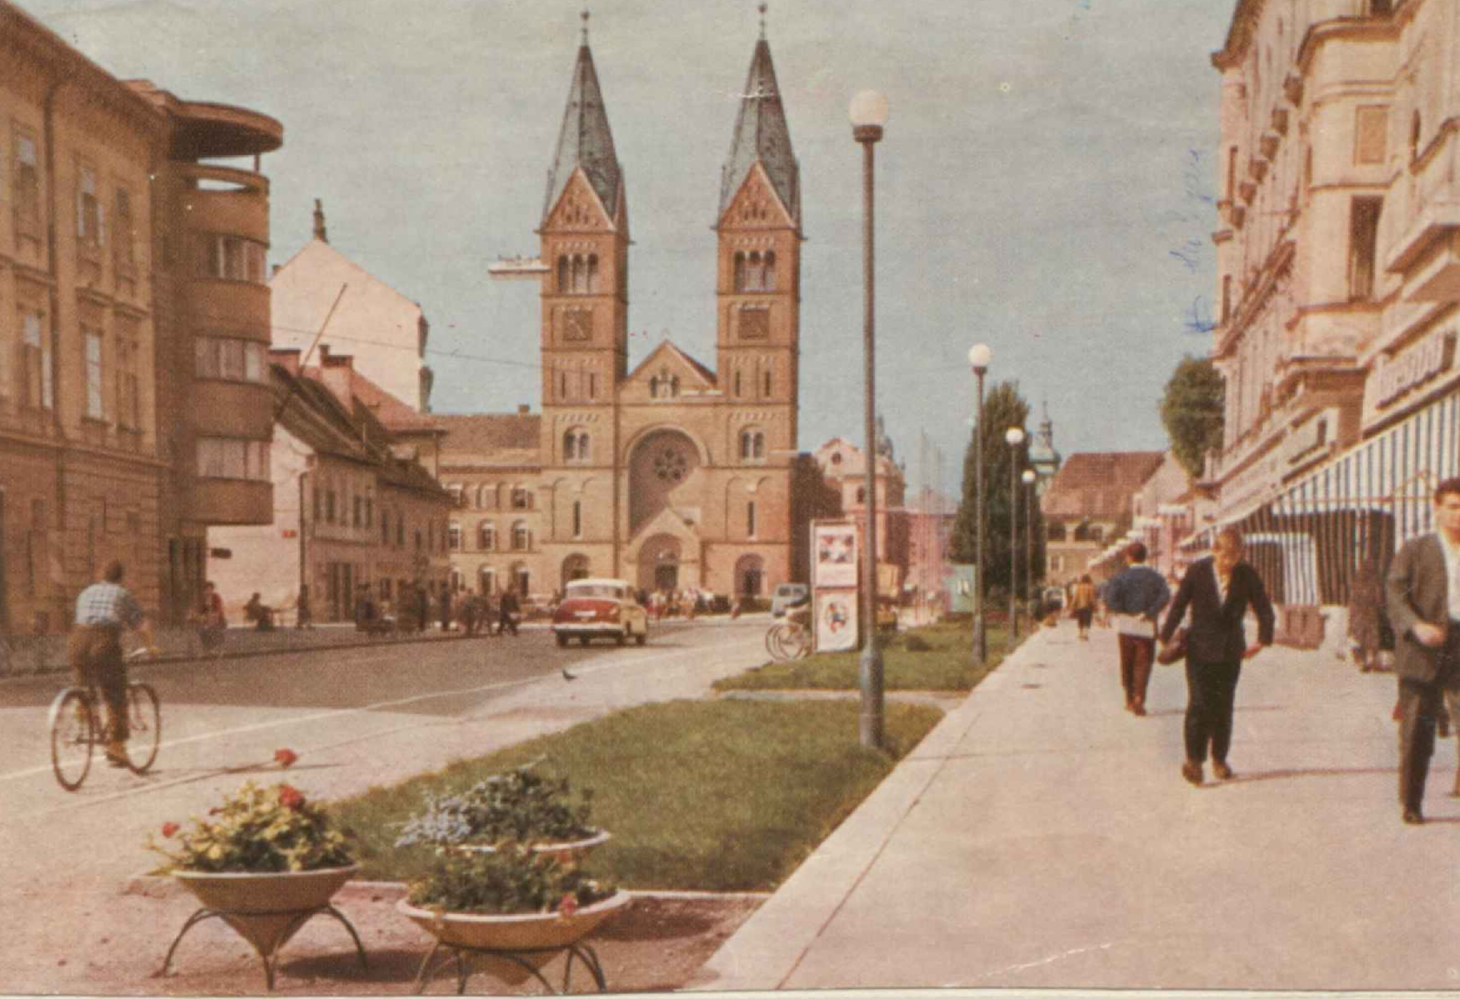
\includegraphics[width=\textwidth, height=\textheight, keepaspectratio]{200-a-maribor}
\caption{Maribor v Jugoslávii, kde je usedlá Marie Pihlarová, vnučka Marie Prusíkové provdané Čechové, rodačky ze Sedlce}
\label{fig:200-a-maribor}
\end{figure}

\begin{figure}
\centering
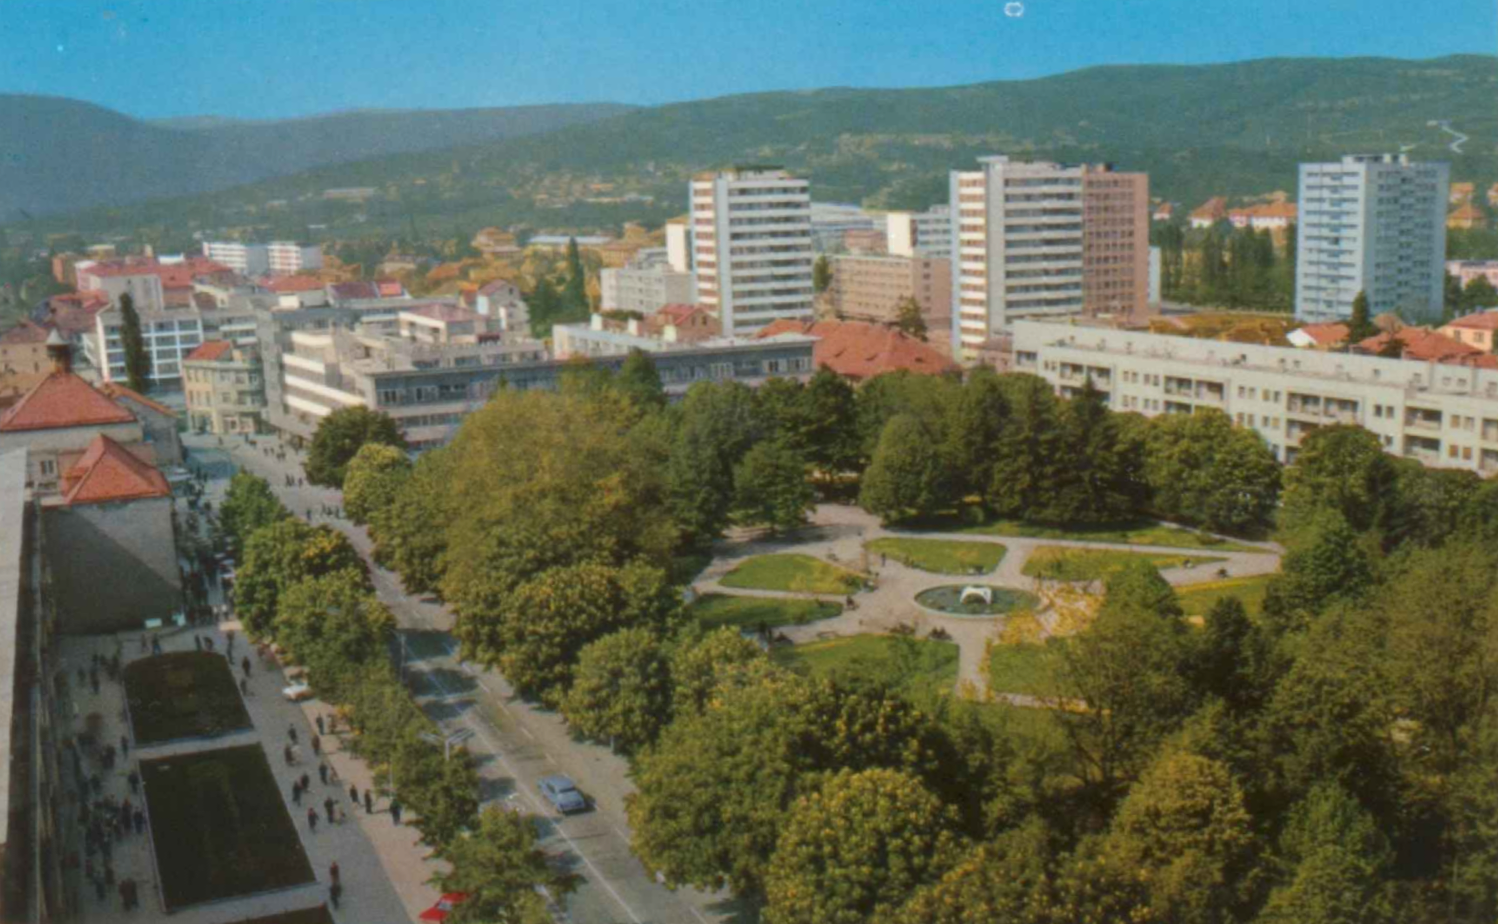
\includegraphics[width=\textwidth, height=\textheight, keepaspectratio]{200-b-banja_luka}
\caption{Pohled na Banja Luku v Jugoslávii, kde žije Otylie Jedličková, potomek Marie Čechové, rozené Prusíkové}
\label{fig:200-b-banja_luka}
\end{figure}


% str 174 @ 201
Třetím dítětem Marie Prusíkové provdané Čechové byla Anna. Narodila se 19. 7. 1881 a provdala se za majitele řeznictví a uzenářství Norberta Stupku, rodáka z Rokycanska. Měli velký podnik výrobní v Praze na Vinohradech ve Slezské ulici. Anna Stupková zemřela poměrné mladá 11. 8. 1929 v Praze, jen čtyři roky za svou mat­kou, které dosloužila k smrti. Anna Stupková měla tři syny a jednu dceru. Nejstarší byl Oldřich nar. 18. 2. 1904 a zůstal doma v řeznickém podniku otcově v Praze na Vinohradech. I on v květnu 1945 dopadl špatně, vzali mu nejen dům a podnik, ale ještě jej poslali do jáchymov­ských dolů. To mu také podstatně zkrátilo život. Zemřel 7. 1. 1961 v Petrově u Davle, kam byla rodina násilné z Prahy vystěhována. Oldřich Stupka měl dva syny. Jeho syn Norbert narodil se 9. 6. 1932 a pracuje v Geologic­kém průzkumu, bydlí v Praze - Žižkově, Na vrcholu 2583. Má dcerku Ingrid Stupkovou narozenou 18. 9. 1964. Druhý syn Pavel Stupka narodil se 9. 4. 1938 a pracuje také ja­ko jeho bratr v Geologickém průzkumu. Za ženu má lékař­ku, ale děti zatím nemají. Bydlí v Praze Dejvicích, Ždanovova 65.

Druhý syn Anny Stupkové je Vladimír. Narodil se 30. 3. 1905, býval úředníkem ve Státní bance. Toto místo pro svůj původ musel opustit a pak se stal instalatérem. Nyní žije na odpočinku v Praze-Bráníku ul. Ke Krči 15-806. Je ženatý ale bezdětný.

Dalším dítětem Anny Stupkové je dcera Božena. Narodila se 22. 12. 1906. Nejdříve byla provdaná za inženýra Hoška, podruhé za soudce Dr. Chaloupku v Teplicích. I ona doplácela na svůj "špatný“ původ. Nezbylo jí také nic z majetku po rodičích. Bydlí v Praze-Žižkově, Žerotínova 42. Byla úřednicí ve výsadní společnosti Motokov. Z prvního manželství má dceru Zorku provdanou Rysovou, která je však rozvedena. Narodila se 7. 7. 1932 a bydlí v Praze-Malešicích, Počernická 512. Děti nemá. Druhé dítě Boženy Chaloupkové, roz. Stupkové je z druhého manželství syn Karel. Narodil se 4. 9. 1937 a bydlí v Praze Žižkově, Žerotínova 39, blízko své matky. Pracuje v zemědělském oboru, je ženatý ale dosud bezdětný. Poslední dítě Anny Stupkové je syn Norbert. Narodil se 4. 8. 1908 v Praze. Původně měl hospodařit, ale i s ním osud jinak zatočil. Stal se údržbářem. Žil dosti dlouho v Plzni, kde měl vilku, dnes bydli v Ostravě, Spanieleva ul. 925. Norbert Stupka má dva syny. Jeho syn Jaroslav naroz. 25. 9. 1937 je chemikem a byd1í v Plzni, Kolerovská 428. Má dvě dcery: Olgu nar. 26. 4. 1968 a Renatu nar. 9. 7. 1963. Druhý syn Nor­berta Stupky Miloslav, nar. 10. 8. 1943 je elektrotechni­kem a žije v Karlových Varech — Tuhnicich, Krymská 30-D. Má synka Martina Stupku nar. 24. 12. 1963.

Abychom byli opravdu přesní, prvním dítětem Marie Prusíkové, provdané Čechové byla dcera Terezie a třetím jejím dítětem Marie. Terezie Čechová narodila se 3. 10. 1872 v Chrašťovicích. V pozdějším věku provdala se za inženýra Kašpárka, ale
% str 175 @ 202
brzy ovdověla. Pomáhala pak v domácnosti své sestry Anny Stupkové v Praze a smrt ji zastihla v Rokycanech, kde právě dlela u své sestry Marie. Zemřela 17. 4. 1945 a její pohřeb se konal za leteckého náletu.

Marie, sestra Terezie a Růženy, narodila se dne 13. 3. 1877 v Chrašťovicích. Byla provdána za řezníka Mejstříka v Rokycanech, člověka poměrně hrubého. Měla dvě dcery. Marii nar. 7. 7. 1899, která zůstala svobodná a pomáhala také v domácnosti své tety, Stupkové v Praze. Zemřela tragicky v roce 1924. Uhořela, když zapalovala v kamnech pomocí hořlaviny. Druhá dcera  byla Otylie nar. 9. 6. 1901. Jako její sestřenice Marie Čechová, provdaná Pihlarová v Jugoslávii, i ona vzala si Jugoslávce inženýra Jedličku a žije dnes v Banja Luce, ul. V. Masleše 21/II v Bosně. Otylie Jedličková je bezdětná. Druhý syn Marie Prusíkové, provdané Čechové, byl Vojtěch. Narodil se 10.  5. 1883. Uvažovalo se o něm, že převezme rodný grunt v Chrašťovicích, který měl 200 strychů (57,5 hektarů). Vojtěch Čech zemřel však již 24. 3. 1893 a grunt byl pak v roce 1912 prodán.

Další syn byl Bohumil Čech. Narodil se 15. 6. 1885. Byl finančním úředníkem a dosti dlouho působil na Slovensku. Matka pro něj, jak vždy prohlašoval, byla světicí. Před svou smrtí nebyla vůbec nemocná a i když dožila se pěkného věku 80 let nikdo z jejích dětí nepomyslel na to, že jejího života jest již namále. Jejímu synu Bohu­milu Čechovi den před její smrtí zdál se zvláštní sen. Viděl ji živou a usměvavou a tu se náhle položila sama do rakve, u níž hořely svíce. Ve zvláštním tušení jel druhý den hned do Prahy a svou maminku nalezl mrtvou.

Bohumil Čech měl dvě děti. Syn Bohumil narodil se 2. 1. 1918 a dnes je prokurátorem v Blansku. Bydlí v Boskovicích u Brna I - 41. Má tři děti. Syna Bohumila nar. 8. 4. 1946 a dcery Olgu nar. 22. 11. 1950 a Dagmar nar. 10. 11. 1954. Druhé dítě Bohumila Čecha je dcera Milada. Narodila se 18. 7. 1926 a byla provdaná Libichová. Je úřednicí v Motokovu. Nyní je rozvedená a bydlí v Praze Dejvicích, Náměstí Interbrigády č. 3. Má dcerku Miladu, nar. 9. 4. 1960. Bohumil Čech rád jezdil ke své dceři Miladě do Prahy a byl stále poměrně velmi čilý ačkoliv se mu již blížila osmdesátka. Z jedné takové návštěvy vrátil se domů do Chrudimi, kde měl domek a kde sám jako vdovec bydlil a nešťastnou náhodou otrávil se plynem. Stalo se to 23. 3. 1965 a po zpopelnění byl pochován do hrobu své matky na Olšanech, jak si vždy přál.

Posledním dítětem byl syn Stanislav Čech. Narodil se 28. 11. 1887 a když jeho bratr Vojtěch zemřel jako chlapec a bratři Josef a Bohumil odešli z domova do jiného zaměst­nání, pomýšlelo se o něm, že převezme statek. Dopadlo to však jinak. Hned při vypuknutí první světové války odešel do ní a na jaře 1915 padl v Rusku.

% str 176 @ 203
Četli jste tedy o životě Marie Prusíkové, posledním členu našeho rodu toho jména v Sedlci, která se provdala v roce 1867 za Vojtěcha Čecha do Chrašťovic. Vylíčili jsme také v krátkosti osudy jejích potomků. Vzhledem k tomu, že zakladatel této odnože Sedlec, František Prusík měl jen jedno dítě, zanechal málo potomků. Je to 40 lidí z toho již jedenáct mrtvých.

\section{Doslov k rodové větvi ,,Sedlec''}
Větev Sedlec je druhou nejsilnější částí našeho rodu. Příbuzensky je nejblíže k větvi Výrov, vždyť zaklada­telé obou těchto větví byli bratři. Zakladatel větve Sedlec Václav Prusík měl, jak jsme již napsali, šest dě­tí, ale z těch dcera Barbora, provdaná Levá zemřela bezdětná, dcerka Marie zemřela jako desetiletá a syn František zemřel mladý a zanechal jen jednu dcerku.

Silnější odnože větve Sedlec vytvořili pouze tři členové. Byl to syn Václavův Vojtěch Prusík, který se usa­dil v Chrašťovicích, ale je zajímavé, že v této vesni­ci, kde potomci jeho byli od roku 1839 do roku 1960 již nikdo z nich nežije.

V odnoži Šípy založené Tomášem Prusíkem, který se tam usadil v roce 1852, žije ještě na původním jeho gruntě jeho vnuk Antonín Slabý.

Z odnože tzv. Bílov, založené Kateřinou provdanou Kouklovou, žije v Bilově jen jeden její potomek, Marie Slachová, roz. Kozová.
A po Františkovi Prusíkovi, který svou odnož, velmi malou, založil v Sedlci, pragruntě našich dávných předků, dnes již v této obci pro nás tak památné, již nikdo nežije.

Větev Sedlec, její odnož Chrašťovice a zvláště Šípy vyznačuje se jednou raritou. Velmi mnoho členů této rodové větve žije v cizině, ale na svůj původ nikdo z nich nezapomněl. I v této větvi je zase mnoho jiných jmen, která mají čle­nové rodu. Je jich více než 150. Taká počet členů této větve je značný. Je to k dnešku 565 osob a z toho již 113 mrtvých.

Na dalších stranách uvedeme jako u větve Výrov všechny osoby, které se narodily se jménem, Prusík nebo Prusíková s odkazem na příslušnou stránku. Pro zajímavost připojíme také přehled všech příjmení, která mají členové teto větve Sedlec až po naše časy.

% str 177-180 @ 204-207
% TODO seznamy

\end{document}
